% !TeX root = origami-math-en.tex

%%%%%%%%%%%%%%%%%%%%%%%%%%%%%%%%%%%%%%%%%%%%%%%%%%%%%%%%%%%%%%%%

\documentclass[11pt,a4paper]{report}

\usepackage{mathpazo}
\usepackage{microtype}
\usepackage{verbatim}
\usepackage{url}
\usepackage{titlesec}

\usepackage{tikz}
\usetikzlibrary{intersections,calc,through,arrows.meta}
\tikzset {>=Stealth}

\textwidth=155mm
\textheight=230mm
\topmargin=0pt
\headheight=0pt
\oddsidemargin=0mm
\evensidemargin=0mm
\headsep=0pt
\parindent=0pt
\renewcommand{\baselinestretch}{1.15}
\setlength{\parskip}{0.3\baselineskip plus 1pt minus 1pt}

\titleformat{\chapter}[display]{\normalfont\huge\bfseries}{\chaptertitlename\ \thechapter}{10pt}{\Huge}   
\titlespacing*{\chapter}{0pt}{-20pt}{20pt}
\titleformat{\section}[block]{\normalfont\Large\bfseries}{\thesection}{8pt}{\Large}

\setcounter{tocdepth}{1}

\newcommand*{\disfrac}[2]{\displaystyle\frac{#1}{#2}}
\newcommand*{\sm}[1]{$\scriptstyle #1$}

\newenvironment{form}[1]{%
\begin{displaymath}%
\renewcommand{\arraystretch}{#1}%
\begin{array}{lcl}}%
{\end{array}%
\end{displaymath}%
}

%\includeonly{}

\begin{document}
% !TeX root = trigonometric-functions.tex

\hypersetup{pageanchor=false}
\thispagestyle{empty}

\vspace*{2ex}

\begin{center}


\textbf{\LARGE A Functional Approach to Teaching Trigonometry}

\bigskip
\bigskip
\bigskip
\bigskip

\textbf{\Large Avital Elbaum-Cohen and Moti Ben-Ari}

\bigskip
\bigskip

\url{http://www.weizmann.ac.il/sci-tea/benari/}

\bigskip

Version 0.2

\end{center}


\vfill

\begin{footnotesize}
\begin{center}
\copyright{}\ 2019 by Avital Elbaum-Cohen, Moti Ben-Ari, Department of Science Teaching, Weizmann Institute of Science.
\end{center}

This work is licensed under the Creative Commons Attribution-NonCommercial-ShareAlike 3.0 Unported License. To view a copy of this license, visit http://creativecommons.org/licenses/by-nc-sa/3.0/ or send a letter to Creative Commons, PO Box 1866, Mountain View, CA 94042, USA.
\end{footnotesize}

\bigskip

\begin{center}

\includegraphics[width=.15\textwidth]{../../by-sa.png}
\end{center}


\newpage
\setlength\cftbeforetoctitleskip{4ex}
\setlength\cftaftertoctitleskip{2ex}
\setlength\cftparskip{.3\baselineskip}

\tableofcontents
\thispagestyle{empty}


\newpage
\hypersetup{pageanchor=true}

\setcounter{page}{1}

\chapter{The Triangular and the Functional Approaches}

\section{Introduction}

We present an approach to teaching secondary-school trigonometry based upon functions instead of right triangles.
We offer pedagogical guidance including Geogebra projects.
The document is intended for teachers and those engaged in mathematical education who wish to become familiar with this approach and to use the learning materials that were developed.

Secondary-school mathematics textbooks typically present trigonometry in two contexts: (1) functions defined as ratios of the length of the sides of right triangles, and (2) functions of a real variable defined as the coordinates of points obtained by rotating a radius vector from the origin around the circumference of the unit circle.
The first context is closely connected with Euclidean geometry and, while the second context is closely connected with functions of a real variable, in particular, as they are studied in calculus.
The study of trigonometry provides a rare opportunity to use functions to solve problems having an applied aspect.
It is important to note that trigonometry can be studied independently in both contexts, so there seems to be no impediment to teaching and studying these chapters in either order.

Secondary-school students study of trigonometry only after studying the following topics:
\begin{itemize}
\item Euclidean geometry including circles and similar triangles.
\item Polynomial functions including tangents and derivatives.
\item Analytical geometry including the unit circle.
\end{itemize}

When using dynamic graphical software such as Geogebra in teaching, we must consider the best representation of the main feature we seek to demonstrate.
Technology allows us to create continuous and rapid change, which can leave a strong impression on the viewer, but the teacher must consider if the dynamic display enables the students to participate in a coherent mathematical discussion.

Chapter~\ref{ch.overview} introduces the triangular and functional approaches. Chapter~\ref{ch.pedagogy} presents a detailed plan for teaching the functional approach. Chapter~\ref{ch.translated} briefly discusses the functional approach for circles other than the unit circle at the origin. Chapter~\ref{ch.analysis} gives two proofs that $\sin' x=\cos x$, a geometric proof and an algebraic proof. Chapter~\ref{ch.additional} shows geometric definitions of the secant and cosecant functions, and the transitional from the functions to triangles. Appendix~\ref{a.geogebra} contains a table of links to the Geogebra projects (within the text, the projects are numbered). Appendix~\ref{a.simple} explains how the ``simple'' algebraic proof $\sin' x=\cos x$ is using the formula for $\sin (x+h)$ that itself has a ``complicated'' geometric proof.

% !TeX root = origami-math-he.tex

\chapter{האקסיומות}\label{c.axioms}

\section{אקסיומה 1}\label{s.ax1}


\textbf{אקסיומה} 
נתונות שתי נקודות שונות
$p_1=(x_1,y_1)$, $p_2=(x_2,y_2)$,
קיים קיפול יחיד
$l$
העובר דרך שתיהן.

%\begin{figure}[H]
\begin{center}
\selectlanguage{english}
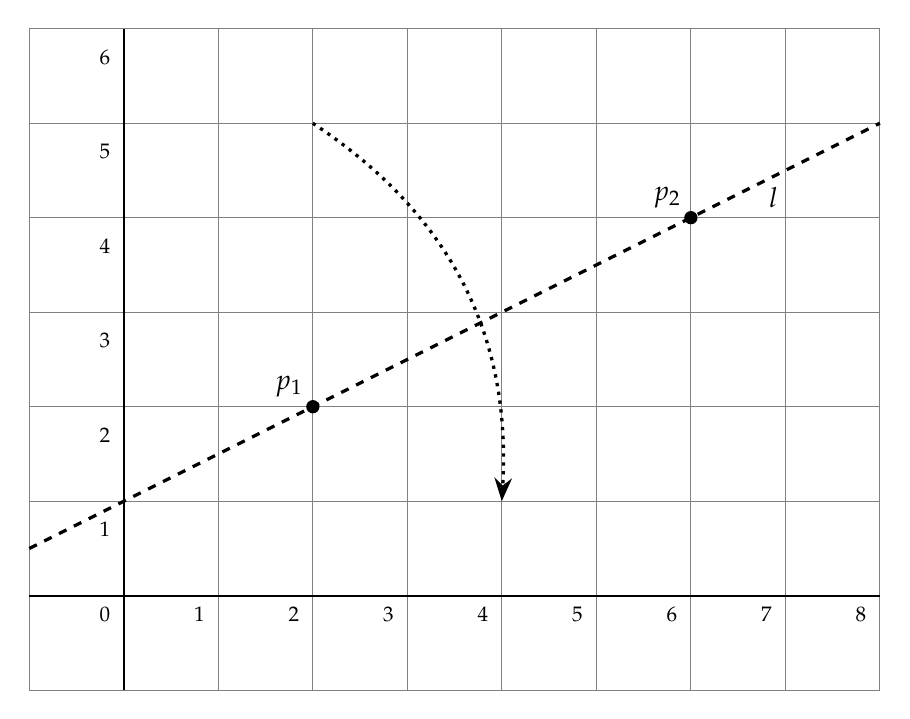
\begin{tikzpicture}[scale=1.2]
\draw[step=10mm,white!50!black,thin] (-1,-1) grid (8,6);
\draw[thick] (-1,0) -- (8,0);
\draw[thick] (0,-1) -- (0,6);
\foreach \x in {0,...,8}
  \node at (\x-.2,-.2) {\sm{\x}};
\foreach \y in {1,...,6}
  \node at (-.2,\y-.3) {\sm{\y}};
\coordinate (P1) at (2,2);
\coordinate (P2) at (6,4);
\draw[very thick,dashed] ($(P1)!-.75!(P2)$) -- node[very near end,below] {$l$} ($(P1)!1.5!(P2)$);
\fill (P1) circle(2pt) node[above left] {$p_1$};
\fill (P2) circle(2pt) node[above left] {$p_2$};

\draw[very thick,dotted,->,bend left=30] (2,5) to (4,1);
\end{tikzpicture}
\end{center}
%\end{figure}

\textbf{פיתוח משוואת הקיפול}

המשוואה של הקיפול 
$l$
מתקבלת מהקואורדינטות של 
$p_1$
ו-%
$p_2$:
השיפוע הוא המנה של הפרשי הקואורינטות ונקדות החיתוך עם ציר ה-%
$y$
מתקבלת מ-%
$p_1$:
\begin{equation}
\selectlanguage{english}
y - y_1 = \disfrac{y_2-y_1}{x_2-x_1}(x-x_1)\,.
\end{equation}

\vspace*{-3ex}
%\newpage

\textbf{דוגמה}

נסמן
$p_1=(2,2), p_2=(6,4)$. 
המשוואה של 
$l$  היא:
\begin{form}{2}
y-2&=&\disfrac{4-2}{6-2}(x-2)\\
y&=&\disfrac{1}{2}x+1\,.
\end{form}

%%%%%%%%%%%%%%%%%%%%%%%%%%%%%%%%%%%%%%%%%%%%%%%%%%%%%%%%%%%%%%%%
\newpage

\section{אקסיומה 2}\label{s.ax2}


\textbf{אקסיומה} 
נתונות שתי נקודות שונות
$p_1=(x_1,y_1)$, $p_2=(x_2,y_2)$,
קיים קיפול יחיד 
$l$
המניח את
$p_1$
על
$p_2$.

%\begin{figure}[H]
\begin{center}
\selectlanguage{english}
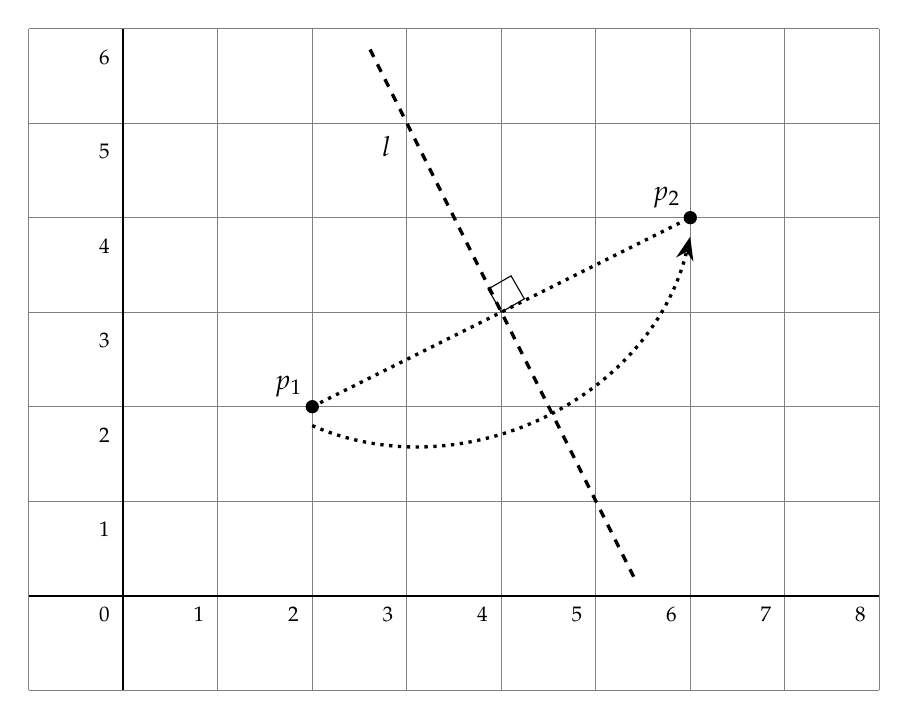
\begin{tikzpicture}[scale=1.2]
\draw[step=10mm,white!50!black,thin] (-1,-1) grid (8,6);
\draw[thick] (-1,0) -- (8,0);
\draw[thick] (0,-1) -- (0,6);
\foreach \x in {0,...,8}
  \node at (\x-.2,-.2) {\sm{\x}};
\foreach \y in {1,...,6}
  \node at (-.2,\y-.3) {\sm{\y}};
\coordinate (P1) at (2,2);
\coordinate (P2) at (6,4);
\coordinate (mid1) at ($(P1)!.5!(P2)$);
\coordinate (mid2) at ($(P1)!.5!(P2)+(-1,2)$);

\draw[rotate=30] (mid1) rectangle +(8pt,8pt);

\draw[very thick,dotted] (P1) -- (P2);
\draw[very thick,dashed] ($(mid1)!-1.4!(mid2)$) -- node[very near end,left,yshift=-12pt] {$l$} ($(mid1)!1.4!(mid2)$);
\fill (P1) circle(2pt) node[above left] {$p_1$};
\fill (P2) circle(2pt) node[above left] {$p_2$};

\draw[very thick,dotted,->,bend right=50] (2,1.8) to (6,3.8);
\end{tikzpicture}
\end{center}
%\end{figure}

\textbf{פיתוח משוואת הקיפול}

הקיפול 
$l$
הוא האנך האמצעי של
$\overline{p_1p_2}$.
השיפוע שלו הוא ההופכי השלילי של השיפוע של הקו המחבר את
$p_1$
ו-%
$p_2$.
$l$
עובר דרך נקודת האמצע בין שתי הנוקדות:
\begin{equation}
\selectlanguage{english}
y - \disfrac{y_1+y_2}{2} = -\disfrac{x_2-x_1}{y_2-y_1}\left(x-\disfrac{x_1+x_2}{2}\right)\,.\label{eq.midpoint1}
\end{equation}

\textbf{דוגמה}

נסמן
$p_1=(2,2), p_2=(6,4)$.
המשוואה של 
$l$
היא:
\begin{form}{2}
y-\left(\disfrac{2+4}{2}\right)&=&-\disfrac{6-2}{4-2}\left(x-\left(\disfrac{2+6}{2}\right)\right)\\
y&=&-2x+11\,.
\end{form}

%%%%%%%%%%%%%%%%%%%%%%%%%%%%%%%%%%%%%%%%%%%%%%%%%%%%%%%%%%%%%%%%
\newpage

\section{אקסיומה 3}\label{s.ax3}


\textbf{אקסיומה} 
נתונים שני קווים
$l_1$
ו-%
$l_2$,
קיים קיפול
$l$
המניח את
$l_1$ 
על
$l_2$.

%\begin{figure}[H]
\begin{center}
\selectlanguage{english}
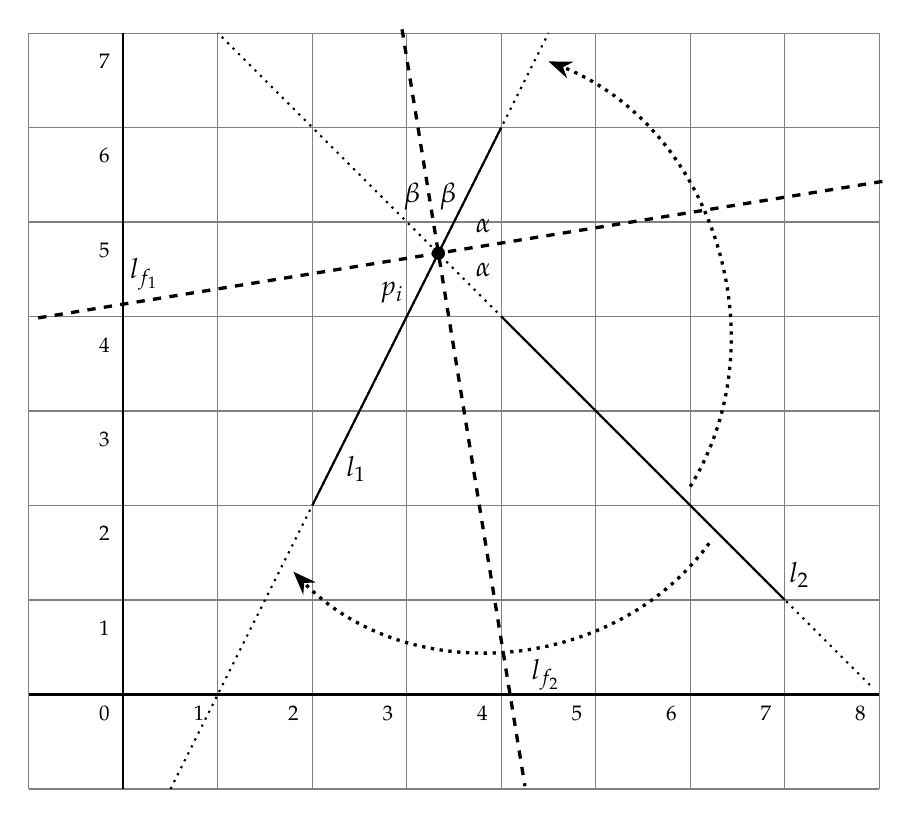
\begin{tikzpicture}[scale=1.2]
\draw[step=10mm,white!50!black,thin] (-1,-1) grid (8,7);
\draw[thick] (-1,0) -- (8,0);
\draw[thick] (0,-1) -- (0,7);
\foreach \x in {0,...,8}
  \node at (\x-.2,-.2) {\sm{\x}};
\foreach \y in {1,...,7}
  \node at (-.2,\y-.3) {\sm{\y}};
\coordinate (L1a) at (2,2);
\coordinate (L1b) at (4,6);
\draw[thick] (L1a) -- node[very near start,right,yshift=-4pt] {$l_1$} (L1b);
\draw[thick,dotted,name path=l1] ($(L1a)!-.75!(L1b)$) -- ($(L1a)!1.25!(L1b)$);
\coordinate (L2a) at (7,1);
\coordinate (L2b) at (4,4);
\draw[thick] (L2a) -- (L2b);
\draw[thick,dotted,name path=l2] ($(L2a)!-.3!(L2b)$) -- node[very near start,above,xshift=4pt,yshift=2pt] {$l_2$} ($(L2a)!2!(L2b)$);
\path [name intersections = {of = l1 and l2, by = {PM}}];
\fill (PM) circle(2pt) node[below left,xshift=-9pt,yshift=-7pt] {$p_i$};

\node[above right,xshift=10pt,yshift=4pt] at (PM) {$\alpha$};
\node[below right,xshift=10pt] at (PM) {$\alpha$};
\node[above left,xshift=-3pt,yshift=12pt] at (PM) {$\beta$};
\node[above right,xshift=-3pt,yshift=12pt] at (PM) {$\beta$};

\coordinate (B1a) at (0,4.13);
\coordinate (B1b) at (6,5.1);
\draw[very thick,dashed] ($(B1a)!-.15!(B1b)$) -- node[very near start,above] {$l_{f_1}$}  ($(B1a)!1.35!(B1b)$);

\coordinate (B2a) at (3,6.73);
\coordinate (B2b) at (4,.57);
\draw[very thick,dashed] ($(B2a)!-.05!(B2b)$) -- node[very near end,right,xshift=4pt,yshift=6pt] {$l_{f_2}$} ($(B2a)!1.25!(B2b)$);

\draw[very thick,dotted,->,bend right=50] (6,2.2) to (4.5,6.7);
\draw[very thick,dotted,->,bend left=50] (6.2,1.6) to (1.8,1.3);
\end{tikzpicture}
\end{center}
%\end{figure}

\textbf{פיתוח משוואת הקיפול עבור קווים מקבילים}

אם הקווים מקבילים, 
$l_1$
הוא
$y=mx+b_1$
ו-%
$l_2$
הוא
$y=mx+b_2$.
הקיפול הוא הקו המקביל ל-%
$l_1,l_2$ 
וחצי המרחק ביניהם:
$y=mx+\disfrac{b_1+b_2}{2}$.


\textbf{פיתוח משוואת הקיפול עבור קווים נחתכים}

אם הקווים נחתכים,
$l_1$ 
הוא
$y=m_1x+b_1$
ו-%
$l_2$
הוא
$y=m_2x+b_2$.


$p_i=(x_i,y_i)$,
נקודת החיתוך של שני הקווים, הוא:
\begin{form}{1.8}
m_1x_i+b_2&=&m_2x_i+b_2\\
x_i &=& \disfrac{b_2-b_1}{m_1-m_2}\\
y_i &=&m_1x_i+b_1\,.
\end{form}

\newpage

\textbf{דוגמה}

נסמן ב-%
$l_1$
את הקו
$y=2x-2$,
ונסמן ב-%
$l_2$
את הקו
$y=-x+8$.
נקודת החיתוך היא:
\begin{form}{2}
x_i&=&\disfrac{8-(-2)}{2-(-1)}=\disfrac{10}{3}\approx 3.33\\
y_i &=& 2\cdot\disfrac{10}{3}-2=\disfrac{14}{3}\approx 4.67\,.
\end{form}

\textbf{פיתוח משוואת השיפוע של חוצה הזווית}

שני קווים יוצרים זווית בנקודות החיתוך, למעשה, שני זוגות של זוויות קודקודיות. הקיפולים הם חוצי הזווית שלהן.

אם הזווית של
$l_1$
יחסית לציר ה-%
$x$
הוא
$\theta_1$ 
והזווית של 
$l_2$
יחסית לציר ה-%
$x$
הוא
$\theta_2$,
אזי קיפול הוא הקו היוצר זווית של
$\theta_b=\disfrac{\theta_1+\theta_2}{2}$
יחסית לציר ה-%
$x$.

$\tan\theta_1=m_1$
ו-%
$\tan\theta_2=m_2$
נתונים ו-%
$m_b$,
השיפוע של חוצה הזווית, הוא:
\[
m_b=\tan\theta_b=\tan\disfrac{\theta_1+\theta_2}{2}\,.
\]
פיתוח המשוואה מחייב שימוש בשוויונות הטריגונומטריות:%
\footnote{%
פיתוח המשוואות הללו נתון בנספח%
~\ref{a.tangent}.}
\begin{form}{2.2}
\tan(\alpha_1+\alpha_2)&=& \disfrac{\tan\alpha_1+\tan\alpha_2}{1-\tan\alpha_1\tan\alpha_2}\\
\tan \disfrac{\alpha}{2}&=& \disfrac{-1\pm\sqrt{1+\tan^2\alpha}}{\tan \alpha}\,.
\end{form}
תחילה נמצא את
$m_s$,
השיפוע של
$\theta_1+\theta_2$:
\[
m_s=\tan(\theta_1+\theta_2)= \disfrac{m_1+m_2}{1-m_1m_2}\,.
\]
אחר כך נמצא את 
$m_b$,
השיפוע של חוצה הזווית:
\begin{form}{2.1}
m_b&=& \tan\disfrac{\theta_1+\theta_2}{2}\\
&=&\disfrac{-1\pm\sqrt{1+\tan^2(\theta_1+\theta_2)}}{\tan (\theta_1+\theta_2)}\\
&=&\disfrac{-1\pm\sqrt{1+m_s^2}}{m_s}\,.
\end{form}

\newpage

\textbf{דוגמה}

עבור הקווים
$y=2x-2$
ו-%
$y=-x+8$,
השיפוע של חוצה הזווית הוא:
\begin{form}{2.1}
m_s=\disfrac{2+(-1)}{1-(2 \cdot -1)}=\disfrac{1}{3}\\
m_b=\disfrac{-1\pm\sqrt{1+(1/3)^2}}{1/3}=-3\pm \sqrt{10}\approx -6.16,\; 0.162\,.
\end{form}

\textbf{פיתוח משוואת הקיפול}

נפתח את המשוואה של הקיפול
$l_{f_1}$
באיור עם שיפוע חיובי. אנו יודעים את הקואורדינטות של נקודת החיתוך של שני הקווים
$m_i=\left(\disfrac{10}{3},\disfrac{14}{3}\right)$:
\begin{form}{2}
\disfrac{14}{3} &=& (-3+\sqrt{10}) \cdot \disfrac{10}{3} + b\\ b&=&\disfrac{44-10\sqrt{10}}{3}\\
y&=& (-3+\sqrt{10})x + \disfrac{44-10\sqrt{10}}{3}\approx 0.162x+4.13\,.
\end{form}


%%%%%%%%%%%%%%%%%%%%%%%%%%%%%%%%%%%%%%%%%%%%%%%%%%%%%%%%%%%%%%%%
\newpage

\section{אקסיומה 4}\label{s.ax4}


\textbf{אקסיומה} 
נתונים נקודה
$p_1$
וקו
$l_1$,
קיים קיפול יחיד
$l$
הניצב ל-%
$l_1$
שעובר דרך
$p_1$.
%\begin{figure}[H]
\begin{center}
\selectlanguage{english}
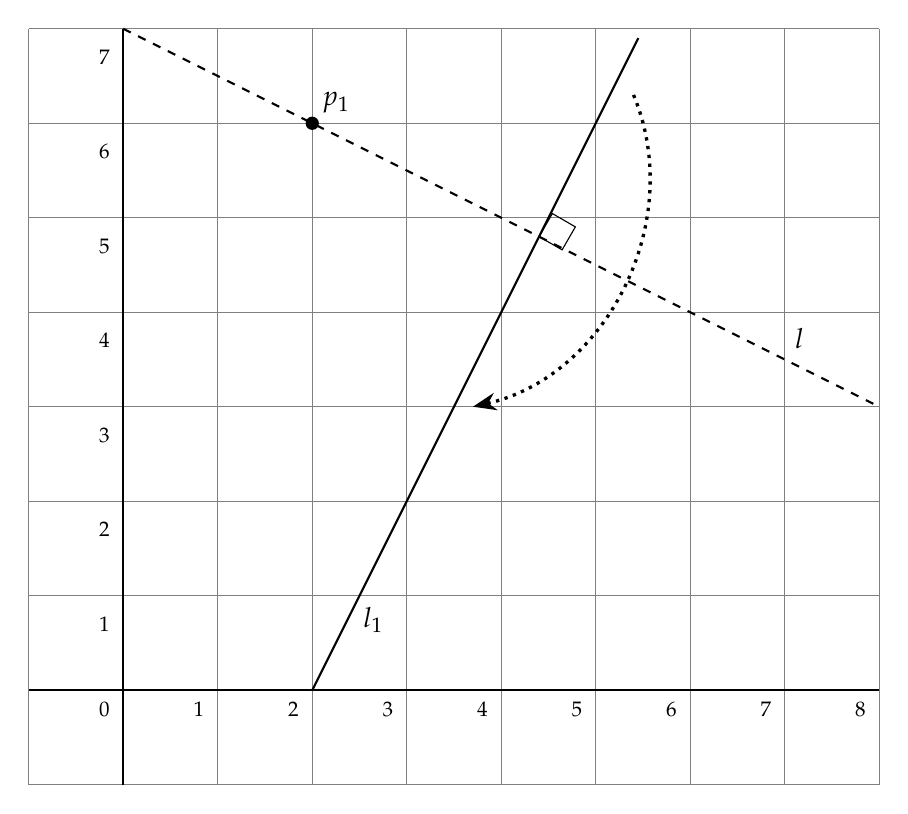
\begin{tikzpicture}[scale=1.2]
\draw[step=10mm,white!50!black,thin] (-1,-1) grid (8,7);
\draw[thick] (-1,0) -- (8,0);
\draw[thick] (0,-1) -- (0,7);
\foreach \x in {0,...,8}
  \node at (\x-.2,-.2) {\sm{\x}};
\foreach \y in {1,...,7}
  \node at (-.2,\y-.3) {\sm{\y}};
\coordinate (L1a) at (2,0);
\coordinate (L1b) at (5,6);
\draw[thick] (L1a) -- node[very near start,right,yshift=-4pt] {$l_1$} ($(L1a)!1.15!(L1b)$);
\fill (2,6) circle (2pt) node[above right] {$p_1$};
\draw[thick,dashed] (0,7) -- node[very near end,above right] {$l$} (8,3);
\coordinate (intersection) at (4.4,4.8);
\draw[rotate=-30] (intersection) rectangle +(8pt,8pt);

\draw[very thick,dotted,->,bend left=50] (5.4,6.3) to (3.7,3);
\end{tikzpicture}
\end{center}
%\end{figure}

\textbf{פיתוח משוואת הקיפול}

נסמן את
$y = m_1x + b_1$
ב-%
$l_1$,
ונסמן
$p_1=(x_1,y_1)$. 
$l$
ניצב ל-%
$l_1$
לכן השיפוע שלו הוא
$-\disfrac{1}{m_1}$.
הקו עובר דרך
$p_1$
ונוכל לחשב את החיתוך שלו 
$b$
ולכתוב את המשוואה:
\begin{form}{2}
y_1=-\disfrac{1}{m} x_1 + b\\
b= \disfrac{(my_1+x_1)}{m}\\
y=-\disfrac{1}{m} x +\disfrac{(my_1+x_1)}{m}\,.
\end{form}
\textbf{דוגמה}

נסמן ב-%
$p_1$
את הנקודה
$(2,6)$
ונסמן ב-%
$l_1$
את הקו
$y=2x-4$.
המשוואה של הקיפול
$l$
היא:
\[
y=-\disfrac{1}{2}x + \disfrac{2\cdot 6 + 2}{2}=-\disfrac{1}{2}x + 7\,.
\]


%%%%%%%%%%%%%%%%%%%%%%%%%%%%%%%%%%%%%%%%%%%%%%%%%%%%%%%%%%%%%%%%
\newpage

\section{אקסיומה 5}\label{s.ax5}


\textbf{אקסיומה} 
נתונות נקודות
$p_1,p_2$
ונתון קן
$l_1$,
קיים קיפול
$l$
המניח את
$p_1$
מעל
$l_1$
והעובר דרך
$p_2$.

%\begin{figure}[H]
\begin{center}
\selectlanguage{english}
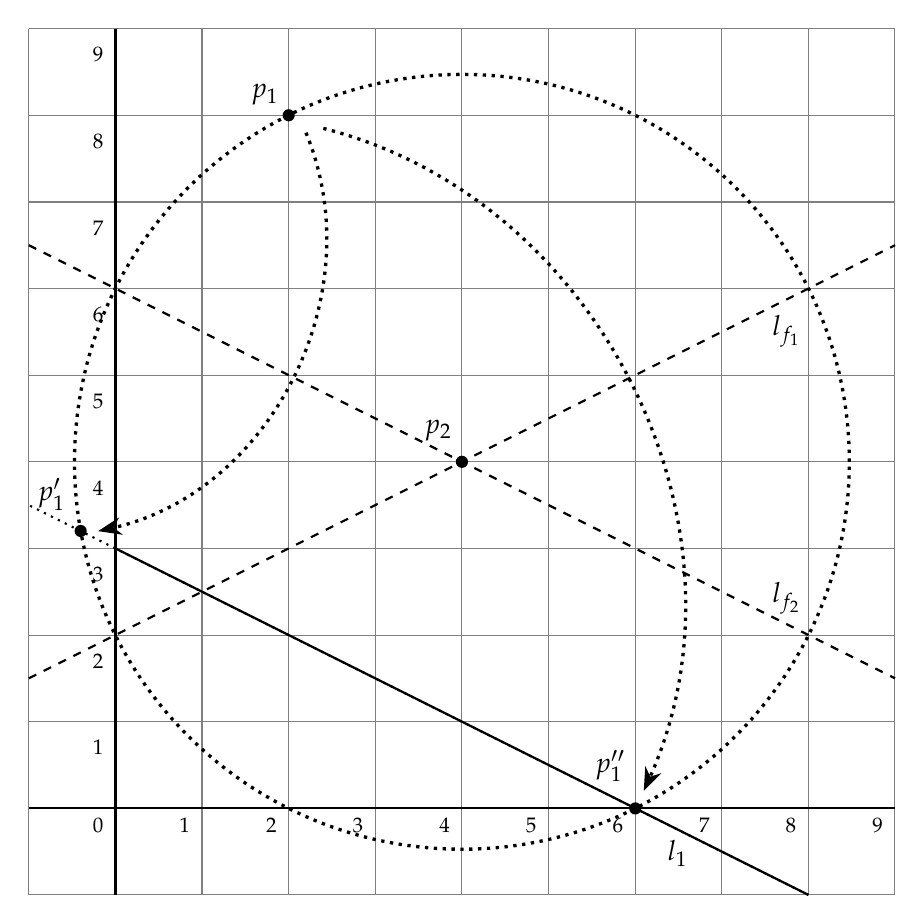
\begin{tikzpicture}[scale=1.1]
\draw[step=10mm,white!50!black,thin] (-1,-1) grid (9,9);
\draw[thick] (-1,0) -- (9,0);
\draw[thick] (0,-1) -- (0,9);
\foreach \x in {0,...,9}
  \node at (\x-.2,-.2) {\sm{\x}};
\foreach \y in {1,...,9}
  \node at (-.2,\y-.3) {\sm{\y}};
\coordinate (L1a) at (0,3);
\coordinate (L1b) at (8,-1);
\draw[thick] (L1a) -- node[near end,below right,xshift=8pt,yshift=-8pt] {$l_1$} (L1b);
\coordinate (P1) at (2,8);
\fill (P1) circle (2pt) node[above left] {$p_1$};
\coordinate (P2) at (4,4);
\fill (P2) circle (2pt) node[above left,yshift=4pt] {$p_2$};
\draw[thick,dotted,name path=L1] (8,-1) -- (-1,3.5);
\node[very thick,dotted,draw, name path = circle] at (P2)
    [circle through = (P1)] {};

\path [name intersections = {of = circle and L1, by = {P1P,P1PP}}];
\fill (P1P) circle (2pt) node[above left,xshift=-2pt,yshift=4pt] {$p_1'$};
\fill (P1PP) circle (2pt) node[above left,yshift=6pt] {$p_1''$};

\coordinate (f1) at (0,6);
\draw[thick,dashed] ($(f1)!-.25!(P2)$) -- node[very near end,above] {$l_{f_2}$} ($(f1)!2.25!(P2)$);
\coordinate (f2) at (0,2);
\draw[thick,dashed] ($(f2)!-.25!(P2)$) -- node[very near end,below,yshift=-2pt] {$l_{f_1}$} ($(f2)!2.25!(P2)$);

\draw[very thick,dotted,->,bend left=50] (2.2,7.8) to (-.2,3.2);
\draw[very thick,dotted,->,bend left=50] (2.4,7.85) to (6.1,.2);
\end{tikzpicture}
\end{center}
%\end{figure}

עבור זוג נקודות נתון וקו נתון, יכולים להיות אפס, אחד או שני קיפולים.

\textbf{פיתוח משוואות עבור השיקופים}

נסמן ב-%
$l$
את הקיפול העובר דרך
$p_2$,
ונסמן ב-%
$p_1'$
את השיקוף של
$p_1$
מסביב ל-%
$l$.
האורך של
$\overline{p_1p_2}$
שווה לאורך של
$\overline{p_2p_1}'$.
המקום הגיאומטרי של נקודות הנמצאות במרחק
$\overline{p_1p_2}$
\textbf{מ-}%
$p_2$
הוא המעגל שמרכזו
$p_2$
והרדיוס שלו הוא האורך
$\overline{p_1p_2}$. 
נקודות החיתוך של מעגל זה עם הקו
$l_1$
הן המקומות האפשריים עבור
$p_1'$.

נסמן
$y=m_1x + b_1$
ב-%
$l_1$,
ונסמן
$p_1=(x_1,y_1)$, $p_2=(x_2,y_2)$.
המשוואה של המעגל שמרכזו
$p_2$
עם רדיוס באורך של
$\overline{p_1p_2}$
היא:
\begin{form}{1.5}
(x-x_2)^2 + (y-y_2)^2 = r^2\\
r^2= (x_2-x_1)^2 + (y_2-y_1)^2\quad \textrm{\R{כאשר}}\,.
\end{form}
נציב את המשוואה של הקו לתוך המשוואה של המעגל:
\[
(x-x_2)^2+((m_1x+b_1)-y_2)^2=(x-x_2)^2+(m_1x+(b_1-y_2))^2=r^2\,,
\]
ונקבל משוואה ריבועית עבור קואורדינטות ה-%
$x$
של נקודות החיתוך האפשריות:
\begin{equation}
\selectlanguage{english}
x^2(1+m_1^2) \,+\, 2(-x_2+m_1b-m_1y_2)x \,+\, (x_2^2 + (b_1^2 - 2b_1y_2+y_2^2)-r^2)=0\,.\label{eq.intersections}
\end{equation}
למשוואה ריבועית יש לכל היותר שני פתרונות
$x_1',x_1''$,
ונחשב את 
$y_1',y_1''$
מ-%
$y=m_1x+b_1$.
נקודות השיקוף הן
$p_1'=(x_1',y_1'), p_1''=(x_1'',y_1'')$.

\textbf{דוגמה}

נסמן ב-%
$p_1$
את הנקודה
$(2,8)$
ונסמן ב-%
$p_2$
את הנקודה
$(4,4)$.
נסמן ב-%
$l_1$ 
את הקו
$y=-\disfrac{1}{2}x +3$.
משוואת המעגל היא:
\[
(x-4)^2 + (y-4)^2 = r^2=(4-2)^2+(4-8)^2=20\,.
\]
נציב את המשוואה של הקו לתוך המשוואה של המעגל ונפשט כדי לקבל משוואה ריבועית עבור קואורדינטות ה-%
$x$
של נקודות החיתוך )אפשר גם להשתמ משוואה%
~\L{\ref{eq.intersections}}(:
\begin{form}{1.5}
(x-4)^2 + \left(\left(-\disfrac{1}{2}x+3\right)-4\right)^2&=&20\\
\disfrac{5}{4}x^2-7x-3 &=&0\\
5x^2 -28x -12&=&0\\
(5x+2)(x-6)&=&0\,.
\end{form}
שתי נקודות חיתוך הן:
\[
p_1'=\left(-\disfrac{2}{5},\disfrac{16}{5}\right) = (-0.4,3.2)\,,\quad p_1''=(6,0)\,.
\]

\textbf{פיתוח המשוואות של הקיפולים}

הקיפולים יהיו האנכים האמצעיים של
$\overline{p_1p_1'}$
ו-%
$\overline{p_1p_1''}$.
המשוואה של אנך אמצעי נתונה על ידי משוואה%
~\L{\ref{eq.midpoint1}},
שנעתיק כאן עבור
$p_1'$:
\begin{equation}
\selectlanguage{english}
y - \disfrac{y_1+y_1'}{2} = -\disfrac{x_1'-x_1}{y_1'-y_1}\left(x-\disfrac{x_1+x_1'}{2}\right)\,.\label{eq.midpoint2}
\end{equation}

\newpage

\textbf{דוגמה}

עבור
$p_1=(2,8)$
ו-%
$p_1'=\left(-\disfrac{2}{5},\disfrac{16}{5}\right)$,
משוואת הקיפול עבור
$l_{f_1}$
היא:
\begin{form}{2}
y-\disfrac{8+(16/5)}{2}&=&-\disfrac{(-2/5)-2}{(16/5)-8}\left(x-\disfrac{2+\left(-2/5\right)}{2}\right)\\
y&=&-\disfrac{1}{2}x+6\,.
\end{form}

עבור
$p_1=(2,8)$
ו-%
$p_1''=(6,0)$,
משוואת הקיפול עבור
$l_{f_2}$ 
היא:
\begin{form}{2}
y-\disfrac{8+0}{2}&=&-\disfrac{6-2}{0-8}\left(x-\disfrac{2+6}{2}\right)\\
y&=&\disfrac{1}{2}x+2\,.
\end{form}

%%%%%%%%%%%%%%%%%%%%%%%%%%%%%%%%%%%%%%%%%%%%%%%%%%%%%%%%%%%%%%%%

\newpage

\section{אקסיומה 6}\label{s.ax6}

\textbf{אקסיומה}                          
נתונות שתי נקודות
$p_1$
ו-%
$p_2$
ונתונים שני קווים
$l_1$
ו-%
$l_2$,
קיים קיפול
$l$
המניח את 
$p_1$
על ל-%
$l_1$
ו-%
$p_2$
על ל-%
$l_2$.

%\begin{figure}[H]
\begin{center}
\selectlanguage{english}
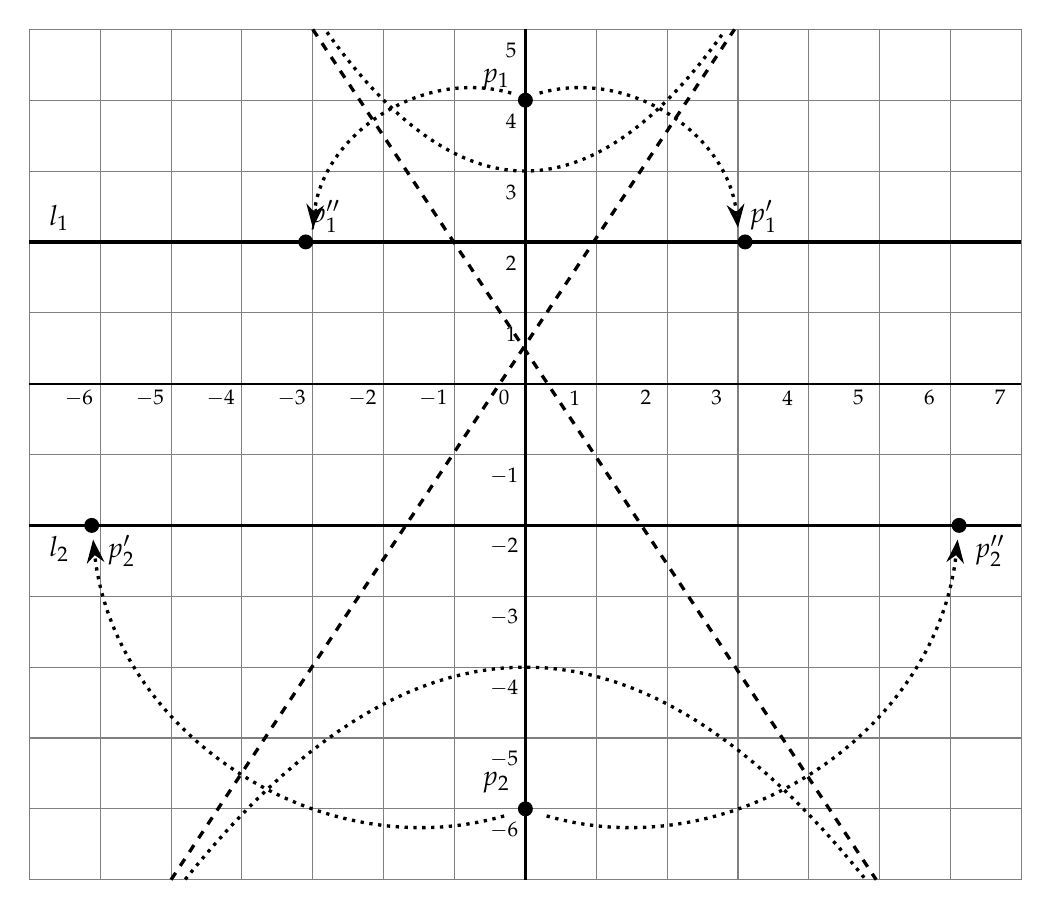
\begin{tikzpicture}[scale=.9]
\draw[step=10mm,white!50!black,thin] (-7,-7) grid (7,5);
\draw[thick] (-7,0) -- (7,0);
\draw[thick] (0,-7) -- (0,5);
\foreach \x in {-6,...,7}
  \node at (\x-.3,-.2) {\sm{\x}};
\foreach \y in {1,...,5}
  \node at (-.2,\y-.3) {\sm{\y}};
\foreach \y in {-6,...,-1}
  \node at (-.3,\y-.3) {\sm{\y}};
  
\coordinate (P1) at (0,4);
\fill (P1) circle (3pt) node[above left,xshift=-2pt] {$p_1$};
\coordinate (P2) at (0,-6);
\fill (P2) circle (3pt) node[above left,xshift=-2pt,yshift=2pt] {$p_2$};

\coordinate (P1P) at (3.1,2);
\fill (P1P) circle (3pt) node[above right,xshift=-2pt] {$p_1'$};
\coordinate (P2P) at (-6.12,-2);
\fill (P2P) circle (3pt) node[below right,xshift=2pt] {$p_2'$};

\coordinate (P1PP) at (-3.1,2);
\fill (P1PP) circle (3pt) node[above right,xshift=-2pt] {$p_1''$};
\coordinate (P2PP) at (6.12,-2);
\fill (P2PP) circle (3pt) node[below right,xshift=2pt] {$p_2''$};

\draw[very thick] (-7,2) -- node[very near start,above,xshift=-34pt] {$l_1$} (7,2);
\draw[very thick] (-7,-2) -- node[very near start,below,xshift=-34pt] {$l_2$} (7,-2);

\draw[domain=-4.8:4.8,samples=50,very thick,dotted] plot (\x,{-.13*\x*\x-4});
\draw[domain=-2.8:2.8,samples=50,very thick,dotted] plot (\x,{.25*\x*\x+3});

\draw[very thick,dashed] (-5,-7) -- (2.95,5);
\draw[very thick,dashed] (-3,5) -- (4.95,-7);

\draw[very thick,dotted,->,bend left=50] (.2,4.1) to (3,2.2);
\draw[very thick,dotted,->,bend left=50] (-.3,-6.1) to (-6.1,-2.2);

\draw[very thick,dotted,->,bend right=50] (-.2,4.1) to (-3,2.2);
\draw[very thick,dotted,->,bend right=50] (.3,-6.1) to (6.1,-2.2);
\end{tikzpicture}
\end{center}
%\end{figure}

עבור זוג נקודות נתון וזוג קווים נתון, יכולים להיות אפס, אחד, שניים או שלושה קיפולים. ניתן למצוא הוכחה ב-%
\cite[פרק $10$]{martin};
בנספח 
\ref{a.number-of-tangents}
הבאנו דוגמאות גרפיות לארבעת האפשרויות.

קיפול המניח את 
$p_i$
על
$l_i$
הוא קו שמרחקו ל-%
$p_i$
שווה למרחקו ל-%
$l_i$.
המקום הגיאומטרי של נקודות שהן במרחק שווה מנקודה
$p_i$
ומקו
$l_i$
הוא פרבולה עם מוקד 
\L{(focus)}
$p_i$
ומדריך
\L{(directrix)}
$l_i$.
קיפול הוא כל קו המשיק לפרבולה. הצדקה מפורטת של טיעון זה נמצא בנספח%
~\ref{a.parabola}.

כדי שהקיפול יניח בו-זמנית את 
$p_1$
על ל-%
$l_1$
ו-%
$p_2$
על ל-%
$l_2$,
הוא חייב להיות משיק משותף לשתי הפרבולות.

המשוואה עבור פרבולה שרירותית די מסובכת, לכן נגביל את הדיון לפרבולה שציר ה-%
$y$
הוא ציר הסמטריה. אין כאן מגבלה משמעותית כי עבור כל פרבולה קיימים הזזה וסיבוב המעבירים אותה כך שציר הסמטריה שלה הוא ציר ה-%
$y$.

נביא גם דוגמה עם פרבולה שציר הסמטריה שלה הוא ציר ה-%
$x$.

\newpage

\textbf{פיתוח הנקודה של הקיפול}

תהי
$(0,f)$
מוקד של פרבולה עם מדריך
$y=d$.
נגדיר
$p=f-d$,
האורך )עם הסימן( של קטע הקו בין המוקד למדריך.%
\footnote{%
השתמשנו בסימון
$p_i$
עבור נקודות, כך שהשימוש כאן ב-%
$p$
עלול לבלבל, אבל סימון זה מקובל. השם הפורמלי עבור
$p$
הוא מחצית ה-%
\L{latus rectum}.}
אם קודקוד 
\L{(vertex)}
הפרבולה נמצא על ציר ה-%
$x$,
המשוואה של הפרבולה היא
$y=\disfrac{x^2}{2p}$.
כדי להזיז את הפרבולה למעלה או למטה על ציר ה-%
$y$,
כך שהקודקוד שלה היא
$(0,h)$,
יש להוסיף 
$h$
למשוואת הפרבולה:
$y=\disfrac{x^2}{2p}+h$.
\begin{center}
\selectlanguage{english}
\begin{tikzpicture}[scale=1]
\draw (-6,0) -- node[very near start,below,xshift=-32pt] {$x$-\textsf{axis}}(6,0);
\draw (0,-3) -- node[very near start,right,yshift=-20pt] {$y$-\textsf{axis}}(0,4.5);
\draw[very thick] (-6,-2) -- node[near start,below] {\textsf{directrix} $\quad y=-2$} (6,-2);
\draw[domain=-5:5,samples=50,very thick,dotted] plot (\x,{\x*\x/8+1});
\coordinate (F) at (0,4);
\fill (F) circle (2pt) node[left,xshift=-2pt,yshift=0pt] {$(0,f)=(0,4)$} node[above left,xshift=-2pt,yshift=4pt] {\textsf{focus}};
\fill (0,-2) circle (2pt);
\fill (0,1) circle (2pt) node[below left] {\textsf{vertex}} node[below left,yshift=-10pt] {$(0,1)$};
\draw[<->] (2,-1.9) -- node[fill=white] {$p=6$} +(0,5.8);
\draw[<->] (1,.1) -- node[fill=white] {$h=1$} +(0,.8);
\end{tikzpicture}
\end{center}
נגדיר
$a=2ph$
כך שמשוואת הפרבולה היא:
\begin{form}{1.5}
y=\disfrac{x^2}{2p}+\disfrac{a}{2p}\\
x^2-2py+a=0\,.
\end{form}
עבור הפרבולה באיור למעלה המשוואה היא:
\begin{form}{1}
x^2-2\cdot 6\,y + 2\cdot 6 \cdot 1=0\\
x^2-12y +12=0\,.
\end{form}
נציב את המשוואה של קו 
\textbf{שרירותי}
$y=mx+b$
במשוואה עבור הפרבולה ונקבל משוואה עבור נקודות החיתוך של הקו והפרבולה:
\begin{form}{1.5}
x^2-2p(mx+b)+a=0\\
x^2+(-2mp)x+(-2pb+a)=0\,.
\end{form}
הקו יהיה משיק לפרבולה אם ורק אם למשוואה ריבועית זו קיים 
\textbf{בדיוק}
פתרון אחד אם ורק אם הדיסקרימננטה היא אפס:
\[
(-2mp)^2\:-\:4\cdot 1\cdot (-2pb+a)=0\,.
\]
לאחר פישוט מתקבלת:
\begin{equation}
\selectlanguage{english}
m^2p^2+2pb-a=0\,.\label{eq.disc}
\end{equation}
משוואה זו עם המשתנה 
$m$ 
היא המשוואה עבור השיפועים של המשיקים לפרבולה. קיימים אינסוף משיקים כי עבור כל 
$m$,
קיים
$b$
שגורם למשיק לזוז למעלה או למטה.%
\footnote{%
פרט כמובן עבור קו המקביל לציר הסמטריה.%
}

כדי למצוא את המשיקים המשותפים לשתי הפרבולות, יש לפתור את המשוואות של שתי הפרבולות, משוואות עם שני משתנים
$m$
ן-%
$b$.

%%%%%%%%%%%%%%%%%%%%%%%%%%%%%%%%%%%%%%%%%%%%%%%%%%%%%%%%%%%%%%%%


\textbf{דוגמה}

פרבולה 1: מוקד
$(0,4)$,
מדריך
$y=2$,
קודקוד,
$(0,3)$
ו-%
$p=2$, $a=2\cdot 2\cdot 3=12$.
משוואת הפרבולה היא:
\[
\begin{array}{l}
x^2-2\cdot 2y +12=0\,.
\end{array}
\]
נציב לתוך משוואה%
~\L{\ref{eq.disc}}
ונפשט:
\[
m^2+b-3=0\,.
\]
פרבולה 2: מוקד
$(0,-4)$,
מדריך
$y=-2$,
קודקוד,
$(0,-3)$
ו-%
$p=-2$, $a=2\cdot -2\cdot -3=12$.
משוואת הפרבולה היא:
\[
x^2-2\cdot (-2)y+12=0\,.
\]
נציב לתוך משווארה%
~\L{\ref{eq.disc}}
ופשט:
\[
m^2-b-3=0\,.
\]
הפתרונות של שתי המשוואות:
\begin{form}{1.5}
m^2+b-3=0\\
m^2-b-3=0\,,
\end{form}
הם
$m=\pm\sqrt{3}\approx \pm 1.73$
ן-%
$b=0$.
המשיקים המשותפים שהם הקיפולים הם:
\[
y=\sqrt{3}x\,,\quad y=-\sqrt{3}x\,.
\]

%%%%%%%%%%%%%%%%%%%%%%%%%%%%%%%%%%%%%%%%%%%%%%%%%%%%%%%%%%%%%%%%

\textbf{דוגמה}

פרבולה 1 ללא שינוי.

פרבולה 2: מוקד
$(0,-6)$,
מדריך
$y=-2$,
קודקוד,
$(0,-4)$
ו-%
$p=-4$, $a=2\cdot -4\cdot -4=32$.
משוואת הפרבולה היא:
\[
x^2-2\cdot (-4)y +32=0\,.
\]
נציב לתוך משווארה%
~\L{\ref{eq.disc}}
ונפשט:
\[
2m^2-b-4=0\,.
\]
הפתרונות של שתי המשוואות:
\begin{form}{1.5}
m^2+b-3=0\\
2m^2-b-4=0\,,
\end{form}
הם
$m=\pm\sqrt{\disfrac{7}{3}}\approx \pm 1.53$
ו-%
$b=\disfrac{2}{3}$.
יש שני משיקים משותפים שהם קיפולים:
\[
y=\sqrt{\disfrac{7}{3}}x+\disfrac{2}{3}\,,\quad y=-\sqrt{\disfrac{7}{3}}x+\disfrac{2}{3}\,.
\]

%%%%%%%%%%%%%%%%%%%%%%%%%%%%%%%%%%%%%%%%%%%%%%%%%%%%%%%%%%%%%%%%

\textbf{דוגמה}

כעת נגדיר פרבולה שציר הסמטריה שלה הוא ציר ה-%
$x$.

פרבולה 1 ללא שינוי.

פרבולה 2: מוקד
$(4,0)$,
מדריך
$x=2$,
קודקוד,
$(3,0)$
ו-%
$p=2$, $a=2\cdot 2\cdot 3=12$.
משוואת הפרבולה היא:
\[
y^2-4x+12 = 0\,.
\]
שימו לב שזו משוואה עם 
$x$
ו-%
$y^2$
במקום
$x^2$
ו-%
$y$,
כך שלא ניתן להשתמש במשוואה%
~\L{\ref{eq.disc}}
ונצטרך לפתח את משוואות מחדש.

נציב את המשוואה עבור קו:
\begin{form}{1.5}
(mx+b)^2-4x+12=0\\
m^2x^2+(2mb-4)x+(b^2+12)=0\,,
\end{form}
נשווה את הדיסקרימננטה לאפס ונפשט:
\begin{form}{1.5}
(2mb-4)^2\:-\:4m^2(b^2+12)=0\\
-3m^2-mb+1=0\,.
\end{form}
אם ננסה לפתור את שתי המשוואות:
\begin{form}{1.5}
m^2+b-3=0\\
-3m^2-mb+1=0\,,
\end{form}
נקבל 
משוואה ממעלה שלוש במשתנה
$m$:
\begin{equation}
\selectlanguage{english}
m^3-3m^2-3m+1=0\,.\label{eq.cubic}
\end{equation}
למשוואה ממעלה שלוש יש לפחות פתרון ממשי אחד ולכן היותר שלושה פתרונות ממשיים, לכן יכול להיות אחד, שניים או שלשה משיקים משתופים. אפשר שלא יהיה אף משיק אחד אם אין פתרון לשתי המשוואות, למשל, כאשר פרבולה אחת נמצאת בתוך השנייה: 
$y=x^2$, $y=x^2+1$.

המשוואה למציאת פתרונות למשוואה ממעלה שלוש די מסובכת, לכן השתמשתי במחשבון באינטרנט וקיבלתי שלושה פתרונות:
\[
m=3.73\,, \;m=-1\,, \; m=0.27\,.
\]
אם נבחר
$m=0.27$, $b=3-m^2=2.93$,
משוואת הקיפול היא:
\[
y=0.27x+2.93\,.
\]
מהצורה של המשוואה%
~\L{\ref{eq.cubic}},
נוכל לנחש ש-%
$1$
או
$-1$
הוא פתרון:
\begin{form}{1.4}
1^3-3\cdot 1^2-3\cdot 1+1=-4\\
(-1)^3-3\cdot (-1)^2-3\cdot(-1)+1=0\,.
\end{form}
נחלק את המשוואה%
~\L{\ref{eq.cubic}}
ב-%
$m-(-1)=m+1$
ונקבל משוואה ריבועית
$m^2-4m+1$
ששורשיה הם
$2\pm\sqrt{3}\approx 3.73, 0.27$.


%%%%%%%%%%%%%%%%%%%%%%%%%%%%%%%%%%%%%%%%%%%%%%%%%%%%%%%%%%%%%%%%

\textbf{פיתוח המשוואות של השיקופים}

נפתח את המיקום של 
$p_1'=(x_1',y_1')$,
השיקוף של
$p_1=(x_1,y_1)$
מסביב למשיק
$l_t$
שהמשוואה שלה היא
$y=m_tx+b_t$.
הפיתוח זהה עבור כל משיק ועבור 
$p_2$.

כדי לשקף את
$p_1$
מסביב ל-%
$l_t$,
נמצא את הקו
$l_p$
עם המשוואה
$y=m_px+b_p$
שניצב ל-%
$l_t$
ועובר דרך
$p_1$:
\begin{form}{2}
y=-\disfrac{1}{m_t}x+b_p\\
y_1=-\disfrac{1}{m_t}x_1+b_p\\
y=\disfrac{-x}{m_t}+\left(y_1+\disfrac{x_1}{m_t}\right)\,.
\end{form}
אז נמצא את נקודת החיתוך 
$p_t=(x_t,y_t)$
של
$l_t$
ו-%
$l_p$:
\begin{form}{3}
m_tx_t+b_t=\disfrac{-x_t}{m_t}+\left(y_1+\disfrac{x_1}{m_t}\right)\\
x_t=\disfrac{\left(y_1+\disfrac{x_1}{m_t}-b_t\right)}{\left(m_t+\disfrac{1}{m_t}\right)}\\
y_t=m_tx_t+b_t\,.
\end{form}
קל למצוא את השיקוף
$p_1'$
כי נקודת החיתוך
$p_t$
היא נקודת האמצע בין
$p_1$
והשיקוף שלו
$p_1'$:
\begin{form}{2}
x_t=\disfrac{x_1+x_1'}{2}\,,\quad y_t=\disfrac{y_1+y_1'}{2}\\
x_1'=2x_t-x_1\,,\quad y_1'=2y_t-y_1\,.
\end{form}

\newpage

\textbf{דוגמה}

נסמן
$p_1=(0,4)$
ונסמן ב-%
$l_1$
את
$y=\sqrt{3}x$:
\begin{form}{2.2}
x_t=\disfrac{\left(4+\disfrac{0}{\sqrt{3}}-0\right)}{\left(\sqrt{3}+\disfrac{1}{\sqrt{3}}\right)}=\sqrt{3}\\
y_t=\sqrt{3}\sqrt{3}+0=3\\
x_1'=2x_t-x_1=2\sqrt{3}-0=2\sqrt{3}\approx 3.46\\
y_1'=2y_t-y_1=2\cdot 3 - 4 = 2\,.
\end{form}

%%%%%%%%%%%%%%%%%%%%%%%%%%%%%%%%%%%%%%%%%%%%%%%%%%%%%%%%%%%%%%%%
\newpage

\section{אקסיומה 7}\label{s.ax7}

\textbf{אקסיומה} 
נתונה נקודה אחת
$p_1$,
ונתונים שני קווים
$l_1$,
$l_2$,
קיים קיפול
$l$
הניצב ל-%
$l_2$
שהמניח את
$p_1$
על ל-%
$l_1$.

%\begin{figure}[H]
\begin{center}
\selectlanguage{english}
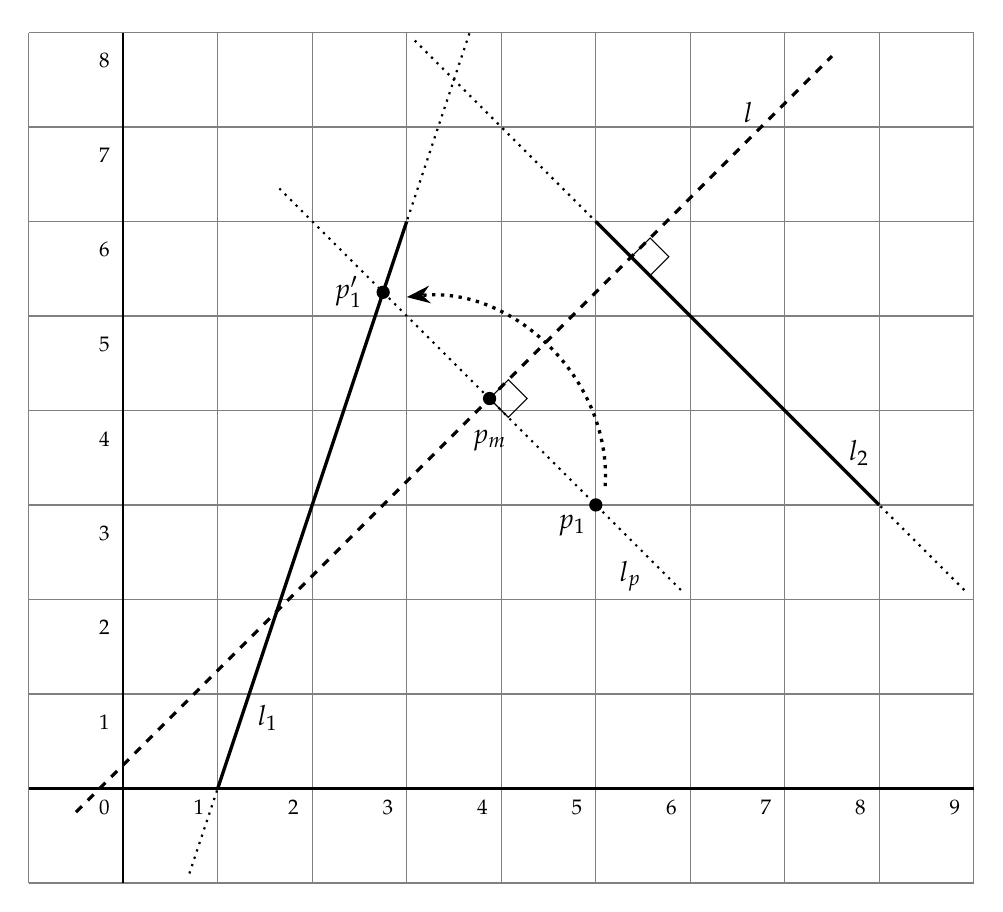
\begin{tikzpicture}[scale=1.2]
\draw[step=10mm,white!50!black,thin] (-1,-1) grid (9,8);
\draw[thick] (-1,0) -- (9,0);
\draw[thick] (0,-1) -- (0,8);
\foreach \x in {0,...,9}
  \node at (\x-.2,-.2) {\sm{\x}};
\foreach \y in {1,...,8}
  \node at (-.2,\y-.3) {\sm{\y}};
  
\coordinate (P1) at (5,3);
\fill (P1) circle (2pt) node[below left] {$p_1$};

\coordinate (P1P) at (2.75,5.25);
\fill (P1P) circle (2pt) node[left,xshift=-4pt] {$p_1'$};

\draw[very thick] (1,0) -- node[very near start,right,xshift=2pt] {$l_1$} (3,6);
\draw[very thick,name path=l2] (8,3) -- node[very near start,right,xshift=-2pt,yshift=6pt] {$l_2$} (5,6);

\draw[thick,dotted] ($(1,0)!-.15!(3,6)$) -- ($(1,0)!1.34!(3,6)$);

\draw[thick,dotted] ($(8,3)!-.3!(5,6)$) -- ($(8,3)!1.65!(5,6)$);

\draw[thick,dotted] ($(P1)!-.4!(P1P)$) -- node[very near start,below,yshift=-4pt] {$l_p$} ($(P1)!1.5!(P1P)$);

\draw[very thick,dashed,name path=fold] (-.5,-.25) -- node[very near end,above,xshift=4pt,yshift=6pt] {$l$} (7.5,7.75);

\coordinate (mid) at ($(P1)!.5!(P1P)$);
\fill (mid) circle (2pt) node[below,yshift=-8pt] {$p_m$};

\path [name intersections = {of = fold and l2, by = {perp}}];
\draw[rotate=-45] (mid) rectangle +(8pt,8pt);
\draw[rotate=-45] (perp) rectangle +(8pt,8pt);


\draw[very thick,dotted,->,bend right=50] (5.1,3.2) to (3,5.2);
\end{tikzpicture}
\end{center}
%\end{figure}

\textbf{פיתוח משוואת הקיפול}

נסמן
$p_1=(x_1,y_1)$,
נסמן ב-%
$l_1$
את
$y = m_1x + b_1$ 
ונסמן ב-%
$l_2$
את 
$y=m_2x+b_2$.

הקיפול
$l$
ניצב ל-%
$l_2$,
וגם לקו
$l_p$
המכיל את
$\overline{p_1p_1'}$
והניצב ל-%
$l$,
לכן אפשר להסיק ש-%
$l_p$
מקביל ל-%
$l_2$:
\[
y=m_2x+b_p\,.
\]
$l_p$ 
עובר דרך
$p_1$
כך ש-%
$y_1=m_2x_1+b_p$
והמשוואה שלו היא:
\[
y=m_2x+(y_1-m_2x_1)\,.
\]
$p_1'=(x_1',y_1')$,
השיקוף של
$p_1$
מסביב לקיפול
$l$,
הוא נקודת החיתוך של 
$l_1$
ו-%
$l_p$:
\begin{form}{1.5}
m_1x_1'+b_1=m_2x_1'+(y_1-m_2x_1)\\
x_1'=\disfrac{y_1-m_2x_1-b_1}{m_1-m_2}\\
y_1'=m_1x_i'+b_1\,.
\end{form}
$p_m=(x_m,y_m)$,
נקודת האמצע של
$l_p$
נמצא על הקיפול
$l$:
\[
(x_m,y_m)=\left(\disfrac{x_1+x_1'}{2},\disfrac{y_1+y_1'}{2}\right)\,.
\]
הקיפול
$l$
הוא האנך האמצעי של 
$\overline{p_1p_1'}$,
וכדי לחשב את המשוואה שלו, תחילה נחשב את נקודת החיתוך של
$l$
שעובר דרך
$p_m$:
\begin{form}{2}
y_m=-\disfrac{1}{m_2}x_m+b_m\\
b_m=y_m+\disfrac{x_m}{m_2}\,.
\end{form}
המשוואה של הקיפול
$l$
היא:
\begin{form}{2}
y=-\disfrac{1}{m_2}x+\left(y_m+\disfrac{x_m}{m_2}\right)\,.
\end{form}

\vspace*{-3ex}

\textbf{דוגמה}

נסמן
$p_1=(5,3)$,
נסמן ב-%
$l_1$
את
$y=3x-3$,

ונסמן ב-%
$l_2$
את
$y=-x+11$.
 

\begin{form}{2.4}
x_1'=\disfrac{3-(-1)\cdot 5-(-3)}{3-(-1)}=\disfrac{11}{4}\\
y_1'=3\cdot \disfrac{11}{4} + (-3)=\disfrac{21}{4}\\
	p_m=\left(\disfrac{5+\disfrac{11}{4}}{2},\disfrac{3+\disfrac{21}{4}}{2}\right)=\left(\disfrac{31}{8},\disfrac{33}{8}\right)\,.
\end{form}
משוואת הקיפול היא:
\[
y=-\disfrac{1}{-1}\cdot x+\left(\disfrac{33}{8}+\disfrac{\disfrac{31}{8}}{-1}\right)=x+\disfrac{1}{4}\,.
\]


% !TeX root = origami-math-he.tex

%%%%%%%%%%%%%%%%%%%%%%%%%%%%%%%%%%%%%%%%%%%%%%%%%%%%%%%%%%%%%%%%
\chapter{חלוקת זווית לשלושה חלקים}\label{c.trisection}

\section{הבנייה של 
\L{Abe}
לחלוקת זווית לשלושה חלקים%
}\label{s.tri1}

\subsection{הבנייה}

\begin{center}
\selectlanguage{english}
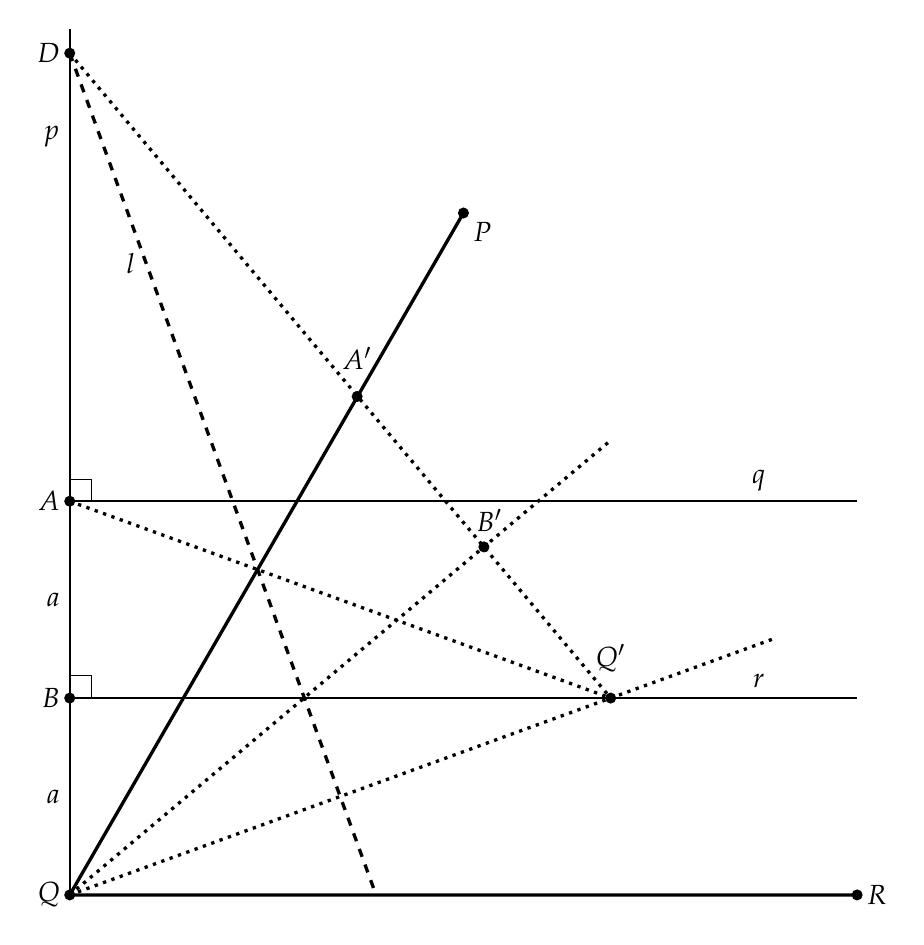
\begin{tikzpicture}[scale=1]

% Place points P, Q, R
\coordinate (P) at (60:10cm); %(5,8.67);
\coordinate (Q) at (0,0);
\coordinate (R) at (10,0);
\fill (P) circle (2pt) node[below right] {$P$};
\fill (Q) circle (2pt) node[left] {$Q$};
\fill (R) circle (2pt) node[right] {$R$};

% Draw PQR
\draw [very thick] (P)  -- (Q) -- (R);

% Draw perpendicular to QR
\draw [thick] (Q) -- node[left,very near end] {$p$} +(0,11);

% Draw parallel to QR and parallel halfway
\coordinate (A) at (0,5);
\coordinate (B) at (0,2.5);
\draw [thick] (A) -- node[above,very near end] {$q$} +(10,0);
\draw [thick] (B) -- node[above,very near end] {$r$} +(10,0);
\fill (A) circle (2pt) node[left] {$A$};
\fill (B) circle (2pt) node[left] {$B$};
\path (Q) -- node[left] {$a$} (B) -- node[left] {$a$} (A);
\draw (A) rectangle +(8pt,8pt);
\draw (B) rectangle +(8pt,8pt);

% Tangent line y = -2.75x + 10.69

% Draw fold
\coordinate (D) at (0,10.69);
\coordinate (fold-x) at (3.89,0);
\coordinate (AP) at (3.65,6.33);
\coordinate (QP) at (6.87,2.5);
\coordinate (BP) at (5.26,4.42);
\fill (D) circle (2pt) node[left] {$D$};
\fill (AP) circle (2pt) node[above,yshift=6pt] {$A'$};
\fill (QP) circle (2pt) node[above,yshift=6pt] {$Q'$};
\fill (BP) circle (2pt) node[above,xshift=2pt,yshift=2pt] {$B'$};
\draw [very thick,dashed] (D) -- node[left,near start] {$l$} (fold-x);

% Draw line of reflections
\draw [very thick, dotted] (D) -- (QP);

% Draw trisecting lines
\draw [very thick,dotted] (Q) -- ($(Q)!1.3!(QP)$);
\draw [very thick,dotted] (Q) -- ($(Q)!1.3!(BP)$);

% Complete triangle
\draw [very thick,dotted] (A) -- (QP);

\end{tikzpicture}
\end{center}
נתונה זווית חדה
$\angle PQR$,
יהי הקו
$p$
ניצב ל-%
$\overline{QR}$
ב-%
$Q$.
יהי הקו
$q$
ניצב ל-%
$p$
ב-% 
$A$
שחותך את
$\overline{PQ}$,
ויהי הקו
$r$
ניצב ל-%
$p$
ב-%
$B$
במחצית הדרך בן
$Q$
ו-%
$A$.

לפי אקסיומה 
$6$
בנה קיפול
$l$
המניח את 
$A$
על
$\overline{PQ}$ 
בנקודה
$A'$,
ומניח את
$Q$
על
$r$
בנקודה
$Q'$.
נסמן ב--%
$B'$
את השיקוף של 
$B$
מסביב ל-%
$l$.

בנה את הקווים
$\overline{QB'}$
ו-%
$\overline{QQ'}$.
טיעון: הזוויות
$\angle PQB'$, $\angle B'QQ'$, $\angle Q'QR$
מחלקות לשלושה חלקים את הזווית
$\angle PQR$.

\subsection{הוכחה ראשונה}

\begin{center}
\selectlanguage{english}
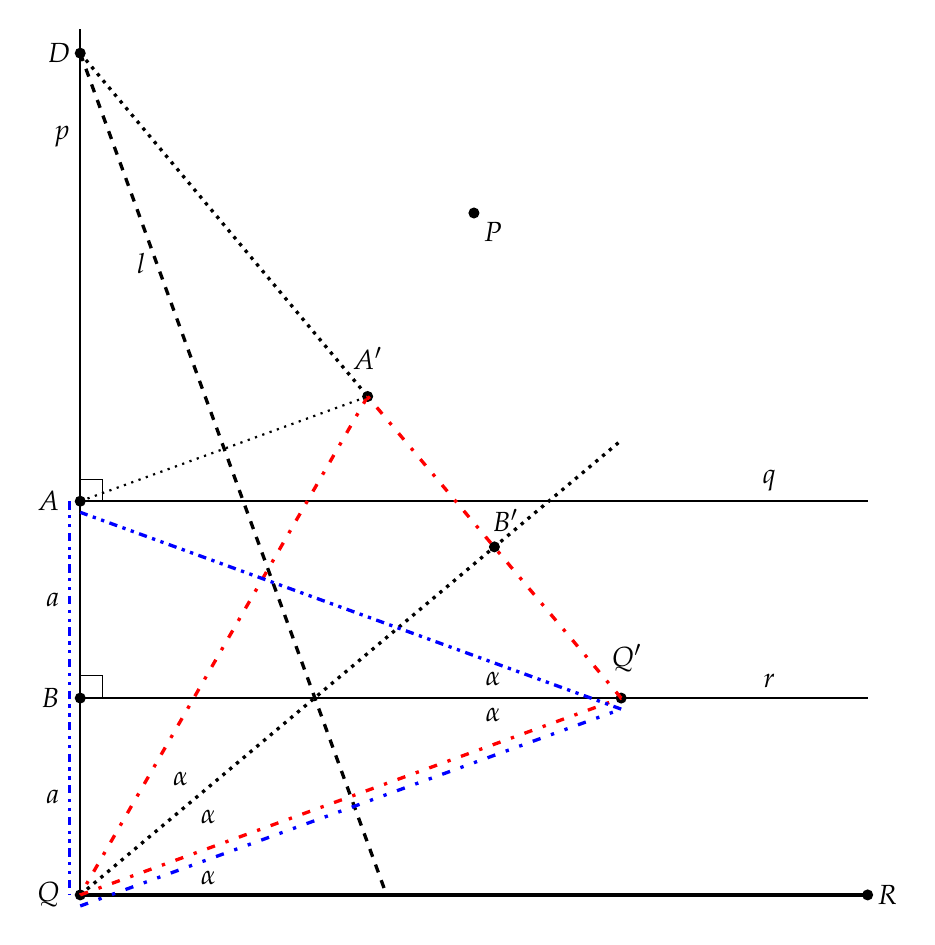
\begin{tikzpicture}[scale=1]

% Place points P, Q, R
\coordinate (P) at (60:10cm);
\coordinate (Q) at (0,0);
\coordinate (R) at (10,0);
\fill (P) circle (2pt) node[below right] {$P$};
\fill (Q) circle (2pt) node[left,xshift=-4pt] {$Q$};
\fill (R) circle (2pt) node[right] {$R$};

% Draw PQR
\draw [very thick] (Q) -- (R);

% Draw perpendicular to QR
\draw [thick] (Q) -- node[left,very near end] {$p$} +(0,11);

% Draw parallel to QR and parallel halfway
\coordinate (A) at (0,5);
\coordinate (B) at (0,2.5);
\draw [thick] (A) -- node[above,very near end] {$q$} +(10,0);
\draw [thick] (B) -- node[above,very near end] {$r$} +(10,0);
\fill (A) circle (2pt) node[left,xshift=-4pt] {$A$};
\fill (B) circle (2pt) node[left,xshift=-4pt] {$B$};
\path (Q) -- node[left,xshift=-4pt] {$a$} (B) -- node[left,xshift=-4pt] {$a$} (A);
\draw (A) rectangle +(8pt,8pt);
\draw (B) rectangle +(8pt,8pt);

% Tangent line y = -2.75x + 10.69

% Draw fold
\coordinate (D) at (0,10.69);
\coordinate (fold-x) at (3.89,0);
\coordinate (AP) at (3.65,6.33);
\coordinate (QP) at (6.87,2.5);
\coordinate (BP) at (5.26,4.42);
\fill (D) circle (2pt) node[left] {$D$};
\fill (AP) circle (2pt) node[above,yshift=6pt] {$A'$};
\fill (QP) circle (2pt) node[above,xshift=2pt,yshift=6pt] {$Q'$};
\fill (BP) circle (2pt) node[above,xshift=4pt,yshift=2pt] {$B'$};
\draw [very thick,dashed] (D) -- node[left,near start] {$l$} (fold-x);
	
% Draw line of reflections
\draw [very thick, dotted] (D) -- (AP);

% Draw trisecting lines
\draw [very thick,dotted] (Q) -- ($(Q)!1.3!(BP)$);

\draw [very thick,loosely dash dot,red] (Q) -- (QP);
\draw [very thick,loosely dash dot,red] (QP) -- (AP);
\draw [very thick,loosely dash dot,red] (AP) -- (Q);
\draw [very thick,loosely dash dot dot,blue] ($(Q)+(0,-4pt)$) -- ($(QP)+(0,-4pt)$);
\draw [very thick,dash dot dot,blue] ($(QP)+(0,-4pt)$) -- ($(A)+(0,-4pt)$);
\draw [very thick,dash dot dot,blue] ($(A)+(-4pt,0)$) -- ($(Q)+(-4pt,0)$);

\draw [thick,dotted] (A) -- (AP);

\node[left,xshift=-40pt,yshift=7pt] at (QP) {$\alpha$};
\node[left,xshift=-40pt,yshift=-6pt] at (QP) {$\alpha$};
\node[right,xshift=40pt,yshift=6pt] at (Q) {$\alpha$};
\node[right,xshift=40pt,yshift=28pt] at (Q) {$\alpha$};
\node[right,xshift=30pt,yshift=42pt] at (Q) {$\alpha$};

\end{tikzpicture}
\end{center}

הנקודות
$A', B', Q'$
הן שיקופים סביב אותו קו 
$l$
של הנקודות
$A,B,Q$
הנמצאות על קו אחד
$\overline{DQ}$,
ולכן גם הן נמצאות על קטע קו אחד
$\overline{DQ'}$.
לפי הבנייה,
$\overline{AB}=\overline{BQ}$, $\overline{BQ'}$
ניצב ל-%
$AQ$
ו-%
$\overline{BQ'}$
הוא צלע משותף, ולכן
$\triangle ABQ'\cong \triangle QBQ'$ 
לפי צלע-זווית-צלע. מכאן ש:
$\angle AQ'B=\angle QQ'B=\alpha$,
כי
$\overline{Q'B}$
הוא האנך האמצעי של המשולש שווי-שוקיים
$\triangle AQ'Q$.

לפי זוויות מתחלפות,
$\angle Q'QR=\angle QQ'B=\alpha$.

לפי שיקוף,
$\triangle AQ'Q\cong \triangle A'QQ'$.\footnote{%
שני המשולשים מודגשים על ידי קווים שונים של מקפים ונקודות, וכן על ידי הצבעים אדום וכחול.%
}
\begin{quote}
הוכחה: הקיפול
$l$
הוא האנך האמצעי של 
$\overline{AA'}$
וגם של
$\overline{QQ'}$;
בנה ניצבים מ-%
$A$
ו-%
$A'$
ל-%
$\overline{QQ'}$;
אזי
$\overline{AQ}=\overline{A'Q'}$
לפי משולשים ישר זווית חופפים.
$\overline{AA'Q'Q}$
הוא טרפז שווי-שוקיים כך שהאלכסונים שווים
$\overline{AQ'}=\overline{A'Q}$.
\end{quote}
מכאן ש-%
$\overline{QB'}$,
השיקוף של
$\overline{Q'B}$,
הוא האנך האמצעי של משולש שווי-שוקיים
$\triangle A'QQ'$,
ו-%
$\angle A'QB'=\angle Q'QB'=\angle QQ'B=\alpha$.

\subsection{הוכחה שנייה}

\begin{center}
\selectlanguage{english}
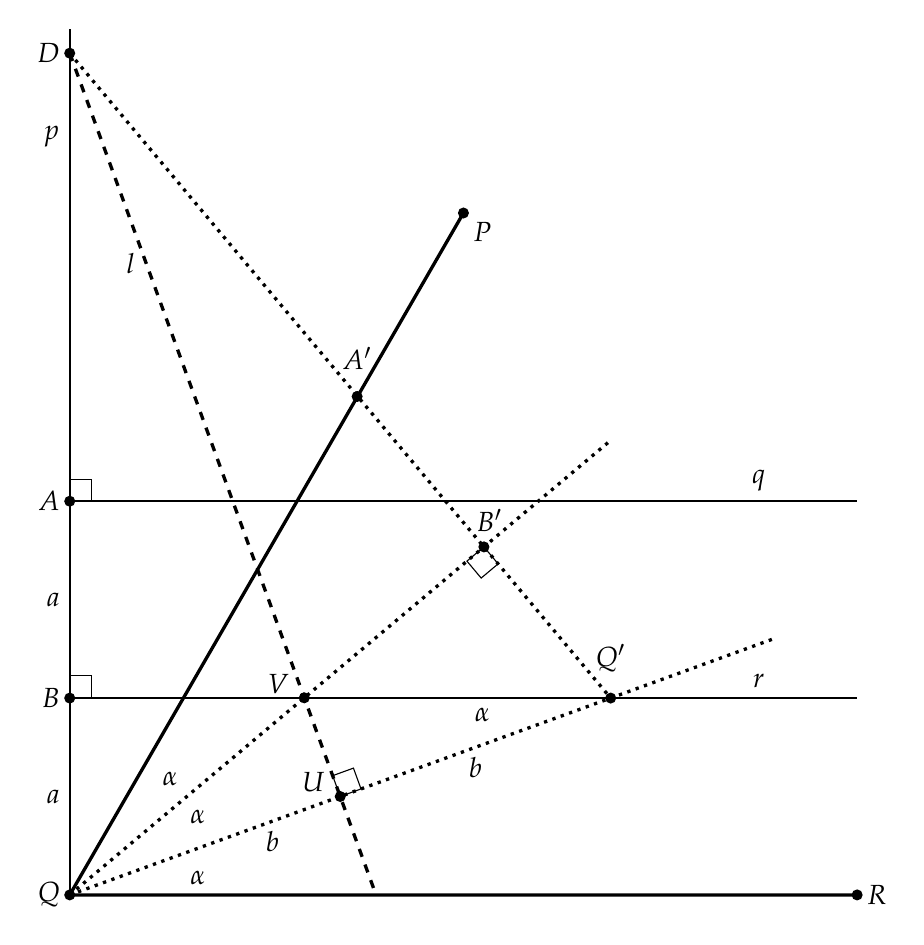
\begin{tikzpicture}[scale=1]

% Place points P, Q, R
\coordinate (P) at (60:10cm); %(5,8.67);
\coordinate (Q) at (0,0);
\coordinate (R) at (10,0);
\fill (P) circle (2pt) node[below right] {$P$};
\fill (Q) circle (2pt) node[left] {$Q$};
\fill (R) circle (2pt) node[right] {$R$};

% Draw PQR
\draw [very thick] (P)  -- (Q) -- (R);

% Draw perpendicular to QR
\draw [thick] (Q) -- node[left,very near end] {$p$} +(0,11);

% Draw parallel to QR and parallel halfway
\coordinate (A) at (0,5);
\coordinate (B) at (0,2.5);
\draw [thick] (A) -- node[above,very near end] {$q$} +(10,0);
\draw [thick] (B) -- node[above,very near end] {$r$} +(10,0);
\fill (A) circle (2pt) node[left] {$A$};
\fill (B) circle (2pt) node[left] {$B$};
\path (Q) -- node[left] {$a$} (B) -- node[left] {$a$} (A);
\draw (A) rectangle +(8pt,8pt);
\draw (B) rectangle +(8pt,8pt);

% Tangent line y = -2.75x + 10.69

% Draw fold
\coordinate (D) at (0,10.69);
\coordinate (fold-x) at (3.89,0);
\coordinate (AP) at (3.65,6.33);
\coordinate (QP) at (6.87,2.5);
\coordinate (BP) at (5.26,4.42);
\fill (D) circle (2pt) node[left] {$D$};
\fill (AP) circle (2pt) node[above,yshift=6pt] {$A'$};
\fill (QP) circle (2pt) node[above,yshift=6pt] {$Q'$};
\fill (BP) circle (2pt) node[above,xshift=2pt,yshift=2pt] {$B'$};
\draw [very thick,dashed,name path=fold] (D) -- node[left,near start] {$l$} (fold-x);

% Draw line of reflections
\draw [very thick, dotted] (D) -- (QP);

% Draw trisecting lines
\draw [very thick,dotted,name path=Qr] (Q) -- ($(Q)!1.3!(QP)$);
\draw [very thick,dotted,name path=Qq] (Q) -- ($(Q)!1.3!(BP)$);

% Draw indications of right angles
\draw[rotate=-140] (BP) rectangle +(8pt,8pt);
\path [name intersections = {of = fold and Qr, by = {U}}];
\fill (U) circle (2pt) node[above left,xshift=-2pt,yshift=-2pt] {$U$};
\draw[rotate=20] (U) rectangle +(8pt,8pt);
\path [name intersections = {of = fold and Qq, by = {V}}];
\fill (V) circle (2pt) node[above left,xshift=-2pt,yshift=-2pt] {$V$};

\path (Q) -- node[below,near end] {$b$} (U);
\path (U) -- node[below] {$b$} (QP);

\node[left,xshift=-40pt,yshift=-6pt] at (QP) {$\alpha$};
\node[right,xshift=40pt,yshift=6pt] at (Q) {$\alpha$};
\node[right,xshift=40pt,yshift=28pt] at (Q) {$\alpha$};
\node[right,xshift=30pt,yshift=42pt] at (Q) {$\alpha$};
\end{tikzpicture}
\end{center}

הקו
$l$
הוא קיפול, ולכן הוא האנך האמצעי של
$\overline{QQ'}$.
סמן ב-%
$U$
את נקודת החיתוך של
$l$
עם
$\overline{QQ'}$,
וסמן ב-%
$V$
את נקודת החיתוך שלו עם
$\overline{QB'}$.
$\triangle VUQ\cong \triangle VUQ'$
לפי צלע-זווית-צלע כי:
$\overline{VU}$
הוא צלע משותף, הזוויות ב-%
$U$
הן זוויות ישרות, ו-%
$\overline{QU}=\overline{Q'U}=b$.
מכאן ש-%
$\angle VQU=\angle VQ'U=\alpha$
ו-%
$\angle Q'QR=\angle VQ'U=\alpha$
לפי זוויות מתחלפות.

כמו בהוכחה הראשונה, הנקודות
$A', B', Q'$
הן כולן שיקופים סביב
$l$,
לכן הן כולן נמצאות על קטע קו אחד
$\overline{DQ'}$,
ו-%
$\overline{A'B'}=\overline{AB}=\overline{BQ}=\overline{B'Q'}=a$.
מכאן ש-%
$\triangle A'B'Q\cong\triangle Q'B'Q$
ו-%
$\angle A'QB'=\angle Q'QB'=\alpha$.


\newpage

\section{הבנייה של
\L{Martin}
לחלוקת זווית לשלושה חלקים%
}\label{s.tri2}

\subsection{הבנייה}

\begin{center}
\selectlanguage{english}
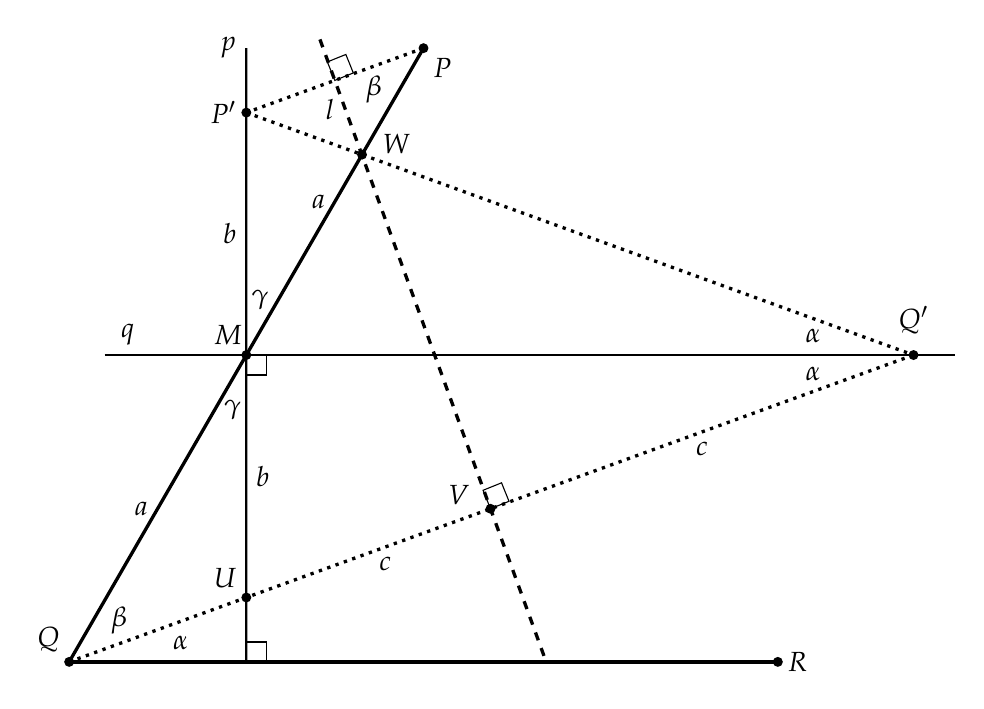
\begin{tikzpicture}[scale=.9]

% Place points P, Q, R
\coordinate (P) at (60:10cm); %(5,8.67);
\coordinate (Q) at (0,0);
\coordinate (R) at (10,0);
\fill (P) circle (2pt) node[below right] {$P$};
\fill (Q) circle (2pt) node[above left] {$Q$};
\fill (R) circle (2pt) node[right] {$R$};

% Draw PQR
\draw [very thick] (R)  -- (Q);
\draw [very thick,name path=pq] (Q) -- (P);

% M is the midpoint of PQ
\coordinate (M) at (2.5, 4.33);
\fill (M) circle (2pt) node[above left,xshift=2pt] {$M$};
\draw [rotate=-90] (M) rectangle +(8pt,8pt);

% Drop a perpendicular from M to QR and extend the line upwards
% This is the given line p
\coordinate (pQR) at (M |- Q);
\draw [thick,name path=p] (pQR) --
   node[left, very near end,yshift=28pt] {$p$}
   ($(pQR)!2!(M)$);
\draw (pQR) rectangle +(8pt,8pt);

% Construct q perpendicular to p through M
\draw [thick,name path=q] ($(M)+(-2,0)$) --
   node[above, very near start,xshift=-30pt] {$q$}
   ($(M)+(10,0)$);

% Construct the fold line t
% Its equation is y = -2.75x + 18.51, as obtained from Geogebra
\coordinate (t1) at (6.7,.085);
\coordinate (t2) at (3.5,8.89);
\draw [very thick,dashed,name path=t] (t1) --
   node[very near end,left] {$l$}
   (t2);

% Construct a perpendicular to t through P
\coordinate (perp-p) at ($(t1)!(P)!(t2)$);
\path [name path=perp-p] (P) -- ($(P)!2.5!(perp-p)$);

% Get its intersection with t denoted Pt
% and its intersection with p named PP
\path [name intersections = {of = t and perp-p, by = {Pt}}];
\path [name intersections = {of = p and perp-p, by = {PP}}];
\fill (PP) circle(2pt) node[left] {$P'$};
\draw [rotate=22] (Pt) rectangle +(8pt,8pt);

% Draw PT
\draw [very thick,dotted] (P) -- (PP);

% Construct a perpendicular to t through Q
\coordinate (perp-q) at ($(t1)!(Q)!(t2)$);
\path[name path=perp-q] (Q) -- ($(Q)!2.1!(perp-q)$);

% Get its intersection with t denoted V
% and its intersection with q denoted S=Q'
\path [name intersections = {of = t and perp-q, by = {V}}];
\path [name intersections = {of = q and perp-q, by = {QP}}];
\fill (QP) circle(2pt) node[above,yshift=4pt] {$Q'$};
\fill (V) circle(2pt) node[above left,xshift=-4pt,yshift=-2pt] {$V$};
\draw [rotate=22] (V) rectangle +(8pt,8pt);

% Draw Q QP
\draw [very thick,dotted,name path=qs] (Q) -- (QP);

% Get the intersection of QS with p denoted U
\path [name intersections = {of = p and qs, by = {U}}];
\fill (U) circle(2pt) node[above left] {$U$};

% Draw PP QP
\draw [very thick,dotted,name path=ts] (PP) -- (QP);

% Get its intersection with QP denoted W
\path [name intersections = {of = ts and pq, by = {W}}];
\fill (W) circle(2pt) node[right,xshift=4pt,yshift=4pt] {$W$};

% Label line segments
\path (P) -- node[left] {$a$} (M);
\path (M) -- node[left]  {$a$} (Q);
\path (PP) -- node[left]  {$b$} (M);
\path (M) -- node[right] {$b$} (U);
\path (Q) -- node[below,near end] {$c$} (V);
\path (V) -- node[below] {$c$} (QP);

% Label angles
\node [xshift=5pt,yshift=20pt]        at (M) {$\gamma$};
\node [xshift=-5pt,yshift=-20pt]      at (M) {$\gamma$};
\node [xshift=18pt,yshift=15pt]       at (Q) {$\beta$};
\node [xshift=-18pt,yshift=-15pt]     at (P) {$\beta$};
\node [left,xshift=-30pt,yshift=7pt]  at (QP) {$\alpha$};
\node [left,xshift=-30pt,yshift=-7pt] at (QP) {$\alpha$};
\node [right,xshift=34pt,yshift=7pt]  at (Q) {$\alpha$};
\end{tikzpicture}
\end{center}

נתונה זווית חדה
$\angle PQR$,
תהי
$M$
נקודת האמצע של
$\overline{PQ}$.
בנה
$p$
ניצב ל-%
$\overline{QR}$
העובר דרך
$M$
ובנה
$q$
ניצב ל-%
$p$
העובר דרך 
$M$.
$q$
מקביל ל-%
$\overline{QR}$.

לפי אקסיומה $6$, בנה קיפול
$l$
המניח את
$P$
ב-%
$P'$
על
$p$,
ומניח את
$Q$
ב-%
$Q'$
על
$q$.
ייתכן שקיים מספר קיפולים מתאימים; בחר את הקיפול החותך את
$\overline{PM}$.

בנה את קטעי הקו
$\overline{PP'}$
ו-%
$\overline{QQ'}$.
סמן ב-%
$U$
את נקודת החיתוך של
$\overline{QQ'}$
עם
$p$,
וסמן ב-%
$V$
את נקודת החיתוך שלו עם
$l$.
סמן ב-%
$W$
את החיתוכים של 
$\overline{PQ}$
ו-%
$\overline{P'Q'}$
עם
$l$.\footnote{%
לא ברור מאליו ש-%
$\overline{PQ}$
ו-%
$\overline{P'Q'}$
חותכים את
$l$
באותה נקודה. 
$\triangle PP'W\sim\triangle QQ'W$
כך שהגבהים מחלקים את הזוויות 
$\angle PWP', \angle QWQ'$
בצורה דומה וחייבים להיות על אותו קו.%
}

\subsection{הוכחה}

$\triangle QMU\cong \triangle PMP'$
לפי זווית-צלע-זווית:
$\angle P'PM=\angle UQM=\beta$
לפי זוויות מתחלפות;
$\overline{QM}=\overline{MP}=a$
כי 
$M$
היא נקודת האמצע של
$\overline{PQ}$;
$\angle QMU=\angle PMP'$
הן זוויות קודקודיות. מכאן ש-%
$\overline{P'M}=\overline{MU}=b$.

$\triangle P'MQ'\cong\triangle UMQ'$
לפי צלע-זוויות-צלע: הראנו ש-%
$\overline{P'M}=\overline{MU}=b$;
הזוויות ב-%
$M$
הן זוויות ישרות; 
$\overline{MQ'}$
הוא צלע משותף. הגובה של המשולש שווה-שוקיים 
$\triangle P'Q'U$ 
הוא חוצה הזווית
$\angle P'Q'U$
ולכן
$\angle P'Q'M=\angle UQ'M=\alpha$.


$\triangle QWV\cong\triangle Q'WV$
לפי צלע-זווית-צלע:
$\overline{QV}=\overline{VQ'}=c$
והזוויות ב-%
$V$
הן זוויות ישרות כי הקיפול הוא האנך אמצעי של
$\overline{QQ'}$; $\overline{VW}$
הוא צלע משותף. מכאן ש-%
$\angle WQV=\beta=\angle WQ'V=2\alpha$.
הראנו ש-%
$\angle PQR = \beta + \alpha = 2\alpha+\alpha=3\alpha$
ולכן
$\angle Q'QR$
היא שליש מ-%
$\angle PQR$.

% !TeX root = origami-math.tex

%%%%%%%%%%%%%%%%%%%%%%%%%%%%%%%%%%%%%%%%%%%%%%%%%%%%%%%%%%%%%%%%
\chapter{Doubling a Cube}\label{c.cube}

\section{Messer's doubling of a cube}\label{s.cube1}

A cube of volume $V$ has sides of length $\sqrt[3]{V}$. The volume of a cube with twice the volume is $2\cdot V$, so we need to construct the length $\sqrt[3]{2\cdot V}=\sqrt[3]{2}\cdot \sqrt[3]{V}$. If we can construct $\sqrt[3]{2}$, we can multiply by the given length $\sqrt[3]{V}$ to double the cube.

\subsection{Dividing a length into thirds}

Lang \cite{lang} shows efficient constructs for obtaining rational fractions of the length of the side of a square (piece of paper). Here, we need to divide the side of the square into thirds.

First, fold in half to locate the point $J=(1,1/2)$. Next, draw the lines $\overline{AC}$ and $\overline{BJ}$.
\begin{center}
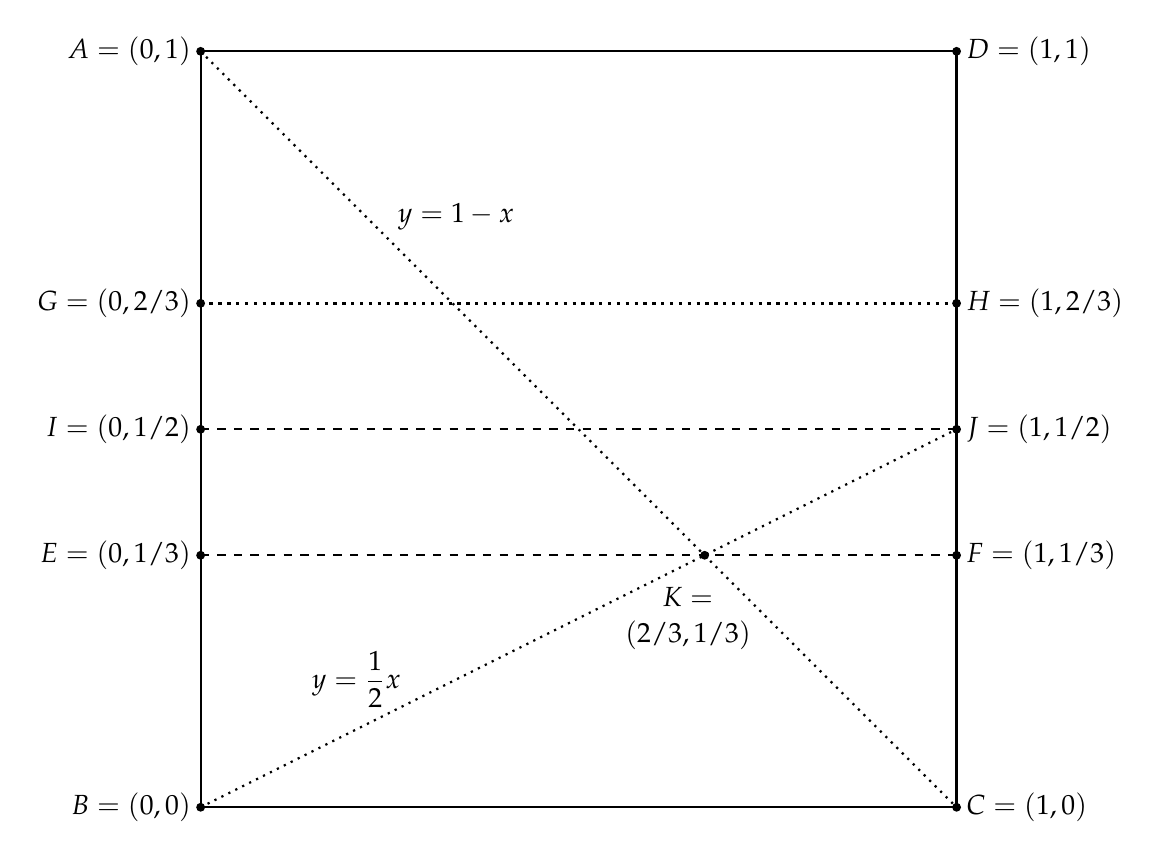
\begin{tikzpicture}[scale=.8]
% Draw square
\coordinate (A) at (0,12);
\coordinate (B) at (0,0);
\coordinate (C) at (12,0);
\coordinate (D) at (12,12);

\fill (A) circle (2pt) node[left]  {$A=(0,1)$};
\fill (B) circle (2pt) node[left]  {$B=(0,0)$};
\fill (C) circle (2pt) node[right] {$C=(1,0)$};
\fill (D) circle (2pt) node[right] {$D=(1,1)$};

\draw [thick] (A)  -- (B) -- (C) -- (D) -- cycle;

% Divide a side in half

\coordinate (M)  at (0,6);
\coordinate (N) at (12,6);
\fill (M) circle (2pt) node[left] {$I=(0,1/2)$};
\fill (N) circle (2pt) node[right] {$J=(1,1/2)$};
\draw [thick,dashed] (M) -- (N);


\draw [thick,dotted,name path=ac] (A) -- 
   node[near start,above,xshift=24pt] {$y=1-x$} (C);
\draw [thick,dotted,name path=be2] (B) -- 
   node[near start,above,xshift=-12pt,yshift=-2pt] {$y=\disfrac{1}{2}x$} (N);

\path [name intersections = {of = ac and be2, by = {I}}];
\fill (I) circle (2pt) 
   node[below,xshift=-6pt,yshift=-8pt] {$K=$}
   node[below,xshift=-6pt,yshift=-20pt] {$(2/3,1/3)$};

\coordinate (E)  at (0,4);
\coordinate (F) at (12,4);
\fill (E) circle (2pt) node[left] {$E=(0,1/3)$};
\fill (F) circle (2pt) node[right] {$F=(1,1/3)$};
\draw [thick,dashed] (E) -- (F);

\coordinate (G)  at (0,8);
\coordinate (H) at (12,8);
\fill (G) circle (2pt) node[left] {$G=(0,2/3)$};
\fill (H) circle (2pt) node[right] {$H=(1,2/3)$};
\draw [very thick,dotted] (G) -- (H);
\end{tikzpicture}
\end{center}

The coordinates of their point of intersection $K$ is obtained by solving the two equations:
\begin{form}{1.8}
y&=&1-x\\
y&=&\disfrac{1}{2}x\,.
\end{form}
The result is $x=2/3, y=1/3$.

Construct the line $\overline{EF}$ perpendicular to $\overline{AB}$ that goes $K$, and construct the reflection $\overline{GH}$ of $\overline{BC}$ around $\overline{EF}$. The side of the square has now been divided into thirds.

\subsection{Computing $\sqrt[3]{2}$}

\begin{center}
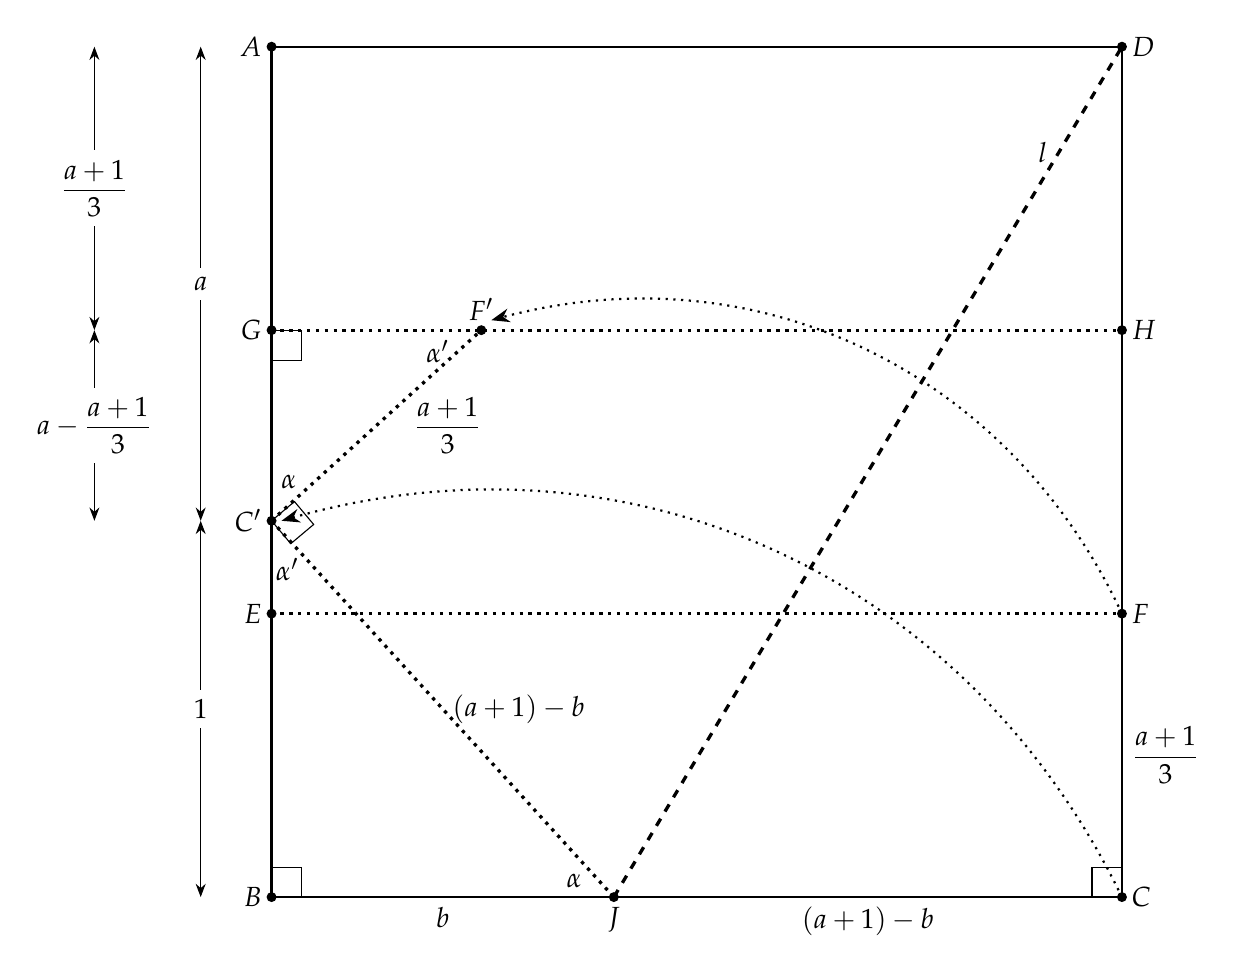
\begin{tikzpicture}[scale=.9]
% Draw and label square
\coordinate (A) at (0,12);
\coordinate (B) at (0,0);
\coordinate (C) at (12,0);
\coordinate (D) at (12,12);
\fill (A) circle (2pt) node[left]  {$A$};
\fill (B) circle (2pt) node[left]  {$B$};
\fill (C) circle (2pt) node[right] {$C$};
\fill (D) circle (2pt) node[right] {$D$};
\draw (B) rectangle +(12pt,12pt);
\draw[rotate=90] (C) rectangle +(12pt,12pt);
\draw [thick] (A)  -- (B) -- (C) -- (D) -- cycle;

% Draw line one-third from botton
\coordinate (E)  at (0,4);
\coordinate (F) at (12,4);
\fill (E) circle (2pt) node[left] {$E$};
\fill (F) circle (2pt) node[right] {$F$};
\draw [very thick,dotted,name path=ef] (E) -- (F);

% Draw line two-thirds from bottom
\coordinate (G)  at (0,8);
\coordinate (H) at (12,8);
\fill (G) circle (2pt) node[left] {$G$};
\fill (H) circle (2pt) node[right] {$H$};
\draw[rotate=-90] (G) rectangle +(12pt,12pt);
\draw [very thick,dotted] (G) -- (H);

% Draw reflections of C and F
\coordinate (CP) at (0,5.31);
\coordinate (FP) at (2.96,8);
\fill (CP) circle (2pt)
  node[left] {$C'$}
  node[above right,yshift=8pt] {$\alpha$}
  node[below right,xshift=-2pt,yshift=-10pt] {$\alpha'$};
\fill (FP) circle (2pt)
  node[above] {$F'$}
  node[below left,xshift=-8pt] {$\alpha'$};
\draw[rotate=-50] (CP) rectangle +(12pt,12pt);
\draw[very thick,dotted] (CP) -- (FP);

% Draw fold and fold arrows
% Tangent is y = 2.26x - 10.9
% Crosses x axis at (4.83,0)
\coordinate (J) at (4.83,0);
\fill (J) circle (2pt)
    node[below] {$J$}
    node[above left,xshift=-8pt] {$\alpha$};
\draw [very thick,dashed,name path=jd] (J) -- node[very near end,left] {$l$} (D);
\draw[thick,dotted,bend right=40,->] (C) to ($(CP)+(4pt,0)$);
\draw[thick,dotted,bend right=40,->] (F) to ($(FP)+(4pt,4pt)$);

% Draw hypotenuses of right triangles
\draw[very thick,dotted] (CP) -- (J);
\path (J)  -- (C);

% Labels on BC and hypotenuses
\path (CP) -- node[right] {$(a+1)-b$} (J);
\path (J)  -- node[below] {$(a+1)-b$} (C);
\path (B)  -- node[below] {$b$} (J);
\path (C)  -- node[right] {$\disfrac{a+1}{3}$} (F);
\path (CP) -- node[right,xshift=10pt] {$\disfrac{a+1}{3}$} (FP);

% Labels on AB
\draw[<->] ($(A)+(-1,0)$)    --
  node[fill=white] {$a$} ($(CP)+(-1,0)$);
\draw[<->] ($(CP)+(-1,0)$)   --
  node[fill=white] {$1$} ($(B)+(-1,0)$);
\draw[<->] ($(CP)+(-2.5,0)$) --
  node[fill=white] {$a-\disfrac{a+1}{3}$} ($(G)+(-2.5,0)$);
\draw[<->] ($(A)+(-2.5,0)$) --
  node[fill=white] {$\disfrac{a+1}{3}$} ($(G)+(-2.5,0)$);
\end{tikzpicture}
\end{center}

Label the side of the square by $a+1$. We will show that $a=\sqrt[3]{2}$.

Using Axiom~6 place $C$ at $C'$ on $\overline{AB}$ and $F$ at $F'$ on $\overline{GH}$.  Denote by $J$ the point intersection of the fold with $\overline{BC}$ and denote by $b$ the length of $\overline{BJ}$. The length of $\overline{JC}$ is $(a+1)-b$.

When the fold is performed, the line segment $\overline{JC}$ is reflected onto the line segment $\overline{C'J}$ of the same length, and $\overline{CF}$ is folded onto the line segment $\overline{C'F'}$ of the same length. A simple computation shows that the length of $\overline{GC'}$ is $a-\disfrac{a+1}{3}=\disfrac{2a-1}{3}$. Finally, since $\angle FCJ$ is a right angle, so is $\angle F'C'J$.

$\triangle C'BJ$ is a right triangle so by Pythagoras's theorem:
\begin{form}{1.3}
1^2 + b^2 &=& ((a+1)-b)^2\\
&=& a^2+2a+1 - 2(a+1)b + b^2\\
0&=&a^2+2a - 2(a+1)b\\
b&=&\disfrac{a^2+2a}{2(a+1)}\,.
\end{form}

$\angle GC'F' + \angle F'C'J + \angle JC'B = 180^\circ$ since they form the straight line $\overline{GB}$. Denote $\angle GC'F'$ by $\alpha$.
\[
\angle JC'B=180^\circ - \angle F'C'J - \angle GC'F'= 180^\circ - 90^\circ - \angle GC'F' = 90^\circ-\angle GC'F = 90^\circ -\alpha\,,
\]
which we denote by $\alpha'$. The triangles $\triangle C'BJ$, $\triangle F'GC'$ are right triangles, so $\angle C'JB=\alpha$ and $\angle C'F'G=\alpha'$. Therefore, the triangles are similar and we have:
\[
\disfrac{b}{(a+1)-b}=\disfrac{\disfrac{2a-1}{3}}{\disfrac{a+1}{3}}\,.
\]
Substituting for $b$:
\begin{form}{2}
\disfrac{\disfrac{a^2+2a}{2(a+1)}}{(a+1)-\disfrac{a^2+2a}{2(a+1)}}&=&\disfrac{2a-1}{a+1}\\
%\disfrac{a^2+2a}{(a+1)\cdot 2(a+1)-(a^2+2a)}&=&\disfrac{2a-1}{a+1}\\
\disfrac{a^2+2a}{a^2+2a +2}&=&\disfrac{2a-1}{a+1}\\
%a^3+3a^2+2a&=&(2a-1)(a^2+2a+2)\,.
%&=&2a^3+3a^2+2a-2\,.
\end{form}
Simplifying results in $a^3=2$, $a=\sqrt[3]{2}$.



\newpage

\section{Beloch's doubling of a cube}\label{s.cube2}

In 1936 Margharita P. Beloch was the first to formalize Axiom~6 (often called the \emph{Beloch fold}) and to show that it could be used to solve cubic equations. Here we give her construction for doubling the cube. The construction is treated in more detail in Chapters~\ref{c.lill}, \ref{c.beloch}.

\subsection{The construction}

Place point $A$ at $(-1,0)$ and point $B$ at $(0,-2)$. Let $p$ be the line with equation $x=1$ and let $q$ be the line with equation $y=2$.

Using Axiom~6 construct a fold $l$ that places $A$ at $A'$ on $p$ and $B$ at $B'$ on $q$. Denote the intersection of the fold and the $y$-axis by $X$ and the intersection of the fold and $x$-axis by $Y$.

\begin{center}
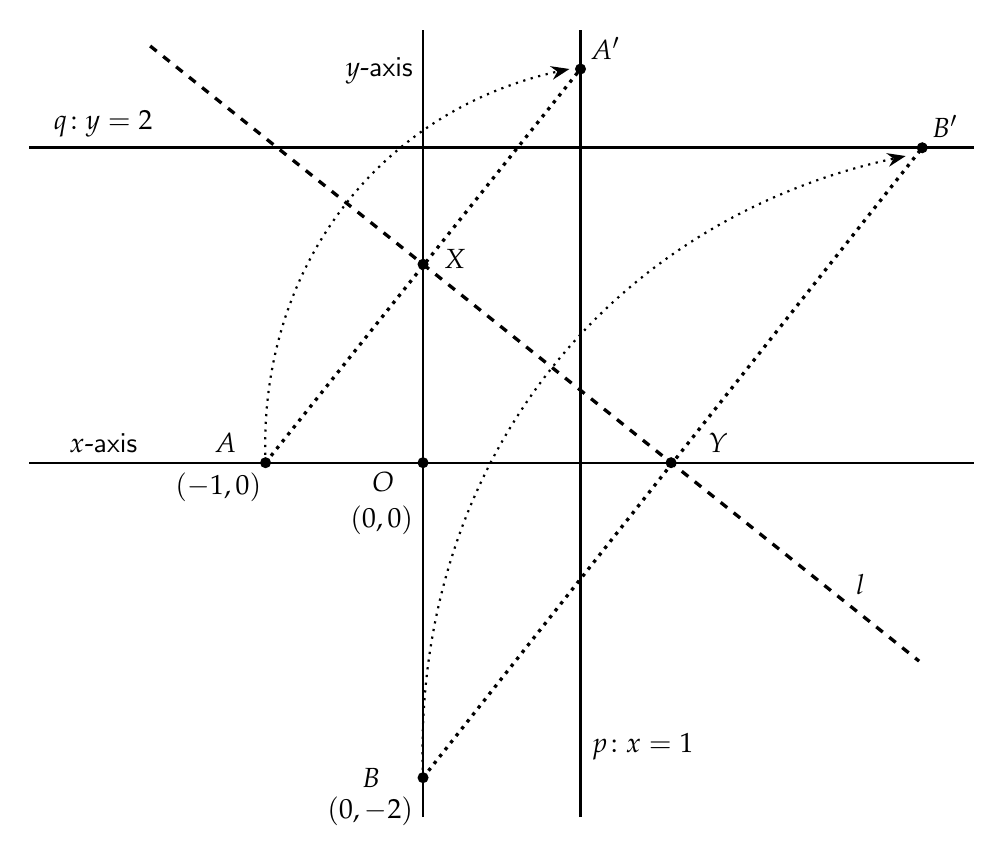
\begin{tikzpicture}[scale=1]
% Draw and label square
\coordinate (O) at (0,0);
\coordinate (A) at (-2,0);
\coordinate (B) at (0,-4);
\fill (O) circle (2pt)
  node[below left,xshift=-7pt] {$O$}
  node[below left,yshift=-12pt] {$(0,0)$};
\fill (A) circle (2pt)
  node[above left,xshift=-7pt] {$A$}
  node[below left,xshift=2pt,yshift=0pt] {$(-1,0)$};
\fill (B) circle (2pt)
  node[left,xshift=-12pt] {$B$}
  node[left,yshift=-12pt] {$(0,-2)$};

%\draw[thick] (0,-4.5) -- node[near start, left,yshift=-20pt] {$p$} +(0,10);
%\draw[thick] (-5,0) -- node[very near start, below,xshift=-16pt] {$q$} +(12,0);
\draw[thick] (0,-4.5) --  node[very near end,above left,yshift=12pt] {$y$-\textsf{axis}} +(0,10);
\draw[thick] (-5,0)   -- node[very near start,above left] {$x$-\textsf{axis}} +(12,0);
\draw[very thick] (2,-4.5) -- node[very near start, right,yshift=-10pt] {$p\!:x=1$} +(0,10);
\draw[very thick] (-5,4) -- node[very near start, above,xshift=-16pt] {$q\!: y=2$} +(12,0);

\coordinate (AP) at (2,5);
\fill (AP) circle (2pt) node[above right] {$A'$};
\coordinate (BP) at (6.34,4);
\fill (BP) circle (2pt) node[above right] {$B'$};

% Tangent y = -0.8x + 1.26

\coordinate (X) at (0,2.52);
\coordinate (Y) at (3.15,0);
\fill (X) circle (2pt) node[right,xshift=4pt,yshift=2pt] {$X$};
\fill (Y) circle (2pt) node[above right,xshift=10pt] {$Y$};
\draw [very thick,dashed] ($(X)!-1.1!(Y)$) -- node[very near end,right,xshift=8pt] {$l$} ($(X)!2!(Y)$);

\draw [very thick,dotted] (A) -- (AP);
\draw [very thick,dotted] (B) -- (BP);

\draw[thick,dotted,bend left=40,->] (A) to ($(AP)+(-4pt,0)$);
\draw[thick,dotted,bend left=40,->] (B) to ($(BP)+(-6pt,-3pt)$);

%\node[above left] at (0,4) {$(0,2)$};
%\node[below left] at (2,0) {$(1,0)$};

\end{tikzpicture}
\end{center}

\newpage

\subsection{Proof}

Let us extract a simplified diagram:

\begin{center}
\begin{tikzpicture}[scale=1]
\coordinate (O) at (0,0);
\coordinate (A) at (-2,0);
\coordinate (B) at (0,-4);
\fill (O) circle (2pt)
  node[below left,xshift=-7pt] {$O$};
\fill (A) circle (2pt)
  node[above left,xshift=-7pt] {$A$}
  node[above right,xshift=10pt] {$\alpha$};
\fill (B) circle (2pt)
  node[left,xshift=-12pt] {$B$}
  node[above right,yshift=12pt] {$\alpha'$};

\draw[thick] (0,-4.5) -- +(0,10);
\draw[thick] (-3,0)   -- +(8,0);

\coordinate (AP) at (2,5);
\fill (AP) circle (2pt) node[above right] {$A'$};
\coordinate (BP) at (6.34,4);
\fill (BP) circle (2pt) node[above right] {$B'$};

% Tangent y = -0.8x + 1.26

\coordinate (X) at (0,2.52);
\coordinate (Y) at (3.15,0);
\fill (X) circle (2pt)
  node[right,xshift=4pt,yshift=2pt] {$X$}
  node[below right,yshift=-14pt] {$\alpha$}
  node[below left,xshift=2pt,yshift=-12pt] {$\alpha'$};
\fill (Y) circle (2pt)
  node[above right,xshift=10pt] {$Y$}
  node[below left,xshift=-10pt] {$\alpha$}
  node[above left,xshift=-15pt] {$\alpha'$};
\draw [very thick,dashed] ($(X)!-.4!(Y)$) -- ($(X)!1.2!(Y)$);

\draw [very thick,dotted] (A) -- (AP);
\draw [very thick,dotted] (B) -- (BP);

\draw (0,0) rectangle +(10pt,10pt);
\draw[rotate=-130] (X) rectangle +(10pt,10pt);
\draw[rotate=-130] (Y) rectangle +(10pt,10pt);

\end{tikzpicture}
\end{center}

The fold is the perpendicular bisector of $\overline{AA'}$ and $\overline{BB'}$. Therefore, $\angle AXY$ and $\angle XYB$ are right angles and $\overline{AA'}$ is parallel to $\overline{BB'}$. By alternate interior angles $\angle XAO =\angle BYO=\alpha$. If an acute angle in a right triangle is $\alpha$, the other acute angle must be $90^\circ - \alpha$, which we denote $\alpha'$. The labeling of the angles in all the triangles in the diagram follows immediately.

We have three similar triangles $\triangle AOX\sim \triangle XOY \sim \triangle YOB$. $\overline{OA}=1$, $\overline{OB}=2$ are given, so:
\begin{form}{2}
\disfrac{\overline{OX}}{\overline{OA}}=\disfrac{\overline{OY}}{\overline{OX}}=\disfrac{\overline{OB}}{\overline{OY}}\\
\disfrac{\overline{OX}}{1}=\disfrac{\overline{OY}}{\overline{OX}}=\disfrac{2}{\overline{OY}}\\
\overline{OX}^2=\overline{OY}=\disfrac{2}{\overline{OX}}\;,
\end{form}
resulting in $\overline{OX}^3=2$ and $\overline{OX}=\sqrt[3]{2}$.

\documentclass[11pt,a4paper]{article}

%\usepackage[utf8x]{inputenc}

\usepackage{mathpazo}
\usepackage{microtype}
\usepackage{verbatim}
\usepackage{url}

\usepackage{tikz}
\usetikzlibrary{intersections,calc,through,arrows.meta}
\tikzset{>={Stealth[scale=1.4,inset=2pt]}}

\textwidth=155mm
\textheight=230mm
\topmargin=0pt
\headheight=0pt
\oddsidemargin=0mm
\evensidemargin=0mm
\headsep=0pt
\parindent=0pt
\renewcommand{\baselinestretch}{1.15}
\setlength{\parskip}{0.3\baselineskip plus 1pt minus 1pt}

\setcounter{tocdepth}{1}

\newcommand*{\disfrac}[2]{\displaystyle\frac{#1}{#2}}
\newcommand*{\sm}[1]{$\scriptstyle #1$}

\newenvironment{form}[1]{%
\begin{displaymath}%
\renewcommand{\arraystretch}{#1}%
\begin{array}{lcl}}%
{\end{array}%
\end{displaymath}%
}

\begin{document}
\thispagestyle{empty}

\begin{center}
\textbf{\LARGE Lill's Method}

\bigskip
\bigskip

\textbf{\Large Moti Ben-Ari}

\bigskip
\bigskip

\url{http://www.weizmann.ac.il/sci-tea/benari/}

\bigskip
\bigskip

Version 0.1

\bigskip
\end{center}


\begin{small}
\begin{center}
\copyright{}\ 2020 Moti Ben-Ari
\end{center}

This work is licensed under the Creative Commons Attribution-ShareAlike 3.0 Unported License. To view a copy of this license, visit \url{http://creativecommons.org/licenses/by-sa/3.0/} or send a letter to Creative Commons, 444 Castro Street, Suite 900, Mountain View, California, 94041, USA.
\end{small}

\newpage

\section{Magic}

Construct a path consisting of four line segments $\{a_3,a_2,a_1,a_0\}$ of lengths:
\[
\{a_3=1,a_2=6,a_1=11,a_0=6\}\,,
\]
starting from the origin, first along the $x$-axis and turning $90^\circ$ counterclockwise between segments. Construct a second path as follows: draw a line from the origin at an angle of $63.4^\circ$ and mark its intersection with $a_2$ by $P$. Turn left $90^\circ$, draw a line and and mark its intersection with $a_1$ by $Q$. Turn left $90^\circ$ once again, draw a line and note that it intersects the end of the first path at $(-10,0)$. %See Figure~\ref{fig.magic}.

%\begin{figure}[H]
\begin{center}
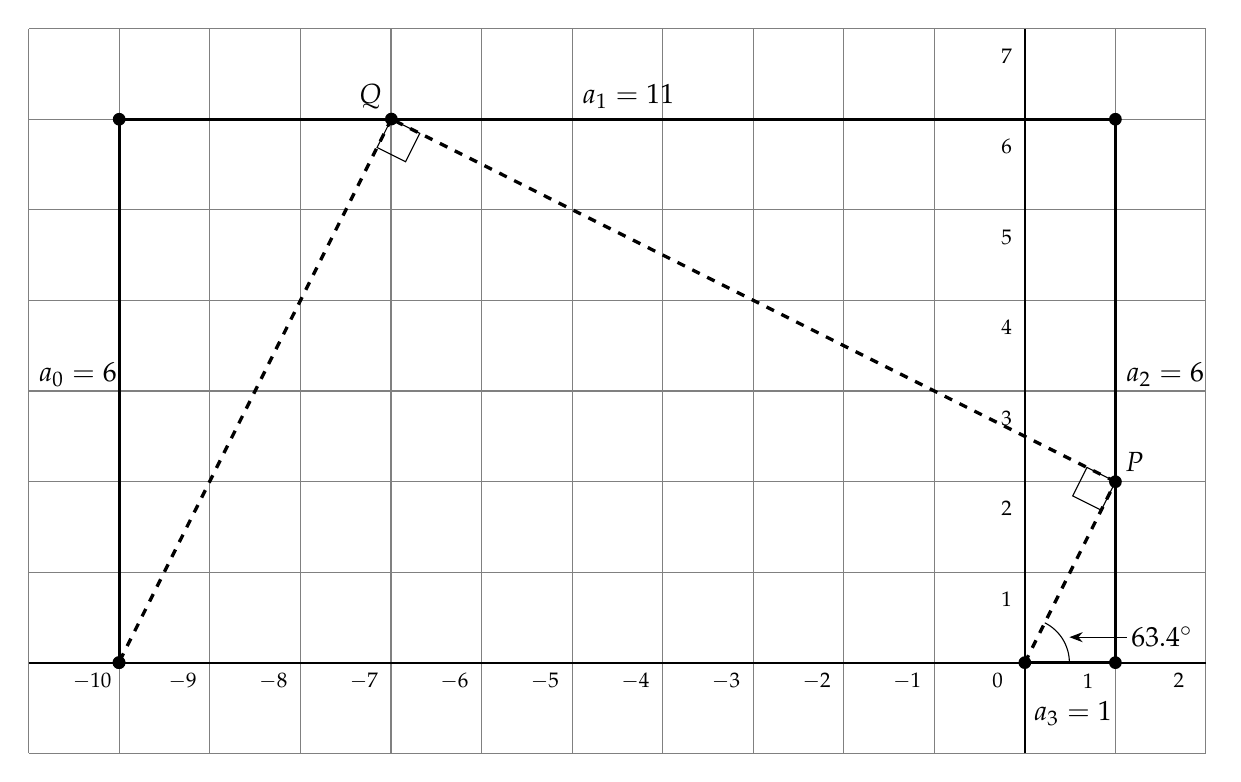
\begin{tikzpicture}[scale=1.15]
\draw[step=10mm,white!50!black] (-11,-1) grid (2,7);
\draw[thick] (-11,0) -- (2,0);
\draw[thick] (0,-1) -- (0,7);
\foreach \x in {-10,...,2}
  \node at (\x-.3,-.2) {\sm{\x}};
\foreach \y in {1,...,7}
  \node at (-.2,\y-.3) {\sm{\y}};
\coordinate (A) at (0,0);
\coordinate (B) at (1,0);
\coordinate (C) at (1,6);
\coordinate (D) at (-10,6);
\coordinate (E) at (-10,0);
\foreach \x in {A,B,C,D,E}
  \fill (\x) circle(2pt);
\draw[very thick] (A) --
  node[below,xshift=1pt,yshift=-10pt] {$a_3=1$} (B);
\draw[very thick,name path=bc] (B) -- 
  node[right,yshift=6pt] {$a_2=6$} (C);
\draw[very thick,name path=cd] (C) --
  node[above,xshift=4pt] {$a_1=11$}(D);
\draw[very thick,name path=de] (D) --
  node[left,xshift=3pt,yshift=6pt] {$a_0=6$}(E);

\path[name path=a2] (A) -- +(63.4:4);
\path [name intersections = {of = a2 and bc, by = {A2}}];
\fill (A2) circle(2pt) node[above right] {$P$};
\draw[very thick,dashed] (A) -- (A2);
\draw ($(A) + (14pt,0)$)
  arc [start angle=0, end angle = 63.4, radius=14pt];
\node[above right,xshift=35pt,yshift=2pt] at (A) {$63.4^\circ$};
\draw[->] ($(A)+(32pt,8pt)$) -- +(-18pt,0);
\draw[rotate=153.4] (A2) rectangle +(10pt,10pt);

\path[name path=b2] (A2) -- +(153.4:10);
\path [name intersections = {of = b2 and cd, by = {B2}}];
\fill (B2) circle(2pt) node[above left] {$Q$};
\draw[very thick,dashed] (A2) -- (B2);
\draw[rotate=243.4] (B2) rectangle +(10pt,10pt);

\path[name path=c2] (B2) -- +(243.4:7.5);
\path [name intersections = {of = c2 and de, by = {C2}}];
\fill (C2) circle(2pt);
\draw[very thick,dashed] (B2) -- (C2);
\end{tikzpicture}
\end{center}
%\caption{Magic}\label{fig.magic}
%\end{figure}
Let $p(x)=a_3x^+a_2x^2+a_1x+a_0=x^3+6x^2+11x+6$. Compute $\tan 63.4^\circ=2$, the tangent of the angle at the start of the first path. Then:
\[
p(-\tan 63.4^\circ)=(-2)^3+6(-2)^2+11(-2)+6=0\,.
\]
Congratulations! You have found a root of the cubic polynomial $x^3+6x^2+11x+6$.

\newpage

\section{Introduction}
This example demonstrates a method discovered by Eduard Lill in 1867 for graphically finding the real roots of any polynomial \cite{bradford, hull-beloch, riaz}. For simplicity, we limit our discussion here to cubic polynomials.

Clearly, this is not an algebraic method of computing roots of cubic equations; in the example, we are essentially verifying that $-2$ is a root. However, Lill's method has seen new interest because it can be implemented by origami \cite{hull-beloch} as we shall show in Section~\ref{s.origami}.

In Sections~\ref{s.multiple}--\ref{s.noroots} we continue the initial example to find additional roots of the polynomial and to show that if an angle $\alpha$ is chosen such that $-\tan\alpha$ is \emph{not} a root, then the construction doesn't work.

Section~\ref{s.method} presents the full specification of Lill's method. Some of the description may be difficult to understand, but will be clarified when demonstrated by additional examples in Sections~\ref{s.negative}, \ref{s.zero}, \ref{s.noninteger}. Since Lill's method can find a real root of any cubic polynomial, it can be used to trisect an angle. In particular, since it can find $\sqrt[3]{2}$, the root of $x^3-2$, it can double a cube as shown in Section~\ref{s.cube}.

Section~\ref{s.proof} gives a proof that Lill's method can find the real roots of any cubic polynomial. The proof for arbitrary polynomials follows the same structure.

Section~\ref{s.origami} investigates the connection between Lill's method and origami.

\newpage

\section{Multiple roots}\label{s.multiple}

Let us continue the example above. The polynomial $p(x)=a_3x^3+6x^2+11x+6$ has three roots $-1,-2,-3$. Computing the arc tangent of the negation of the roots gives:
\[
\tan^{-1} = 45^\circ,\; -\tan^{-1} = 63.4^\circ,\; \tan^{-1} = 71.6^\circ\,.
\]
%In Figure~\ref{fig.multiple} 
In the diagram below we see that for each of the three angles, the second path intersects the end of the first path.
%\begin{figure}[htb]
\begin{center}
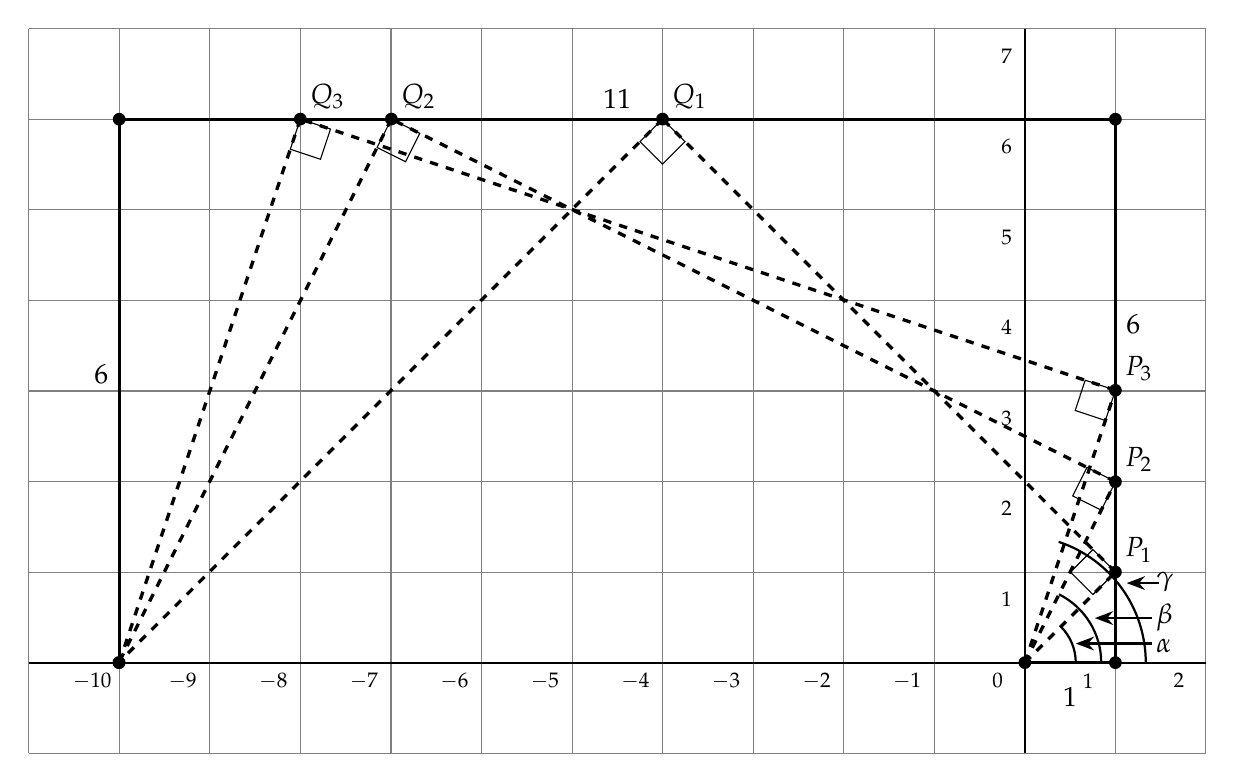
\begin{tikzpicture}[scale=1.15]
\draw[step=10mm,white!50!black] (-11,-1) grid (2,7);
\draw[thick] (-11,0) -- (2,0);
\draw[thick] (0,-1) -- (0,7);
\foreach \x in {-10,...,2}
  \node at (\x-.3,-.2) {\sm{\x}};
\foreach \y in {1,...,7}
  \node at (-.2,\y-.3) {\sm{\y}};
\coordinate (A) at (0,0);
\coordinate (B) at (1,0);
\coordinate (C) at (1,6);
\coordinate (D) at (-10,6);
\coordinate (E) at (-10,0);
\foreach \x in {A,B,C,D,E}
  \fill (\x) circle(2pt);
\draw[very thick] (A) -- node[below,yshift=-5pt] {$1$} (B);
\draw[very thick,name path=bc] (B) -- 
  node[right,yshift=24pt] {$6$} (C);
\draw[very thick,name path=cd] (C) --
  node[above] {$11$}(D);
\path[name path=de] (D) -- ($(E)+(0,-.8)$);
\draw[very thick] (D) --
  node[left,yshift=6pt] {$6$} (E);

\path[name path=a2] (A) -- +(63.4:4);
\path [name intersections = {of = a2 and bc, by = {A2}}];
\fill (A2) circle(2pt);
\draw[very thick,dashed] (A) -- (A2);
\draw[thick] ($(A) + (24pt,0)$)
  arc [start angle=0, end angle = 63.4, radius=24pt];
\node[above right,xshift=44pt,yshift=8pt] at (A) {$\beta$};
\draw[rotate=153.4] (A2) rectangle +(10pt,10pt);
\draw[Stealth-,thick] ($(A) + (22pt,14pt)$) -- +(18pt,0);

\path[name path=b2] (A2) -- +(153.4:10);
\path [name intersections = {of = b2 and cd, by = {B2}}];
\fill (B2) circle(2pt);
\draw[very thick,dashed] (A2) -- (B2);
\draw[rotate=243.4] (B2) rectangle +(10pt,10pt);

\path[name path=c2] (B2) -- +(243.4:7.5);
\path [name intersections = {of = c2 and de, by = {C2}}];
\fill (C2) circle(2pt);
\draw[very thick,dashed] (B2) -- (C2);

\path[name path=a1] (A) -- +(45:3);
\path [name intersections = {of = a1 and bc, by = {A1}}];
\fill (A1) circle(2pt);
\draw[very thick,dashed] (A) -- (A1);
\draw[thick] ($(A) + (16pt,0)$)
  arc [start angle=0, end angle = 45, radius=16pt];
\node[above right,xshift=44pt,yshift=0pt] at (A) {$\alpha$};
\draw[rotate=135] (A1) rectangle +(10pt,10pt);
\draw[Stealth-,thick] ($(A) + (16pt,6pt)$) -- +(24pt,0);

\path[name path=b1] (A1) -- +(135:8);
\path [name intersections = {of = b1 and cd, by = {B1}}];
\fill (B1) circle(2pt);
\draw[very thick,dashed] (A1) -- (B1);
\draw[rotate=225] (B1) rectangle +(10pt,10pt);

\path[name path=c1] (B1) -- +(225:9);
\path [name intersections = {of = c1 and de, by = {C1}}];
%\fill (C1) circle(2pt);
\draw[very thick,dashed] (B1) -- (C1);

\path[name path=a3] (A) -- +(71.6:4);
\path [name intersections = {of = a3 and bc, by = {A3}}];
\fill (A3) circle(2pt);
\draw[very thick,dashed] (A) -- (A3);
\draw[thick] ($(A) + (38pt,0)$)
  arc [start angle=0, end angle = 71.6, radius=40pt];
\node[above right,xshift=44pt,yshift=22pt] at (A) {$\gamma$};
\draw[rotate=161.6] (A3) rectangle +(10pt,10pt);
\draw[Stealth-,thick] ($(A) + (32pt,25pt)$) -- +(10pt,0);

\path[name path=b3] (A3) -- +(161.6:10);
\path [name intersections = {of = b3 and cd, by = {B3}}];
\fill (B3) circle(2pt);
\draw[very thick,dashed] (A3) -- (B3);
\draw[rotate=251.6] (B3) rectangle +(10pt,10pt);

\path[name path=c3] (B3) -- +(251.6:7);
\path [name intersections = {of = c3 and de, by = {C3}}];
%\fill (C3) circle(2pt);
\draw[very thick,dashed] (B3) -- (C3);

\node[above right] at (A1) {$P_1$};
\node[above right] at (A2) {$P_2$};
\node[above right] at (A3) {$P_3$};
\node[above right] at (B1) {$Q_1$};
\node[above right] at (B2) {$Q_2$};
\node[above right] at (B3) {$Q_3$};
\end{tikzpicture}
\end{center}
%\caption{Multiple roots}\label{fig.multiple}
%\end{figure}

\newpage

\section{Paths that do not lead to roots}\label{s.noroots}

Perhaps the second path intersects the end of the first path for \emph{any} initial angle, for example, $56.3^\circ$. The second path intersects the extension of the line segment $a_0$, but not at $(-10,0)$, the end of the first path.
% (Figure~\ref{fig.noroots}).
We conclude that $-\tan 56.3=-1.5$ is \emph{not} a root of the equation.
%\begin{figure}[htb]
\begin{center}
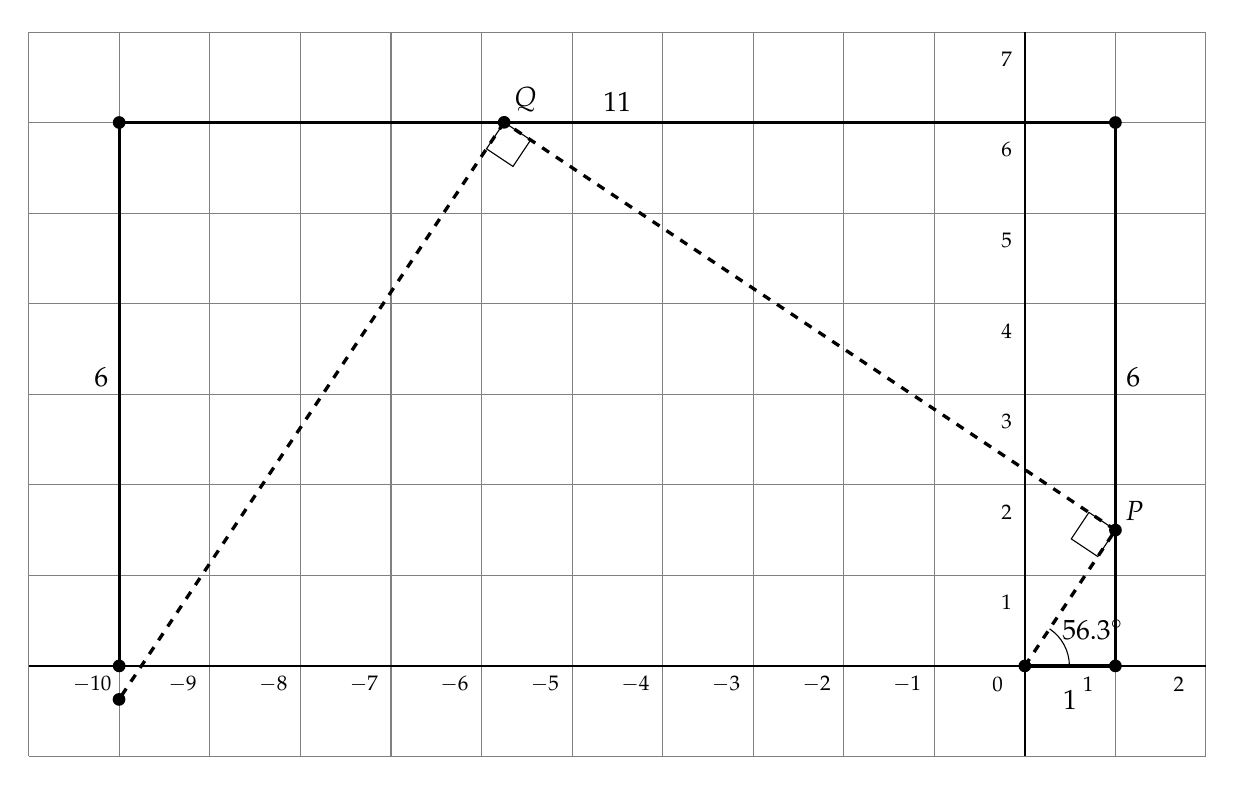
\begin{tikzpicture}[scale=1.15]
\draw[step=10mm,white!50!black] (-11,-1) grid (2,7);
\draw[thick] (-11,0) -- (2,0);
\draw[thick] (0,-1) -- (0,7);
\foreach \x in {-10,...,2}
  \node at (\x-.3,-.2) {\sm{\x}};
\foreach \y in {1,...,7}
  \node at (-.2,\y-.3) {\sm{\y}};
\coordinate (A) at (0,0);
\coordinate (B) at (1,0);
\coordinate (C) at (1,6);
\coordinate (D) at (-10,6);
\coordinate (E) at (-10,0);
\foreach \x in {A,B,C,D,E}
  \fill (\x) circle(2pt);
\draw[very thick] (A) -- node[below,yshift=-5pt] {$1$} (B);
\draw[very thick,name path=bc] (B) -- 
  node[right,yshift=6pt] {$6$} (C);
\draw[very thick,name path=cd] (C) --
  node[above] {$11$}(D);
\draw[very thick] (D) --
  node[left,yshift=6pt] {$6$}(E);
\path[name path=de] (-10,-1) -- (-10,7);

\path[name path=a2] (A) -- +(56.3:3);
\path [name intersections = {of = a2 and bc, by = {A2}}];
\fill (A2) circle(2pt);
\draw[very thick,dashed] (A) -- (A2);
\draw ($(A) + (14pt,0)$)
  arc [start angle=0, end angle = 56.3, radius=14pt];
\node[above right,xshift=10pt,yshift=6pt] at (A) {$56.3^\circ$};
\draw[rotate=146.3] (A2) rectangle +(10pt,10pt);

\path[name path=b2] (A2) -- +(146.3:10);
\path [name intersections = {of = b2 and cd, by = {B2}}];
\fill (B2) circle(2pt);
\draw[very thick,dashed] (A2) -- (B2);
\draw[rotate=236.3] (B2) rectangle +(10pt,10pt);

\path[name path=c2] (B2) -- +(236.3:8.5);
\path [name intersections = {of = c2 and de, by = {C2}}];
\fill (C2) circle(2pt);
\draw[very thick,dashed] (B2) -- (C2);

\node[above right] at (A2) {$P$};
\node[above right] at (B2) {$Q$};
\end{tikzpicture}
\end{center}
%\caption{$56.3^\circ$ is not a root}\label{fig.noroots}
%\end{figure}

\newpage

\section{Specification of Lill's method}\label{s.method}

This section gives the complete specification of Lill's method for finding real roots of cubic polynomials. Examining the examples below will help understand the details.
\begin{itemize}
\item Start with an arbitrary cubic polynomial: $p(x)=a_3x^3+a_2x^2+a_1x+a_0$.
\item Construct the first path as follows:
\begin{itemize}
\item For each coefficient $a_3,a_2,a_1,a_0$ (in that order) draw a line segment starting at the origin $O=(0,0)$ in the positive direction of the $x$-axis. Turn $90^\circ$ counterclockwise between each segment.
\end{itemize}
\item Construct the second path as follows:
\begin{itemize}
\item We use $a_i$ to denote the side of length $a_i$.
\item Construct a line from $O$ at an angle of $\theta$ with the positive $x$-axis that intersects $a_2$ at point $P$.
\item Turn $\pm 90^\circ$ and construct a line from $P$ that intersects $a_1$ at $Q$.
\item Turn $\pm 90^\circ$ and construct a line from $Q$ that intersects $a_0$ at $R$.
\item If $R$ is the end point of the first path, then $-\tan\theta$ is a root of $p(x)$.
\end{itemize}
\item Special cases:
\begin{itemize}
\item When drawing the line segments of the first path, if a coefficient is negative, draw the line segment \emph{backwards}.
\item When drawing the line segments of the first path, if a coefficient is zero, do not draw a line segment but continue with the next $\pm90^\circ$ turn.
\end{itemize}
\item Notes:
\begin{itemize}
\item "Intersects $a_i$" includes ``intersects with the line that contains $a_i$''.
\item When building the second path, choose to turn left or right by $90^\circ$ so that there is an intersection with the next segment of the first path.
\end{itemize}
\end{itemize}

\newpage

\section{Negative coefficients}\label{s.negative}

In \cite{moti-origami} I gave an example of the use of origami Axiom~6 which results in the polynomial $p(x)=x^3-3x^2-3x+1$ which has negative coefficients.

We start by drawing a segment of length $1$ to the right. Next we turn $90^\circ$ to face up, but the coefficient is negative, so we draw a segment of length $3$ \emph{down}. After turning $90^\circ$ to the left, the coefficient is again negative, so we draw a segment of length $3$ to the right. Finally, we turn down and draw a segment of length $1$.

We start the second path with a line angled $45^\circ$ with the $x$-axis. It intersects the \emph{extension} of the vertical segment of length $-3$ at $(1,1)$. Turning $-90^\circ$ (to the right), the line intersects the \emph{extension} of the horizontal segment of length $-3$  at $(5,-3)$. Turning $-90^\circ$ again, the line intersects the end of the first path at $(4,-4)$.

Since $-\tan 45^\circ=-1$, a real root of the polynomial is $-1$:
\[
p(-1)=(-1)^3-3(-1)^2-3(-1)+6=-1-3+3+1=0\,.
\]
The loosely dashed lines in the Figure will be discussed  in Section~\ref{s.noninteger}.

\begin{center}
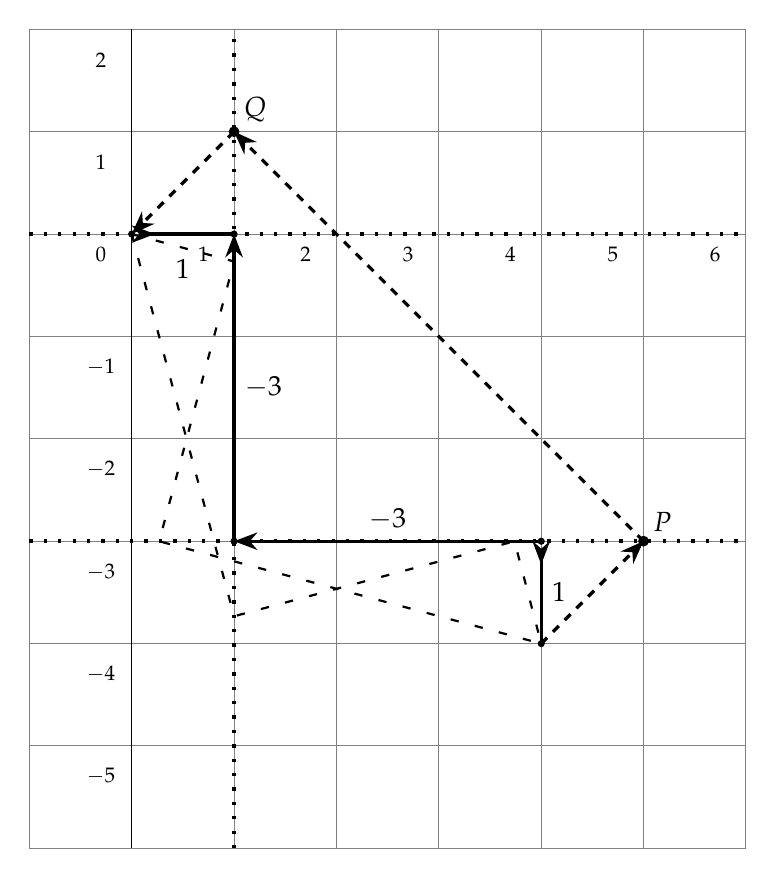
\begin{tikzpicture}[scale=1.3]
\draw[step=10mm,white!50!black] (-1,-6) grid (6,2);
%\draw (-1,0) -- (6,0);
\draw (0,-6) -- (0,2);
\foreach \x in {0,...,6}
  \node at (\x-.3,-.2) {\sm{\x}};
\foreach \y in {-5,...,-1}
  \node at (-.3,\y-.3) {\sm{\y}};
\foreach \y in {1,...,2}
  \node at (-.3,\y-.3) {\sm{\y}};
\coordinate (A) at (0,0);
\coordinate (B) at (1,0);
\coordinate (C) at (1,-3);
\coordinate (D) at (4,-3);
\coordinate (E) at (4,-4);
\foreach \x in {A,B,C,D,E}
  \fill (\x) circle(1pt);
\draw[very thick,>-] (A) -- node[below,yshift=-5pt] {$1$} (B);
\draw[very thick,<-,name path=bc] (B) -- 
  node[right] {$-3$} (C);
\draw[very thick,<-,name path=cd] (C) --
  node[above] {$-3$}(D);
\draw[very thick,>-,name path=de] (D) --
  node[right] {$1$}(E);

\draw[very thick,loosely dotted,name path=a] (-1,0) -- (6,0);
\draw[very thick,loosely dotted,name path=b] (1,-6) -- (1,2);
\draw[very thick,loosely dotted,name path=c] (-1,-3) -- (6,-3);

\draw[very thick,dashed,-Stealth] (4,-4) -- (5,-3) coordinate (A2);
\fill (5,-3) circle (1.5pt) node[above right] {$P$};
\draw[very thick,dashed,-Stealth] (5,-3) -- (1,1) coordinate (B2);
\fill (1,1) circle (1.5pt) node[above right] {$Q$};
\draw[very thick,dashed,-Stealth] (1,1) -- (0,0);

\path[name path=a1] (A) -- +(-75:5);
\path [name intersections = {of = a1 and b, by = {B1}}];
\path[name path=b1] (B1) -- +(15:5);
\path [name intersections = {of = b1 and c, by = {C1}}];
\draw[thick,loosely dashed] (A) -- (B1) -- (C1) -- (E);

\path[name path=a3] (A) -- +(-15:5);
\path [name intersections = {of = a3 and b, by = {B3}}];
\path[name path=b3] (B3) -- +(-105:5);
\path [name intersections = {of = b3 and c, by = {C3}}];
\draw[thick,loosely dashed] (A) -- (B3) -- (C3) -- (E);
\end{tikzpicture}
\end{center}

\newpage

\section{Zero coefficients}\label{s.zero}

The coefficient of the $x^2$ term in the polynomial $x^3-7x-6=0$ is zero. 
For a term of the form $0\cdot x^2$, we draw a line segment of length $0$, that is, we do not draw a line, but we still make the $\pm 90^\circ$ turn before ``drawing'' it, as indicated by the arrow pointed up at point $(1,0)$ in the diagram. Next make an additional turn and draw a line of length $-7$, that is, of length $7$ backwards, to point $(8,0)$. Finally, turn again and draw a line of length $-6$ to point $(8,6)$.

There are three second paths that intersect the end of the first path. They start with angles of:
\[
\alpha=45^\circ,\; \beta=63.4^\circ,\; \gamma=-71.6^\circ\,.
\]
We conclude that there are three real roots:
\[
-\tan 45^\circ=-1,\; -\tan 63.4^\circ =-2,\; -\tan -71.6^\circ=3\,.
\]
Check:
\begin{form}{1.1}
(x+1)(x+2)(x-3)&=&(x^2+3x+2)(x-3)\\
%&=&x^3+3x^2+2x-3x^2-9x-6\\
&=&x^3-7x-6\,.
\end{form}

\begin{center}
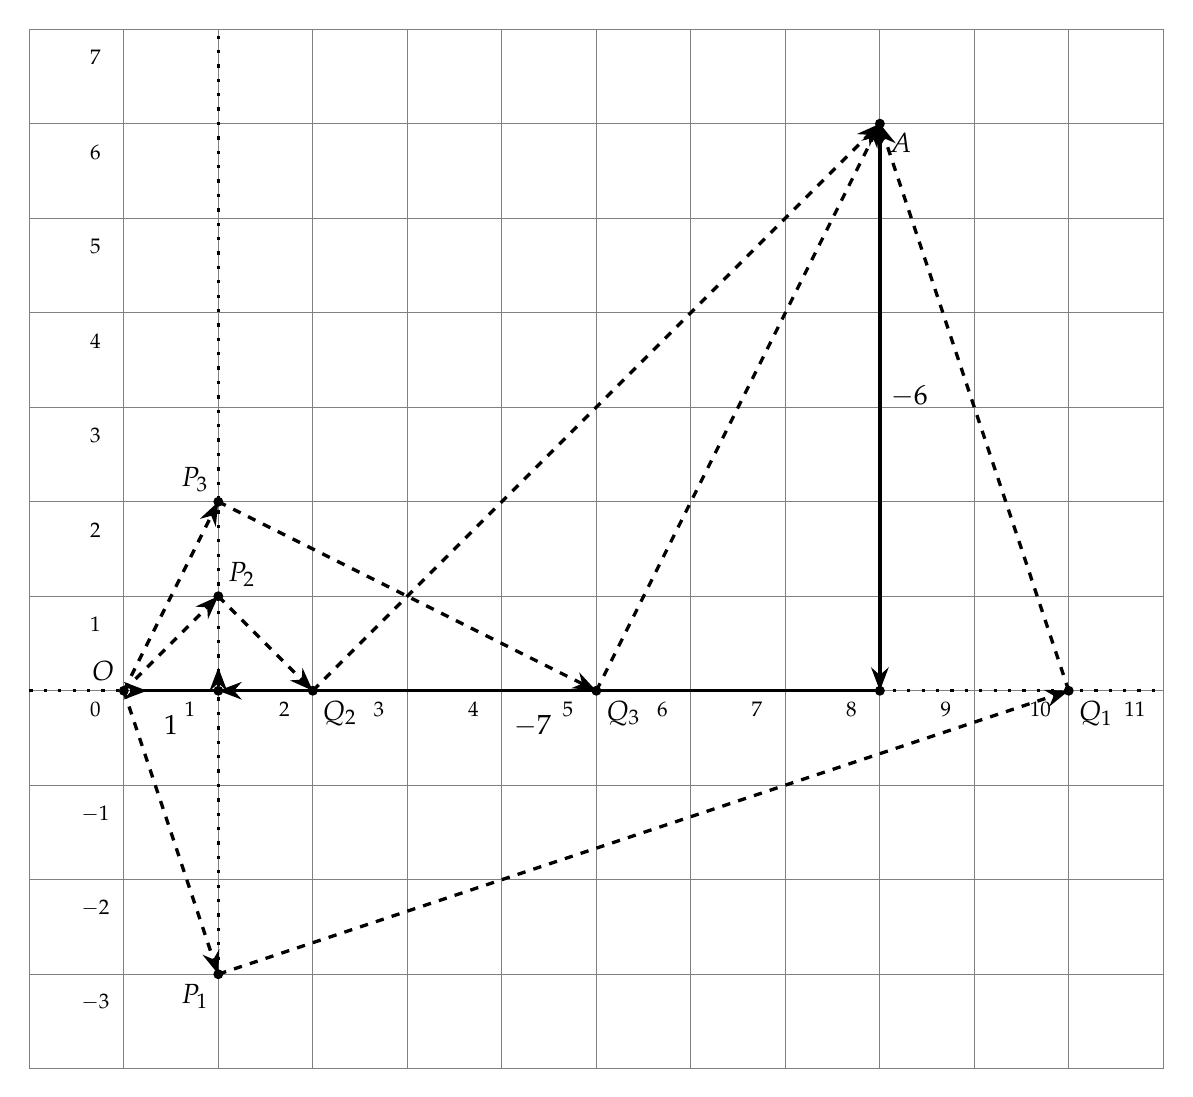
\begin{tikzpicture}[scale=1.2]
\draw[step=10mm,white!50!black] (-1,-4) grid (11,7);
%\draw (-1,0) -- (6,0);
%\draw (0,-6) -- (0,2);
\foreach \x in {0,...,11}
  \node at (\x-.3,-.2) {\sm{\x}};
\foreach \y in {-3,...,-1}
  \node at (-.3,\y-.3) {\sm{\y}};
\foreach \y in {1,...,7}
  \node at (-.3,\y-.3) {\sm{\y}};
\coordinate (A) at (0,0);
\node[above left] at (A) {$O$};
\coordinate (B) at (1,0);
\coordinate (C) at (8,0);
\coordinate (D) at (8,6);
\node[below right] at (D) {$A$};
\foreach \x in {A,B,C,D}
  \fill (\x) circle(1.5pt); 
\draw[very thick,>-] (A) -- node[below,yshift=-5pt] {$1$} (B);
\draw[>-,very thick] (B) -- ($(B)+(0,.1)$);
\draw[very thick,<-,name path=bc] (B) -- 
  node[below,xshift=-6pt,yshift=-5pt] {$-7$} (C);
\draw[very thick,<-,name path=cd] (C) --
  node[right,yshift=4pt] {$-6$}(D);
\draw[very thick,loosely dotted] (1,-3) -- (1,7);
\draw[very thick,loosely dotted] (-1,0) -- (11,0);

\draw[very thick,dashed,-Stealth] (0,0) -- (1,1) coordinate (A2);
\fill (A2) circle (1.5pt);
\draw[very thick,dashed,-Stealth] (A2) -- (2,0) coordinate (B2);
\fill (B2) circle (1.5pt);
\draw[very thick,dashed,-Stealth] (B2) -- (D);

\draw[very thick,dashed,-Stealth] (0,0) -- (1,2) coordinate (A3);
\fill (A3) circle (1.5pt);
\draw[very thick,dashed,-Stealth] (A3) -- (5,0) coordinate (B3);
\fill (B3) circle (1.5pt);
\draw[very thick,dashed,-Stealth] (B3) -- (D);

\draw[very thick,dashed,-Stealth] (0,0) -- (1,-3);
\fill (1,-3) circle (1.5pt);
\draw[very thick,dashed,-Stealth] (1,-3) coordinate (A1) -- (10,0);
\fill (10,0) circle (1.5pt);
\draw[very thick,dashed,-Stealth] (10,0) coordinate (B1) -- (D);

\node[below left] at (A1) {$P_1$};
\node[below right] at (B1) {$Q_1$};
\node[above right] at (A2) {$P_2$};
\node[below right] at (B2) {$Q_2$};
\node[above left] at (A3) {$P_3$};
\node[below right] at (B3) {$Q_3$};
\end{tikzpicture}
\end{center}

\newpage

\section{Non-integer roots}\label{s.noninteger}

Consider the polynomial $p(x)=x^3-2x+1$. The first path goes from $(0,0)$ to $(1,0)$ and then turns up. The coefficient of $x^2$ is zero so no segment is drawn and the path turns left. The next segment is of length $-2$ so it goes backwards from $(1,0)$ to $(3,0)$. Finally, the path turns down and a line of length $1$ is drawn from $(3,0)$ to $(3,-1)$.


It is easy to see that $1$ is a root of $p(x)$. Since $-\tan^{-1} -45^\circ=-1$, there is a path $\overline{OP_1Q_1A}$.

 If we divide $p(x)$ by $x-1$, we obtain the quadratic polynomial $x^2+x-1$ whose roots are:
\[
\disfrac{-1\pm\sqrt{5}}{2} \approx 0.62,\; -1.62\,.
\]
Therefore, there are two additional second paths: one starting with an angle of $-31.8^\circ$ since $-\tan^{-1} 0.62=-31.8^\circ$, and one starting with $58.3^\circ$ since $-\tan^{-1}1.62=58.3^\circ$. Lill's method works even if the roots are irrational.

Similarly, the polynomial in Section~\ref{s.negative} has roots $ 2\pm\sqrt{3}\approx 3.73, 0.27$. The corresponding angles are $-75^\circ$ and $-15^\circ$, because $(-\tan -75^\circ)\approx 3.73$ and $(-\tan -15^\circ)\approx 0.27$.
\begin{center}
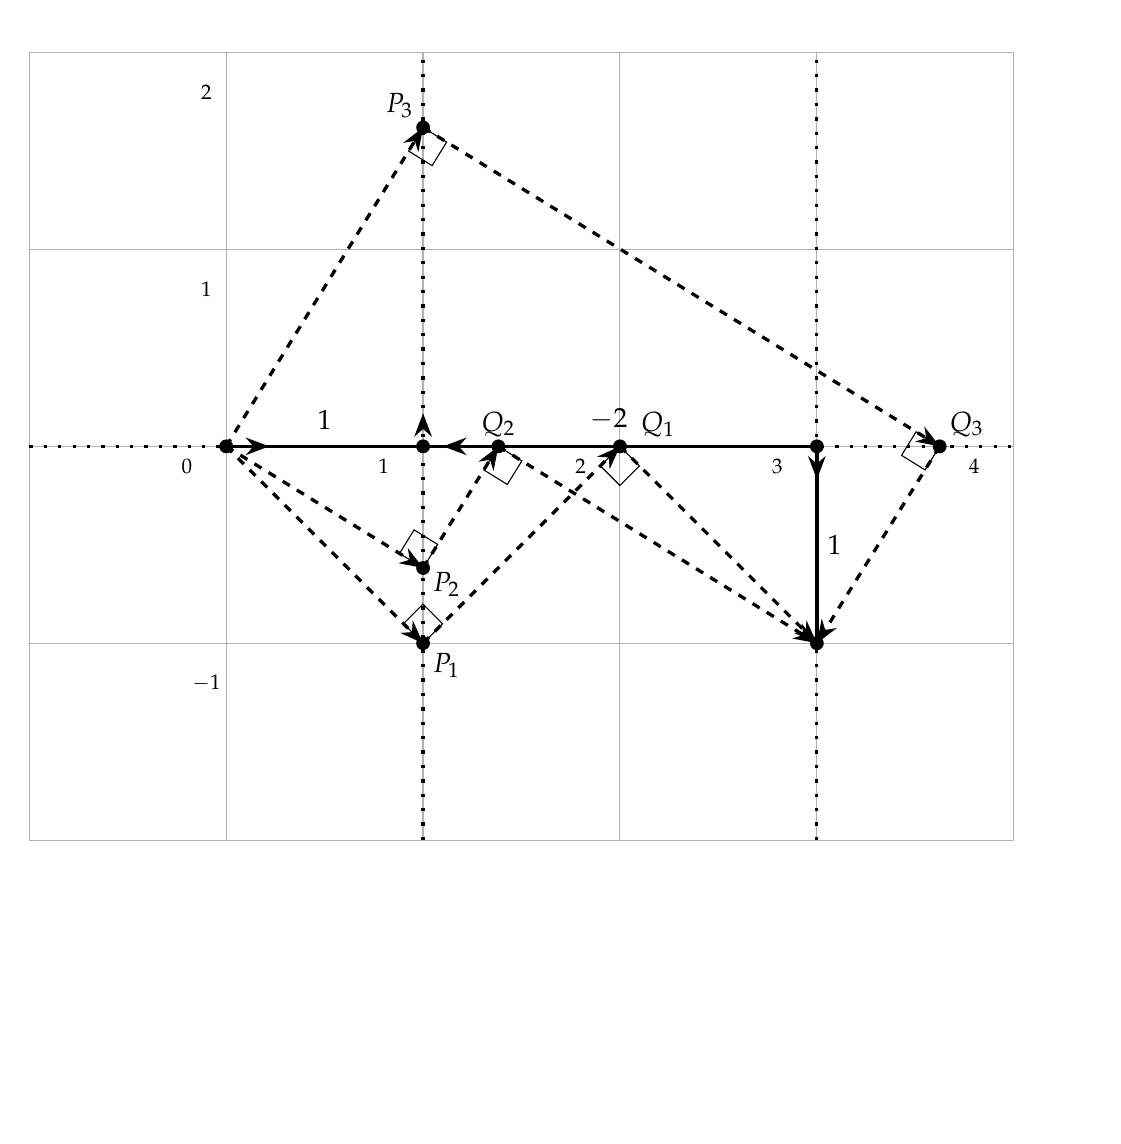
\begin{tikzpicture}[scale=2.5]
\draw[step=10mm,white!70!black,] (-1,-2) grid (4,2);
\foreach \x in {0,...,4}
  \node at (\x-.2,-.1) {\sm{\x}};
\foreach \y in {-1}
  \node at (-.1,\y-.2) {\sm{\y}};
\foreach \y in {1,2}
  \node at (-.1,\y-.2) {\sm{\y}};
\coordinate (A) at (0,0);
\coordinate (B) at (1,0);
\coordinate (C) at (3,0);
\coordinate (D) at (3,-1);
\foreach \x in {A,B,C,D}
  \fill (\x) circle(1pt); 
\draw[very thick] (A) -- node[above,yshift=2pt] {$1$} (B);
\draw[>-,very thick] ($(A)+(.1,0)$) -- ($(A)+(.15,0)$);
\draw[>-,very thick] ($(B)+(0,.05)$) -- ($(B)+(0,.1)$);
\draw[very thick,name path=bc] (B) -- 
  node[above,xshift=-4pt,yshift=2pt] {$-2$} (C);
\draw[>-,very thick] ($(B)+(.22,0)$) -- ($(B)+(.17,0)$);
\draw[very thick,name path=cd] (C) --
  node[right] {$1$}(D);
\draw[>-,very thick] ($(C)+(0,-.05)$) -- ($(C)+(0,-.1)$);
\draw[very thick,loosely dotted,name path=b] (1,-2) -- (1,2);
\draw[very thick,loosely dotted,name path=c] (-1,0) -- (4,0);
\draw[very thick,loosely dotted,name path=d] (3,-2) -- (3,2);

\coordinate (A1) at (1,-1);
\draw[very thick,dashed,-Stealth] (0,0) -- (A1);
\fill (A1) circle (1pt);
\coordinate (B1) at (2,0);
\draw[very thick,dashed,-Stealth] (A1) -- (B1);
\fill (B1) circle (1pt);
\draw[very thick,dashed,-Stealth] (B1) -- (D);

\path[name path=a2] (0,0) -- +(-31.7:4);
\path [name intersections = {of = a2 and b, by = {A2}}];
\draw[very thick,dashed,-Stealth] (0,0) -- (A2);
\fill (A2) circle (1pt);
\path[name path=b2] (A2) -- +(58.3:2.5);
\path [name intersections = {of = b2 and c, by = {B2}}];
\draw[very thick,dashed,-Stealth] (A2) -- (B2);
\fill (B2) circle (1pt);
\draw[very thick,dashed,-Stealth] (B2) -- (D);

\path[name path=a3] (0,0) -- +(58.3:2.5);
\path [name intersections = {of = a3 and b, by = {A3}}];
\draw[very thick,dashed,-Stealth] (0,0) -- (A3);
\fill (A3) circle (1pt);
\path[name path=b3] (A3) -- +(-31.7:4);
\path [name intersections = {of = b3 and c, by = {B3}}];
\draw[very thick,dashed,-Stealth] (A3) -- (B3);
\fill (B3) circle (1pt);
\path[name path=c3] (B3) -- +(-121.7:4);
\draw[very thick,dashed,-Stealth] (B3) -- (D);

\draw[rotate=58.3]   (A2) rectangle +(4pt,4pt);
\draw[rotate=-121.7] (B2) rectangle +(4pt,4pt);
\draw[rotate=-121.7]   (A3) rectangle +(4pt,4pt);
\draw[rotate=-211.7]   (B3) rectangle +(4pt,4pt);
\draw[rotate=45] (A1) rectangle +(4pt,4pt);
\draw[rotate=-135] (B1) rectangle +(4pt,4pt);

\node[below right] at (A1) {$P_1$};
\node[above right,xshift=4pt] at (B1) {$Q_1$};
\node[below right,yshift=2pt] at (A2) {$P_2$};
\node[above] at (B2) {$Q_2$};
\node[above left] at (A3) {$P_3$};
\node[above right] at (B3) {$Q_3$};
\end{tikzpicture}
\end{center}

\newpage

\section{The cube root of two}\label{s.cube}

Finally, let's check that $\sqrt[3]{2}\approx 1.26$.

In the construction of the first path, we turn twice without drawing any line segments, because the coefficients of both $x^2$ and $x$ are zero. The first segment of the second path is drawn at an angle of $-51.6^\circ$ and $(-\tan -51.6^\circ)\approx 1.26\approx \sqrt[3]{2}$.

\begin{center}
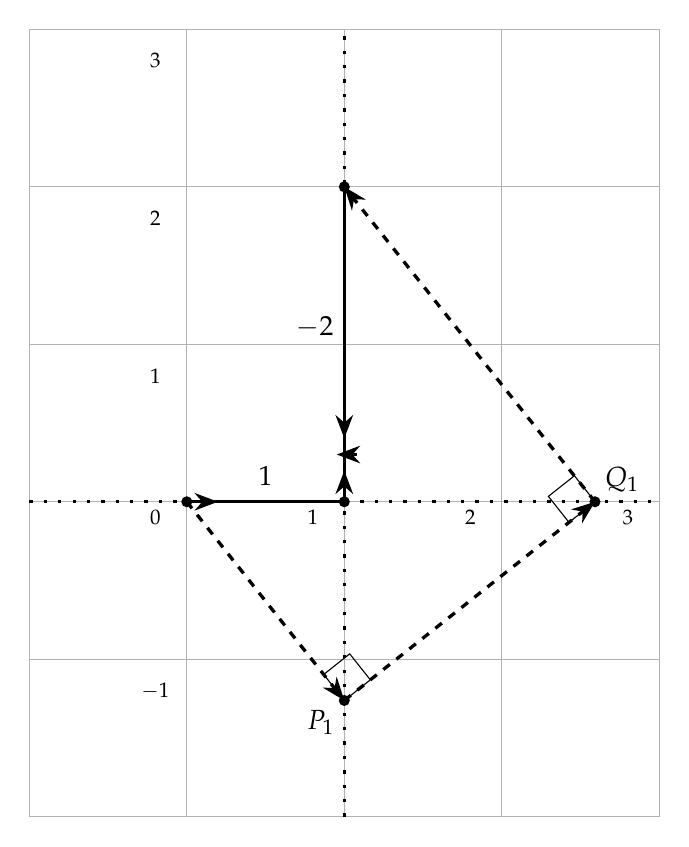
\begin{tikzpicture}[scale=2]
\draw[step=10mm,white!70!black,] (-1,-2) grid (3,3);
\foreach \x in {0,...,3}
  \node at (\x-.2,-.1) {\sm{\x}};
\foreach \y in {-1}
  \node at (-.2,\y-.2) {\sm{\y}};
\foreach \y in {1,2,3}
  \node at (-.2,\y-.2) {\sm{\y}};
\coordinate (A) at (0,0);
\coordinate (B) at (1,0);
\coordinate (C) at (1,2);
\foreach \x in {A,B,C}
  \fill (\x) circle(1pt); 
\draw[very thick] (A) -- node[above,yshift=2pt] {$1$} (B);

\draw[>-,very thick] ($(A)+(.05,0)$) -- ($(A)+(.1,0)$);
\draw[>-,very thick] ($(B)+(0,.05)$) -- ($(B)+(0,.1)$);
\draw[>-,very thick] ($(B)+(.1,.3)$) -- ($(B)+(.08,.3)$);
\draw[>-,very thick] ($(B)+(0,.55)$) -- ($(B)+(0,.5)$);

\draw[very thick] (B) -- 
  node[left,yshift=6pt] {$-2$} (C);

\draw[very thick,loosely dotted,name path=a] (-1,0) -- (3,0);
\draw[very thick,loosely dotted,name path=b] (1,-2) -- (1,3);

\path[name path=a1] (0,0) -- +(-51.6:2);
\path [name intersections = {of = a1 and b, by = {A1}}];
\draw[very thick,dashed,-Stealth] (A) -- (A1);
\fill (A1) circle (1pt);

\path[name path=b1] (A1) -- +(38.4:2.5);
\path [name intersections = {of = b1 and a, by = {B1}}];
\draw[very thick,dashed,-Stealth] (A1) -- (B1);
\fill (B1) circle (1pt);
\draw[very thick,dashed,-Stealth] (B1) -- (C);
\draw[rotate=38.4]   (A1) rectangle +(6pt,6pt);
\draw[rotate=128.4] (B1) rectangle +(6pt,6pt);

\node[below left] at (A1) {$P_1$};
\node[above right] at (B1) {$Q_1$};
\end{tikzpicture}
\end{center}

Once we have a real root of two, we can compute the two complex roots as follows. Since $\sqrt[3]{2}=\sqrt[3]{2\cdot 1}=\sqrt[3]{2}\cdot\sqrt[3]{1}$, it is sufficient to find the cube roots of one, that is, the roots of the polynomial $x^3-1$. One root is $1$ and dividing by $x-1$ gives a quadratic equation:
\[
x^3-1=(x-1)(x^2+x+1)\,.
\]
Now use the formula for finding the roots of a quadratic polynomial:
\[
r=\disfrac{-1\pm\sqrt{b^2-4ac}}{2}=\disfrac{-1\pm\sqrt{1-4}}{2}=\disfrac{-1\pm i\sqrt{3}}{2}\,.
\]
Check that:
\[
\left(\sqrt[3]{2}\cdot \disfrac{-1\pm i\sqrt{3}}{2}\right)^3=2\,.
\]


\newpage

\section{Proof of Lill's method}\label{s.proof}

We limit ourselves to monic cubic polynomials $p(x)=x^3+a_2x^2+a_1x+a_0$.\footnote{If the polynomial is not monic, divide it by $a_3$ and the resulting monic polynomial has the same roots.} In the diagram below, segments of the first path are labeled with coefficients and with $b_2,b_1,a_2-b_2,a_1-b_1$.

Since the sum of the angles of a triangle is $180^\circ$, in a right triangle if one acute angle is $\theta$, the other is $90^\circ-\theta$. Therefore, the angle above $P$ and the angle to the left of $Q$ are equal to $\theta$. The following sequence of computations follows:
\begin{form}{1.5}
\tan \theta &=& \disfrac{b_2}{1}=b_2\\
%a_2-b_2&=&a_2-\tan\theta\\
\tan \theta &=& \disfrac{b_1}{a_2-b_2}=\disfrac{b_1}{a_2-\tan\theta}\\
b_1&=&\tan\theta (a_2-\tan\theta)\\
\tan \theta &=& \disfrac{a_0}{a_1-b_1}=\disfrac{a_0}{a_1-\tan\theta(a_2-\tan\theta)}\,.
\end{form}
Simplifying the last equation gives:
\begin{form}{1.2}
(\tan\theta)^3-a_2(\tan\theta)^2+a_1(\tan\theta)-a_0=0\\
-(\tan\theta)^3+a_2(\tan\theta)^2-a_1(\tan\theta)+a_0=0\\
(-\tan\theta)^3+a_2(-\tan\theta)^2+a_1(-\tan\theta)+a_0=0\,.
\end{form}
We conclude that $-\tan\theta$ is a real root of $x^3+a_2x^2+a_1x+a_0$.


\begin{center}
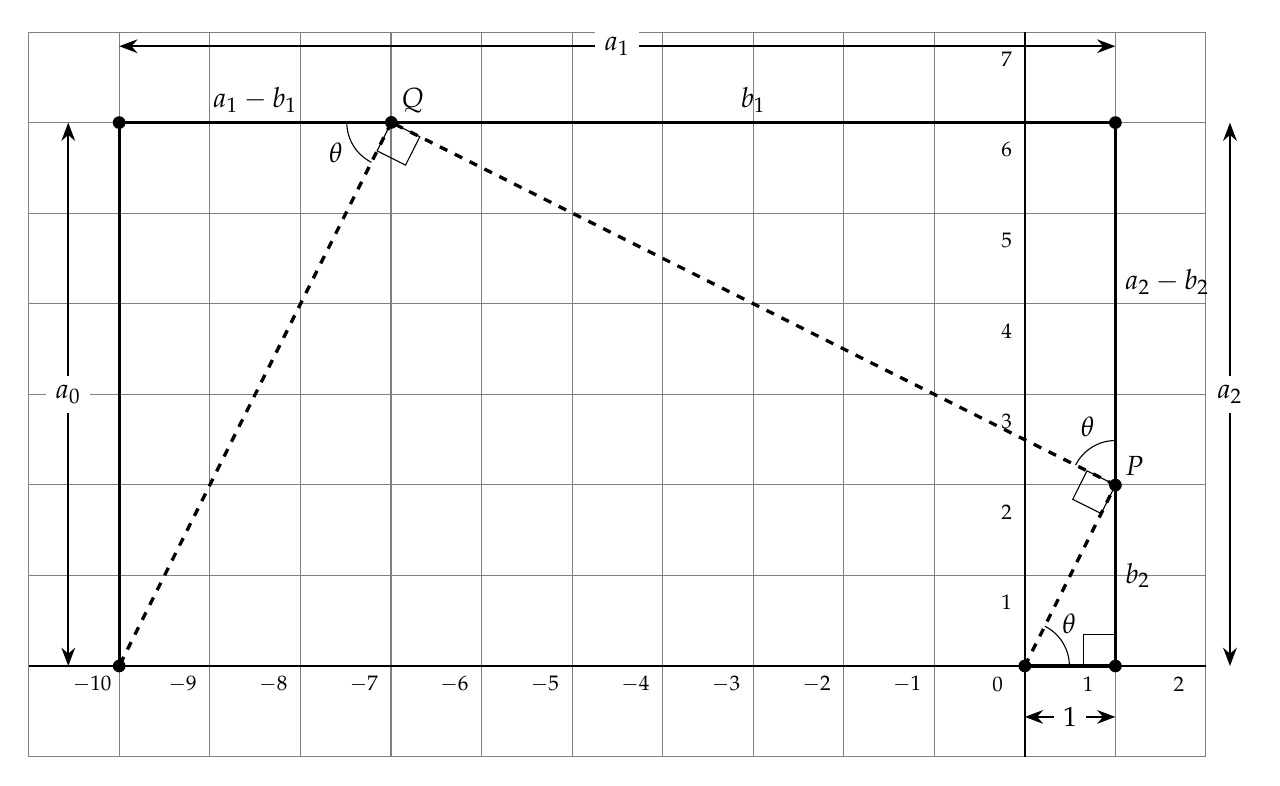
\begin{tikzpicture}[scale=1.15]
% Draw grid and axes
\draw[step=10mm,white!50!black] (-11,-1) grid (2,7);
\draw[thick] (-11,0) -- (2,0);
\draw[thick] (0,-1) -- (0,7);
\foreach \x in {-10,...,2}
  \node at (\x-.3,-.2) {\sm{\x}};
\foreach \y in {1,...,7}
  \node at (-.2,\y-.3) {\sm{\y}};
  
% Draw the points of the first path
\coordinate (A) at (0,0);
\coordinate (B) at (1,0);
\coordinate (C) at (1,6);
\coordinate (D) at (-10,6);
\coordinate (E) at (-10,0);
\foreach \x in {A,B,C,D,E}
  \fill (\x) circle(2pt);
\draw[rotate=90] (B) rectangle +(10pt,10pt);
  
% Draw A -- B and arrow
\draw[very thick] (A) --(B);
\draw[thick,<->] ($(A)+(0,-16pt)$) -- node[fill=white] {$1$} ($(B)+(0,-16pt)$);

% Draw B -- C and arrow
\draw[very thick,name path=bc] (B) -- (C);
\draw[thick,<->] ($(B)+(36pt,0)$) -- node[fill=white] {$a_2$} ($(C)+(36pt,0)$);

% Draw C -- D and arrow
\draw[very thick,name path=cd] (C) --(D);
\draw[thick,<->] ($(C)+(0,24pt)$) -- node[fill=white] {$a_1$} ($(D)+(0,24pt)$);

% Draw D -- E and arrow
\draw[very thick,name path=de] (D) -- (E);
\draw[thick,<->] ($(D)+(-16pt,0)$) -- node[fill=white] {$a_0$} ($(E)+(-16pt,0)$);

% Draw first angled segment of the second path and intersection A2 with BC
\path[name path=a2] (A) -- +(63.4:4);
\path [name intersections = {of = a2 and bc, by = {A2}}];
\fill (A2) circle(2pt) node[above right] {$P$};
\draw[very thick,dashed] (A) -- (A2);
\path (B) -- node[right] {$b_2$} (A2);
\path (A2) -- node[right,yshift=8pt] {$a_2-b_2$} (C);
\draw[rotate=153.4] (A2) rectangle +(10pt,10pt);

% Draw second segment of the second path and intersection B2 with CD
\path[name path=b2] (A2) -- +(153.4:10);
\path [name intersections = {of = b2 and cd, by = {B2}}];
\fill (B2) circle(2pt) node[above right] {$Q$};
\draw[very thick,dashed] (A2) -- (B2);
\draw[rotate=243.4] (B2) rectangle +(10pt,10pt);
\path (D) -- node[above] {$a_1-b_1$} (B2); 
\path (B2) -- node[above] {$b_1$} (C);

% Draw third segment of the second path to E
\draw[very thick,dashed] (B2)-- (E);

% Label A, A2, B2 with theta
\draw ($(A) + (14pt,0)$)
  arc [start angle=0, end angle = 63.4, radius=14pt];
\node[above right,xshift=10pt,yshift=8pt] at (A) {$\theta$};
\draw ($(A2) + (0,14pt)$)
  arc [start angle=90, end angle = 153.4, radius=14pt];
\node[above left,xshift=-4pt,yshift=14pt] at (A2) {$\theta$};
\draw ($(B2) + (-14pt,0)$)
  arc [start angle=180, end angle = 243.4, radius=14pt];
\node[below left,xshift=-14pt,yshift=-4pt] at (B2) {$\theta$};

\end{tikzpicture}
\end{center}

\newpage

\section{Lill's method and Beloch's fold}\label{s.origami}

\bibliographystyle{plain}
\bibliography{lill}

\end{document}

% !TeX root = origami-math-en.tex

%%%%%%%%%%%%%%%%%%%%%%%%%%%%%%%%%%%%%%%%%%%%%%%%%%%%%%%%%%%%%%%%
\chapter{Beloch's Fold and Beloch's Square}\label{c.beloch}

\section{The Beloch fold}\label{s.beloch-fold}

Margharita P. Beloch discovered a remarkable connection between origami and Lill's method for finding roots of polynomials. She found that one application of the operation of origami Axiom~6 (Section~\ref{s.ax6}) applied to the first path of Lill's method can obtain a real root of any cubic polynomial. The operation is often called the \emph{Beloch fold}.

Consider the polynomial $p(x)=x^3+6x^2+11x+6$ from Section~\ref{s.magic}. In the following diagram we have emphasized the second path and renamed some vertices. All we have to do to solve the equation is to perform a Beloch fold to simultaneously place the points $P',Q'$ on the line segments of lengths $a_2,a_1$, respectively. Unfortunately, if you perform the fold, the path does not solve the equation: $Q'$ is way off to the right, so the angles at $P'$ and $Q'$ are not right angles.
\begin{center}
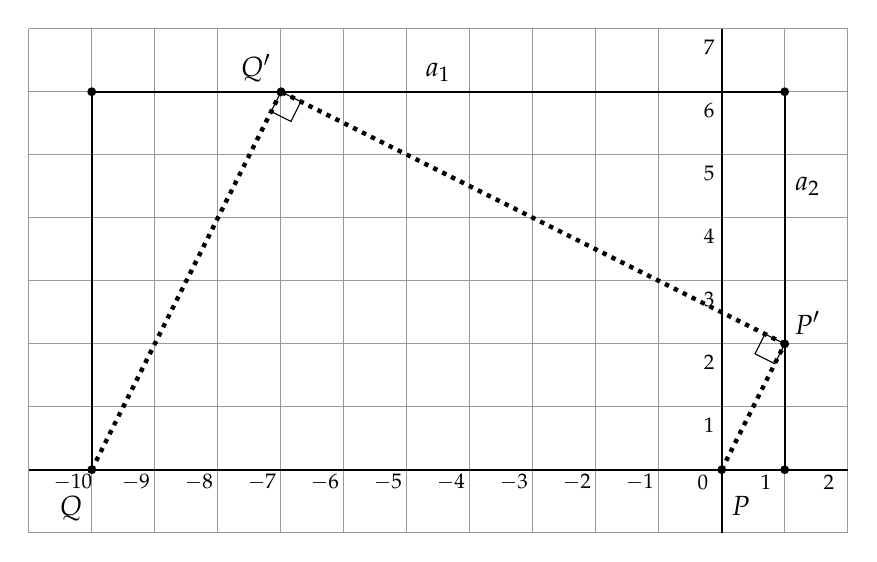
\begin{tikzpicture}[scale=.8]
% Draw help lines and axes
\draw[step=10mm,white!60!black] (-11,-1) grid (2,7);
\draw[thick] (-11,0) -- (2,0);
\draw[thick] (0,-1) -- (0,7);
\foreach \x in {-10,...,2}
  \node at (\x-.3,-.2) {\sm{\x}};
\foreach \y in {1,...,7}
  \node at (-.2,\y-.3) {\sm{\y}};
  
%Draw first path with five points
\coordinate (A) at (0,0);
\coordinate (B) at (1,0);
\coordinate (C) at (1,6);
\coordinate (D) at (-10,6);
\coordinate (E) at (-10,0);
\foreach \x in {A,B,C,D,E}
  \fill (\x) circle(2pt);
\node[below right,yshift=-6pt]  at (A) {$P$};
\node[below left,yshift=-6pt] at (E) {$Q$};

\draw[thick] (A) -- (B);
\draw[thick,name path=bc] (B) --
  node[right,near end] {$a_2$} (C);
\draw[thick,name path=cd] (C) -- 
  node[above] {$a_1$} (D);
\draw[thick,name path=de] (D) -- (E);

% Draw first segment of second path
\path[name path=a2] (A) -- +(63.4:4);
\path [name intersections = {of = a2 and bc, by = {A2}}];
\fill (A2) circle(2pt) node[above right] {$P'$};
\draw[ultra thick,dotted] (A) -- (A2);
\draw[rotate=153.4] (A2) rectangle +(10pt,10pt);

% Draw second segment of second path
\path[name path=b2] (A2) -- +(153.4:10);
\path [name intersections = {of = b2 and cd, by = {B2}}];
\fill (B2) circle(2pt) node[above left]  {$Q'$};
\draw[ultra thick,dotted] (A2) -- (B2);
\draw[rotate=243.4] (B2) rectangle +(10pt,10pt);

% Draw third segment of second path
\draw[ultra thick,dotted] (B2) -- (E);
\end{tikzpicture}
\end{center}

\newpage

Recall that a fold is the perpendicular bisector of the line segment between any point and its reflection around the fold. We want $\overline{P'Q'}$ to be a fold so that it will be perpendicular to both $\overline{QQ'}$ and $\overline{PP'}$. If $\overline{P'Q'}$ is the perpendicular bisector of $\overline{QQ'}$ and $\overline{PP'}$, then $P',Q'$, the reflections of $P,Q$, must be the same distance away from the fold as $P$ and $Q$, respectively. With some change of notation we have the following diagram.

\begin{center}
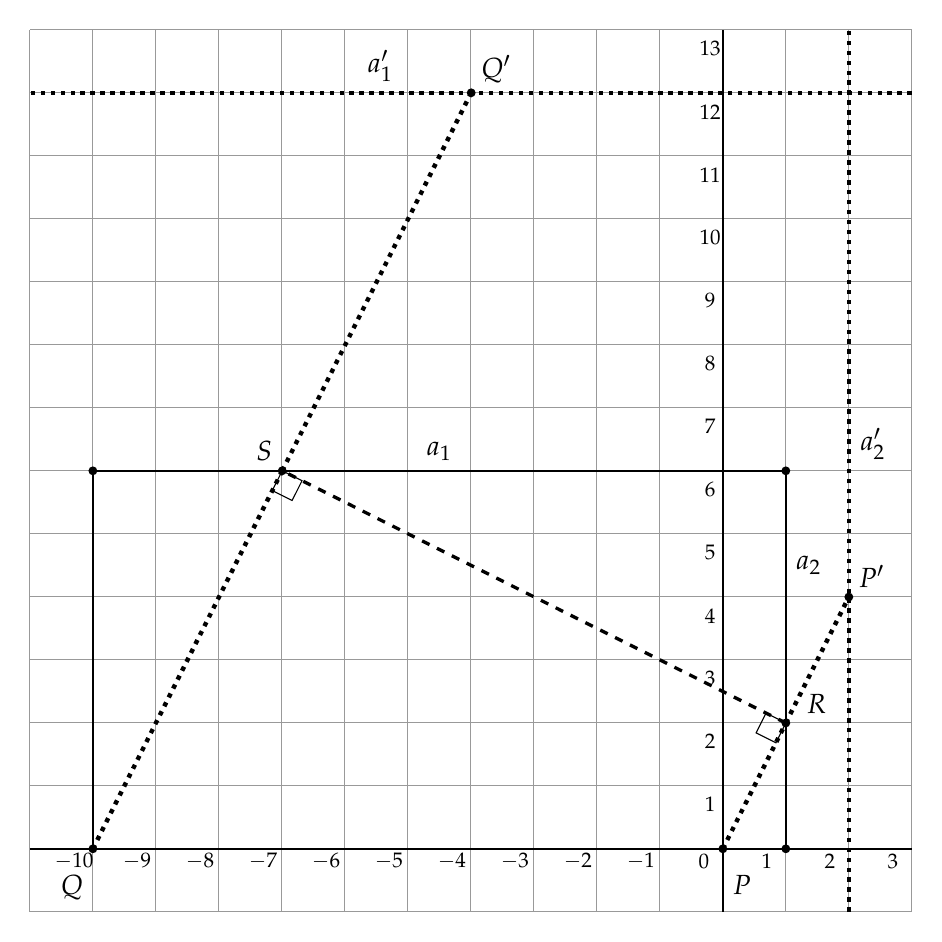
\begin{tikzpicture}[scale=.8]
% Draw help lines and axes
\draw[step=10mm,white!60!black] (-11,-1) grid (3,13);
\draw[thick] (-11,0) -- (3,0);
\draw[thick] (0,-1) -- (0,13);
\foreach \x in {-10,...,3}
  \node at (\x-.3,-.2) {\sm{\x}};
\foreach \y in {1,...,13}
  \node at (-.2,\y-.3) {\sm{\y}};
  
% Draw first path with five points
\coordinate (A) at (0,0);
\coordinate (B) at (1,0);
\coordinate (C) at (1,6);
\coordinate (D) at (-10,6);
\coordinate (E) at (-10,0);
\foreach \x in {A,B,C,D,E}
  \fill (\x) circle(2pt);
\node[below right,yshift=-6pt] at (A) {$P$};
\node[below left,yshift=-6pt] at (E) {$Q$};

\draw[thick] (A) -- (B);
\draw[thick,name path=bc] (B) -- node[right,near end] {$a_2$} (C);
\draw[thick,name path=cd] (C) -- node[above] {$a_1$} (D);
\draw[thick,name path=de] (D) -- (E);

% Draw parallel lines
\draw[ultra thick,dotted,name path=bpcp] ($(B)+(1,-1)$) --
  node[above right] {$a_2'$}
  ($(C)+(1,7)$);
\draw[ultra thick,dotted,name path=cpdp] ($(C)+(2,6)$) -- 
  node[above left,xshift=-24pt] {$a_1'$} 
  ($(D)+(-1,6)$);

% Draw first segment of second path
\path[name path=a2] (A) -- +(63.4:4);
\path [name intersections = {of = a2 and bc, by = {A2}}];
\draw[ultra thick,dotted] (A) -- (A2);
\fill (A2) circle(2pt) node[above right,xshift=4pt] {$R$};
\draw[rotate=153.4] (A2) rectangle +(10pt,10pt);

% Draw second segment of second path
\path[name path=b2] (A2) -- +(153.4:10);
\path [name intersections = {of = b2 and cd, by = {B2}}];
\fill (B2) circle(2pt) node[above left]  {$S$};
\draw[very thick,dashed] (A2) -- (B2);
\draw[rotate=243.4] (B2) rectangle +(10pt,10pt);

% Draw third segment of second path
\draw[ultra thick,dotted] (B2) -- (E);

% Locate reflections on parallel lines and draw lines
\coordinate (PP) at ($(A2)+(1,2)$);
\fill (PP) circle(2pt) node[above right] {$P'$};
\draw[ultra thick,dotted] (A2) -- (PP);

\coordinate (QP) at ($(B2)+(3,6)$);
\fill (QP) circle(2pt) node[above right] {$Q'$};
\draw[ultra thick,dotted] (B2) -- (QP);
\end{tikzpicture}
\end{center}


A line $a_2'$ is drawn so that it is parallel to $a_2$ and the same distance from $a_2$ as $a_2$ is from $P$. Similarly, line $a_1'$ is drawn so that it is parallel to $a_1$ and the same distance from $a_1$ as $a_1$ is from $Q$. Apply Axiom~6 to simultaneously place $P$ at $P'$ on $a_2'$ and to place $Q$ at $Q'$ on $a_1'$. The fold $\overline{RS}$ is the perpendicular bisector of the lines $\overline{PP'}$ and $\overline{QQ'}$; therefore, the angles at $R$ and $S$ are right angles as required.

\newpage

Let us try the Beloch fold on the polynomial $x^3-3x^2-3x+1$ from Section~\ref{s.negative}. $a_2$ is the vertical line segment of length $3$ whose equation is $x=1$, and its parallel line is $a_2'$ whose equation is $x=2$, because $P$ is at a distance of $1$ from $a_2$. $a_1$ is the horizontal line segment of length $3$ whose equation is $y=-3$, and its parallel line is $a_1'$ whose equation is $y=-2$ because $Q$ is at a distance of $1$ from $a_1$. The fold $RS$ is the perpendicular bisector of both $\overline{PP'}$ and $\overline{QQ'}$. The line $\overline{PRSQ}$ is the same as the second path in Section~\ref{s.negative}.

\begin{center}
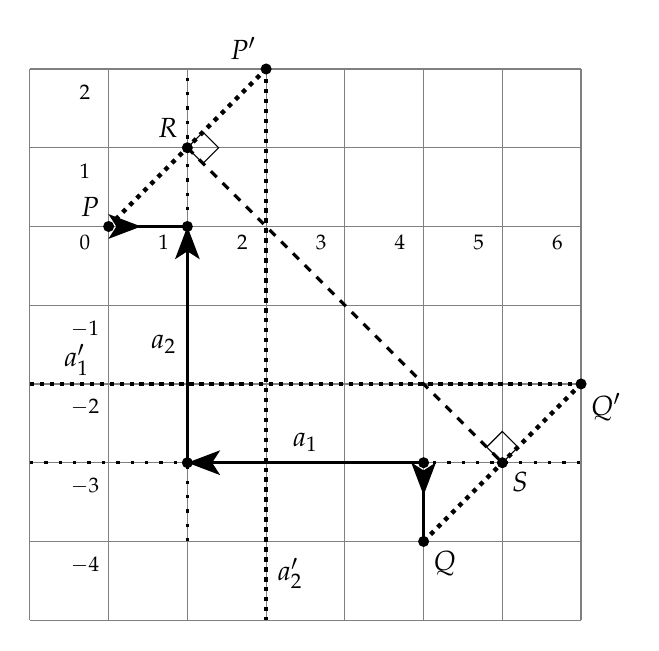
\begin{tikzpicture}[scale=1]
% Draw help lines and axes
\draw[step=10mm,white!50!black] (-1,-5) grid (6,2);
\foreach \x in {0,...,6}
  \node at (\x-.3,-.2) {\sm{\x}};
\foreach \y in {-4,...,-1}
  \node at (-.3,\y-.3) {\sm{\y}};
\foreach \y in {1,...,2}
  \node at (-.3,\y-.3) {\sm{\y}};

% Draw first path
\coordinate (A) at (0,0);
\coordinate (B) at (1,0);
\coordinate (C) at (1,-3);
\coordinate (D) at (4,-3);
\coordinate (E) at (4,-4);
\node[above left] at (A) {$P$};
\node[below right] at (E) {$Q$};
\foreach \x in {A,B,C,D,E}
  \fill (\x) circle(2pt);

\draw[very thick,{Stealth[scale=1.4,inset=2pt,reversed]}-] (A) --
  (B);
\draw[very thick,{Stealth[scale=1.4,inset=2pt]}-,name path=bc] (B) -- 
  node[left] {$a_2$} (C);
\draw[very thick,{Stealth[scale=1.4,inset=2pt]}-,name path=cd] (C) --
  node[above] {$a_1$}(D);
\draw[very thick,{Stealth[scale=1.4,inset=2pt,reversed]}-,name path=de] (D) --
 (E);

% Draw extensions of first path
\draw[very thick,loosely dotted,name path=b] (1,-4) -- (1,2);
\draw[very thick,loosely dotted,name path=c] (-1,-3) -- (6,-3);

% Draw reflected points
\coordinate (PP) at (2,2);
\coordinate (QP) at (6,-2);
\fill (PP) circle(2pt) node[above left] {$P'$};
\fill (QP) circle(2pt) node[below right] {$Q'$};

% Midpoints of bisected lines
\coordinate (R) at (1,1);
\coordinate (S) at (5,-3);
\fill (R) circle(2pt) node[above left] {$R$};
\fill (S) circle(2pt) node[below right] {$S$};

% Draw reflected lines
\draw[ultra thick,dotted] ($(B)+(1,2)$) --
  node[right,very near end,yshift=-8pt] {$a_2'$} ($(C)+(1,-2)$);
\draw[ultra thick,dotted] ($(C)+(-2,1)$) --
  node[above,very near start,xshift=-8pt,yshift=-1pt] {$a_1'$} ($(D)+(2,1)$);
\draw[ultra thick,dotted] (A) -- (PP);
\draw[ultra thick,dotted] (E) -- (QP);

% Draw fold
\draw[very thick,dashed] (R) -- (S);
\draw[rotate=-45] (R) rectangle +(8pt,8pt);
\draw[rotate=45] (S) rectangle +(8pt,8pt);
\end{tikzpicture}
\end{center}

\newpage

\section{The Beloch square}\label{s.beloch-square}

This construction in the previous section can be expressed in terms of a \emph{Beloch square}: Given two points $P,Q$ and two lines $a_2,a_1$, construct a square $\overline{ARSB}$, such that:
\begin{itemize}
\item One side is $\overline{RS}$ where $R$ lies on $a_2$ and $S$ lies on $a_1$;
\item $P$ lies on $\overline{RA}$ and $Q$ lies on $\overline{SB}$.
\end{itemize}
The following diagram extends the construction for $x^3+6x^2+11x+6$ to show the Beloch square. The length of $RS$ is $\sqrt{80}=4\sqrt{5}\approx 8.94$. We can construct the square by adding three sides of this length.
\begin{center}
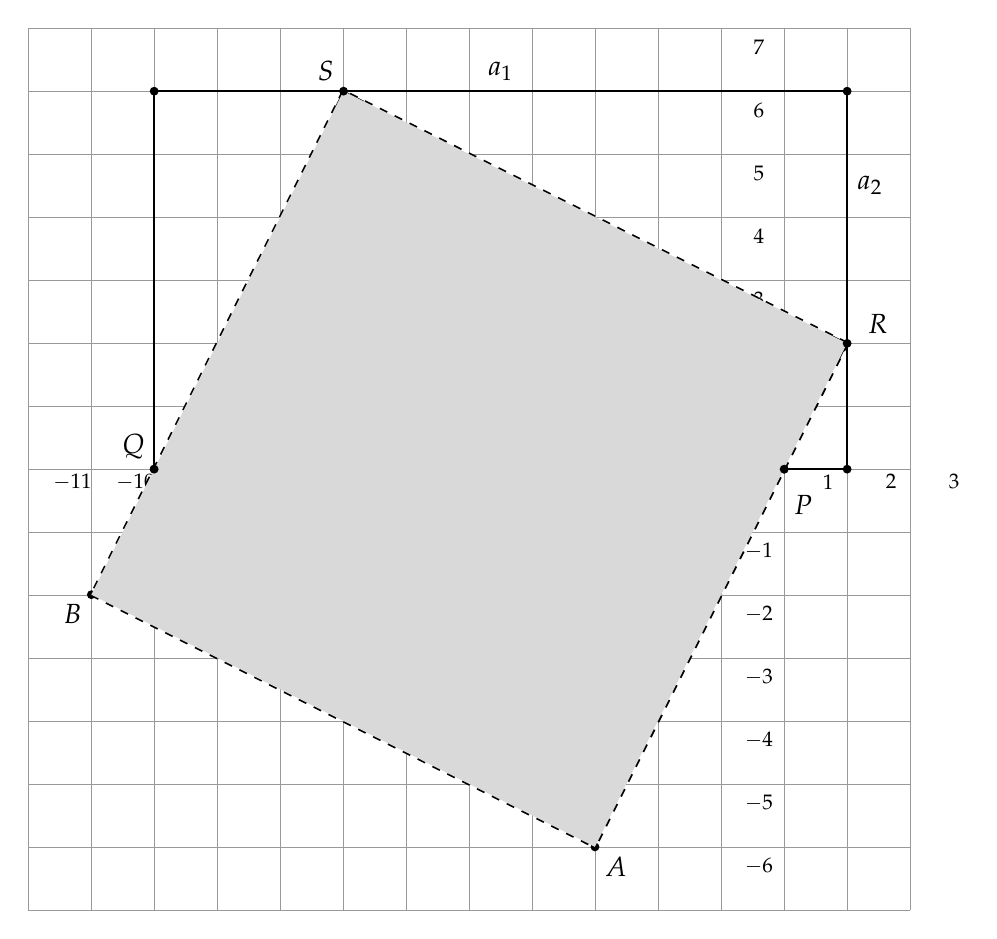
\begin{tikzpicture}[scale=.8]
% Draw help lines and axes
\draw[step=10mm,white!60!black] (-12,-7) grid (2,7);
%\draw[thick] (-12,0) -- (2,0);
%\draw[thick] (0,-7) -- (0,7);
\foreach \x in {-11,...,3}
  \node at (\x-.3,-.2) {\sm{\x}};
\foreach \y in {1,...,7}
  \node at (-.4,\y-.3) {\sm{\y}};
\foreach \y in {-6,...,-1}
  \node at (-.4,\y-.3) {\sm{\y}};

% Draw first path
\coordinate (A) at (0,0);
\coordinate (B) at (1,0);
\coordinate (C) at (1,6);
\coordinate (D) at (-10,6);
\coordinate (E) at (-10,0);
\foreach \x in {A,B,C,D,E}
  \fill (\x) circle(2pt);
\draw[thick] (A) -- (B);
\draw[thick,name path=bc] (B) -- node[right,near end] {$a_2$} (C);
\draw[thick,name path=cd] (C) -- node[above] {$a_1$} (D);
\draw[thick,name path=de] (D) -- (E);

% Find first segment of second path
\path[name path=a2] (A) -- +(63.4:4);
\path [name intersections = {of = a2 and bc, by = {A2}}];
\draw[rotate=153.4] (A2) rectangle +(10pt,10pt);

% Draw second segment of second path
\path[name path=b2] (A2) -- +(153.4:10);
\path [name intersections = {of = b2 and cd, by = {B2}}];
\draw[very thick,dashed] (A2) -- (B2);
\draw[rotate=243.4] (B2) rectangle +(10pt,10pt);

% Draw square
\draw[very thick,dashed] (B2) -- +(243.4:8.94) coordinate (AB);
\draw[very thick,dashed] (A2) -- +(243.4:8.94) coordinate (BB);
\fill (AB) circle (2pt) node[below left] {$B$};
\fill (BB) circle (2pt) node[below right] {$A$};
\draw[very thick,dashed] (AB) -- (BB);

\path[fill=white!85!black,rotate=-26.6] (AB) rectangle +(8.94,8.94);

% Draw labels of points
\fill (A2) circle(2pt) node[above right,xshift=4pt] {$R$};
\fill (B2) circle(2pt) node[above left]  {$S$};
\fill (A)  circle(2pt) node[below right,yshift=-6pt]  {$P$};
\fill (E)  circle(2pt) node[above left]  {$Q$};
\end{tikzpicture}
\end{center}


% !TeX root = origami-activities-en.tex

%%%%%%%%%%%%%%%%%%%%%%%%%%%%%%%%%%%%%%%%%%%%%%%%%%%%%%%%%%%%%%%%%%
%%%%%%%%%%%%%%%%%%%%%%%%%%%%%%%%%%%%%%%%%%%%%%%%%%%%%%%%%%%%%%%%%%
%%%%%%%%%%%%%%%%%%%%%%%%%%%%%%%%%%%%%%%%%%%%%%%%%%%%%%%%%%%%%%%%%%

\section*{Further reading}

Applications of origami \cite{lang-ted}. Mathematical theory of origami \cite{alperin,moti-origami}. History of origami \cite{history}. Paper folding \cite{lang,newton}.


\bibliographystyle{plain}
\bibliography{origami-activities-en}

% !TeX root = origami-math.tex

\appendix


\chapter{GeoGebra links}\label{a.geo}

\begin{center}
\begin{tabular}{|l|l|}
\hline
Axiom 1& \url{https://www.geogebra.org/m/fq9d5hms}\\\hline
Axiom 2& \url{https://www.geogebra.org/m/fgmfss27}\\\hline
Axiom 3& \url{https://www.geogebra.org/m/ek3mqupw}\\\hline
Axiom 4& \url{https://www.geogebra.org/m/renzzbdg}\\\hline
Axiom 5& \url{https://www.geogebra.org/m/aszn9ywu}\\\hline
Axiom 6& \url{https://www.geogebra.org/m/bxe5e5ku}\\\hline
Axiom 7& \url{https://www.geogebra.org/m/yeq5gmeg}\\\hline
Abe's trisection & \url{https://www.geogebra.org/m/dxrcvjam}\\\hline
Martin's trisection & \url{https://www.geogebra.org/m/caky7edd}\\\hline
Messer's doubling of the cube & \url{https://www.geogebra.org/m/mrcwjqh8}\\\hline
Beloch's doubling of the cube & \url{https://www.geogebra.org/m/enzmmwua}\\\hline
\end{tabular}
\end{center}
Due to a bug in Geogebra, in projects that use Axiom~6, points defined by reflection around the common tangent are not saved or are saved incorrectly.

\chapter{Derivation of trigonometric identities}\label{a.tangent}

The trigonometric identifies for tangent used in the proof of Axiom 3 can be derived from identifies for the sine and cosine:

\begin{form}{2.2}
\tan (\theta_1+\theta_2) &=& \disfrac{\sin(\theta_1+\theta_2)}{\cos(\theta_1+\theta_2)}\\
&=&\disfrac{\sin\theta_1\cos\theta_2+\cos\theta_1\sin\theta_2}{\cos\theta_1\cos\theta_2-\sin\theta_1\sin\theta_2}\\
&=&\disfrac{\sin\theta_1+\cos\theta_1\tan\theta_2}{\cos\theta_1-\sin\theta_1\tan\theta_2}\\
&=&\disfrac{\tan\theta_1+\tan\theta_2}{1-\tan\theta_1\tan\theta_2}\,.
\end{form}

We use this formula with $\theta=(\theta/2)+(\theta/2)$ to obtain a quadratic equation in $\tan(\theta/2)$:
\begin{form}{2.2}
\tan \theta=\disfrac{\tan(\theta/2)+\tan(\theta/2)}{1-\tan^2(\theta/2)}\\
\tan\theta \,(\tan(\theta/2))^2 \;+\; 2\,(\tan (\theta/2)) \;-\;\tan \theta = 0\,.
\end{form}
Its solutions are:
\[
\tan(\theta/2) = \disfrac{-1\pm\sqrt{1+\tan^2\theta}}{\tan\theta}\,.
\]

\chapter{Parabolas}\label{a.parabola}


Students are usually introduced to parabolas as the graphs of second degree equations:
\[
y=ax^2+bx+c\,.
\]
However, parabolas can be defined geometrically: given a point, the \emph{focus}, and a line, the \emph{directrix}, the locus of points equidistant from the focus and the directrix defines a parabola.


The following diagram shows the focus---the large point at $p=(0,f)$, and the directrix---the thick line whose equation is $y=-f$. The resulting parabola is shown as a dotted curve. Its vertex $p_2$ is at the origin of the axes.

%\begin{figure}[H]
\begin{center}
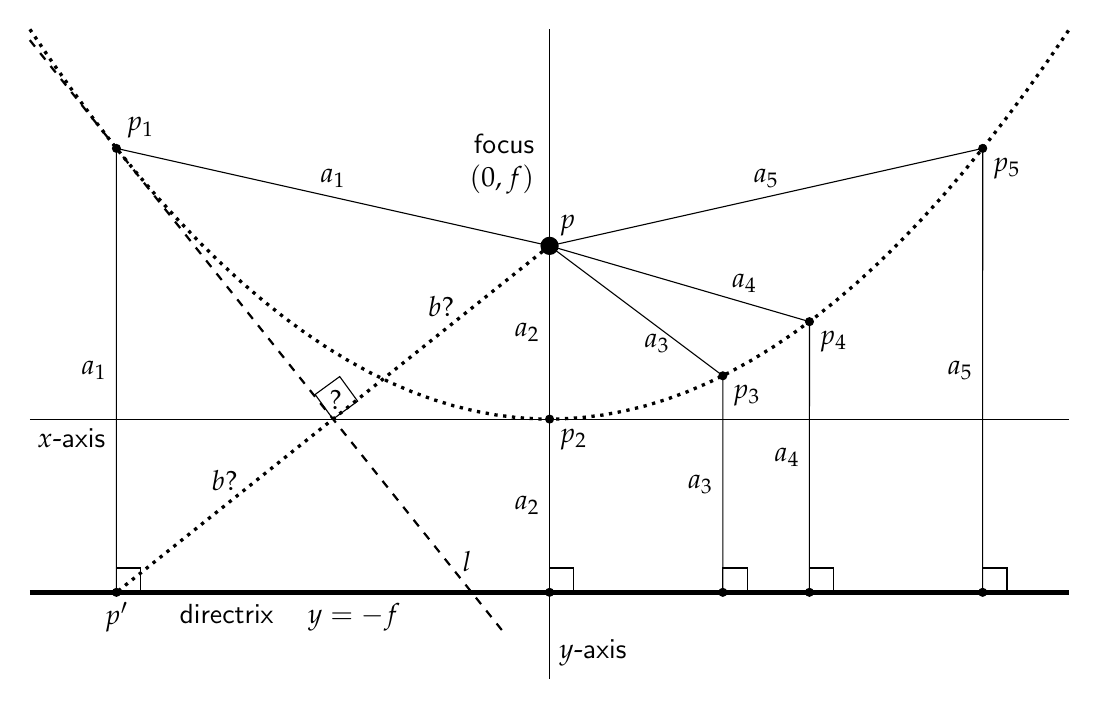
\begin{tikzpicture}[scale=1.1]
\draw (-6,0) -- node[very near start,below,xshift=-32pt] {$x$-\textsf{axis}} (6,0);
\draw (0,-3) -- node[very near start,right,yshift=-20pt] {$y$-\textsf{axis}} (0,4.5);
\draw[ultra thick] (-6,-2) -- node[near start,below] {\textsf{directrix} $\quad y=-f$} (6,-2);
\draw[domain=-6:6,samples=50,very thick,dotted] plot (\x,{\x*\x/8});
\coordinate (F) at (0,2);
\fill (F) circle (3pt) node[above left,xshift=-2pt,yshift=15pt] {$(0,f)$} node[above left,xshift=-2pt,yshift=30pt] {\textsf{focus}} node[above right] {$p$};
\fill (0,0) circle (1.5pt) node[below right] {$p_2$};
\fill (0,-2) circle (1.5pt);
\fill (2,-2) circle (1.5pt);
\fill (3,-2) circle (1.5pt);
\fill (5,-2) circle (1.5pt);
\coordinate (FP) at (-5,-2);
\fill (FP) circle (1.5pt) node[below] {$p'$};
\coordinate (F1) at (2,.5);
\fill (F1) circle (1.5pt) node[below right] {$p_3$};
\coordinate (F2) at (3,1.125);
\fill (F2) circle (1.5pt) node[below right] {$p_4$};
\coordinate (F3) at (5,3.125);
\fill (F3) circle (1.5pt) node[below right] {$p_5$};
\coordinate (F4) at (-5,3.125);
\fill (F4) circle (1.5pt) node[above right] {$p_1$};
\draw (F) -- node[left] {$a_2$} (0,0) -- node[left] {$a_2$} (0,-2);
\draw (F) -- node[near end,left] {$a_3$} (F1) -- node[left] {$a_3$} (2,-2);
\draw (F) -- node[near end,above] {$a_4$} (F2) -- node[left] {$a_4$} (3,-2);
\draw (F) -- node[above] {$a_5$} (F3) -- node[left] {$a_5$} (5,-2);
\draw (F) -- node[above] {$a_1$} (F4) -- node[left] {$a_1$} (FP);
\draw[thick,dashed] ($(F4)!-.4!(-2.5,0)$) -- node[very near end,right,xshift=2pt] {$l$} ($(F4)!1.8!(-2.5,0)$);
\draw[very thick,dotted] (F) -- (FP);
\coordinate (H) at (-2.5,0);
\node[above,xshift=1pt] at (H) {$?$};
\draw[rotate=36] (H) rectangle +(10pt,10pt);
\path (FP) -- node[above,yshift=2pt] {$b?$} (H) -- node[above,yshift=2pt] {$b?$} (F);
\draw (0,-2) rectangle +(8pt,8pt);
\draw (2,-2) rectangle +(8pt,8pt);
\draw (3,-2) rectangle +(8pt,8pt);
\draw (5,-2) rectangle +(8pt,8pt);
\draw (-5,-2) rectangle +(8pt,8pt);
\end{tikzpicture}
\end{center}
%\end{figure}

We have selected five points $p_i$, $i=1,\ldots,5$ on the parabola. Each point $p_i$ is at a distance of $a_i$ both from the focus and from the directrix.

Consider the point $p'$ that is the intersection of the perpendicular from $p_1$ to the directrix. Since $p_1$ is on the parabola $\overline{p'p_1}=\overline{p_1p}=a_1$. We claim that the tangent $l$ to the parabola at $p_1$ (dashed line) is a fold that reflects $p$ onto $p'$.

\newpage

We have to prove the $l$ is the perpendicular bisector of $\overline{pp'}$. Let us extract a simplified diagram:
\begin{center}
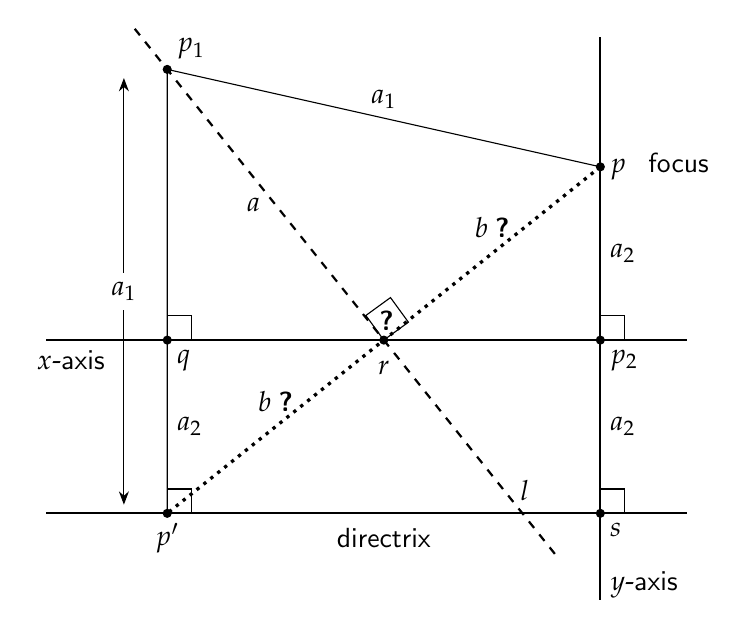
\begin{tikzpicture}[scale=1.1]
\draw[thick] (-6.4,0) -- node[very near start,below,xshift=-20pt] {$x$-\textsf{axis}} (1,0);
\draw[thick] (0,-3) -- node[very near start,right,yshift=-20pt] {$y$-\textsf{axis}} (0,3.5);
\draw[thick] (-6.4,-2) -- (1,-2);
\coordinate (F) at (0,2);
\fill (F) circle (1.5pt) node[right] {$p\;\;$ \textsf{focus}};
\fill (0,0) circle (1.5pt) node[below right] {$p_2$};
\coordinate (FP) at (-5,-2);
\fill (FP) circle (1.5pt) node[below] {$p'$};
\path (FP) -- node[below,yshift=-2pt] {\textsf{directrix}} (0,-2);
\fill (0,-2) circle (1.5pt) node[below right] {$s$};
\coordinate (F4) at (-5,3.125);
\fill (F4) circle (1.5pt) node[above right] {$p_1$};
\draw (F) -- node[right] {$a_2$} (0,0) -- node[right] {$a_2$} (0,-2);
\draw (F) -- node[above] {$a_1$} (F4) -- (FP);
\draw[<->] ($(F4)+(-.5,-.1)$) -- node[fill=white] {$a_1$}($(FP)+(-.5,.1)$);
\draw[thick,dashed] ($(F4)!-.15!(-2.5,0)$) -- node[very near end,right,xshift=2pt] {$l$} ($(F4)!1.8!(-2.5,0)$);
\draw[very thick,dotted] (F) -- (FP);
\coordinate (H) at (-2.5,0);
\node[above,xshift=1pt] at (H) {\textsf{\bfseries ?}};
\draw[rotate=36] (H) rectangle +(10pt,10pt);
\path (FP) -- node[above,yshift=2pt] {$b$ \textsf{\bfseries ?}} (H) -- node[above,yshift=2pt] {$b$ \textsf{\bfseries ?}} (F);
\draw (0,0) rectangle +(8pt,8pt);
\draw (0,-2) rectangle +(8pt,8pt);
\draw (-5,0) rectangle +(8pt,8pt);
\draw (-5,-2) rectangle +(8pt,8pt);
\fill (-5,0) circle (1.5pt) node[below right] {$q$};
\fill (-2.5,0) circle (1.5pt) node[below,yshift=-4pt] {$r$};
\path (-5,0) -- node[right] {$a_2$} (-5,-2);
\path (F4) -- node[left,xshift=-2pt] {$a$} (-2.5,0);
\end{tikzpicture}
\end{center}
\begin{itemize}
\item The directrix is parallel to the $x$-axis, the focus $p$ is on the $y$-axis and $\overline{p_1p'}$ is perpendicular to the directrix. Therefore, $\angle p'qr$ and $\angle pp_2r$ are right angles.
\item $\overline{qp'}$ and $\overline{p_2s}$ are opposite sides of a rectangle, so $\overline{qp'}=\overline{p_2s}$, which in turn is equal to $\overline{pp_2}$ since $p_2$ is on the parabola and thus equidistant from $p$ and $s$.
\item $\angle qrp'$ and $\angle p_2rp$ are equal vertical angles.
\item The right triangles $\triangle qrp'$ and $\triangle p_2rp$ have one acute angle equal and one side equal so they are congruent. Therefore, $\overline{p'r}=\overline{rp}$ and $\overline{p_1r}$ is the median of $\triangle pp_1p'$.
\item $p_1$ is on the parabola so $\overline{pp_1}=\overline{p_1p'}$. Therefore, $\triangle pp_1p'$ is an isoceles triangle.
\item In the isoceles triangle $\triangle pp_1p'$, the median $\overline{p_1r}$ is also the perpendicular bisector of $\overline{pp'}$.
\item Line $l$ contains the line segment $\overline{p_1r}$ and is the perpendicular bisector of $\overline{pp'}$.
\end{itemize}


\end{document}
